
%%%%%%%%%%%%%%%%%%%%%%%%%%%%%%%%%%%%%%%%%%%%%%%%%%%%%%%%%%%%%%%%%%%%%%%%%%%%%
%%                                                                         %%
%%                   LaTeX Vorlage für die Studenten der                   %%
%%              Dualen Hochschule Baden-Württemberg Ravensburg             %%
%%                                                                         %%
%%  Die Vorlage orientiert sich an den Gestaltungsrichtlinien der DHBW RV  %%
%%                                                                         %%
%%                                                                         %%
%% Ersteller:        Markus Schutz (WI06)                                  %%
%% letzten Änderung: 26. November 2013                                     %%
%%                                                                         %%
%%                                                                         %%
%% Wichtiger Hinweis zur Verwendung dieser Vorlage:                        %%
%%                                                                         %%
%% Damit die Vorlage verwendet und die PDF richtig und vollständig erzeugt %%
%% werden kann bedarf des manuellen Aufrufs von makeindex. Diese können    %%
%% optional auch direkt im Editor eingerichtet werden.                     %%
%% TeXnicCenter (Ausgabe -> Ausgabeprofile definieren... (Alt + F7)        %%
%%               LaTeX => PDF -> Nachbearbeitung)                          %%
%%                                                                         %%
%% (1) Stichwortverzeichnis (falls verwendet)                              %%
%% makeindex -g -s styles\stichwortverzeichnis.ist vorlage                 %%
%% (2) Abkürzungsverzeichnis                                               %%
%% makeindex vorlage.nlo -s nomencl.ist -o vorlage.nls                     %%
%% (3) Glossar (falls verwendet)                                           %%
%% makeindex -s vorlage.ist -t vorlage.glg -o vorlage.gls vorlage.glo      %%
%%                                                                         %%
%% Bei der Erzeugung der PDF Datei (Anwendung des LaTeX => PDF Ausgabe-    %%
%% profiles) werden das Abkürzungsverzeichnis, das Stichwortverzeichnis    %%
%% und das Glossar jetzt richtig erzeugt. In Verbindung mit TeXnicCenter   %%
%% kann es beim automatisierten Aufruf von makeindex zu Probleme kommen.   %%
%% Ein manueller Aufruf funktioniert dagegen immer.                        %%
%%                                                                         %%
%% Wichtiger Hinweis:                                                      %%
%%                                                                         %%
%% Keine Änderungen an den Dateien im Verzeichnis "pages" vornehmen. Für   %%
%% die Arbeit beziehen sich alle Änderungen auf diese Datei und die        %%
%% Dateien im Verzeichnis "chapter".                                       %%
%% Für die Erstellung des Literaturverzeichnises empfiehlt sich die Ver-   %%
%% wendung von JabRef (http://jabref.sourceforge.net). Die Datei ist unter %%
%% dem Namen literatur.bib im Verzeichnis "literatur" zu speichern.        %%
%% Zur sinnvollen Nutzung dieser Vorlage empfiehlt es sich, die Dokus zu   %%
%% den eingebundenen Paketen durchzulesen. Sie sind im doc-Verzeichnis der %%
%% MiKTeX-Installation zu finden.                                          %%
%%                                                                         %%
%% Enthaltene Titelblätter:                                                %%
%%   - Seminararbeit                                                       %%
%%   - Projektarbeit                                                       %%
%%   - Bachelorarbeit                                                      %%
%%                                                                         %%
%%%%%%%%%%%%%%%%%%%%%%%%%%%%%%%%%%%%%%%%%%%%%%%%%%%%%%%%%%%%%%%%%%%%%%%%%%%%%

\documentclass[a4paper,12pt]{article}                                         % Schriftgröße, Layout, Papierformat, Art des Dokumentes
\usepackage[left=3cm,right=2cm,top=2cm,bottom=2cm,includehead]{geometry}      % Einstellungen der Seitenränder
%\usepackage{ngerman}                                                          % neue Rechtschreibung
\usepackage{mathptmx}
\usepackage{csquotes}
\usepackage{acronym}
\usepackage[ngerman]{babel}                                                   % deutsche Silbentrennung
\usepackage{textgreek}
\usepackage[utf8]{inputenc}
\usepackage[table,xcdraw]{xcolor}  
\usepackage{pdflscape}   
\usepackage{rotating}                                              % Umlaute
\usepackage{booktabs} % Für \toprule, \midrule und \bottomrule
\usepackage{array}    % Für die p{}-Spalten
\usepackage{geometry} % Optional, für die Seitengröße
\usepackage{tabularx} % Automatische Breitenanpassung
\usepackage{caption}
\usepackage{subcaption}
\usepackage[hyperfootnotes=false]{hyperref}                                   % pfd-Output [Fußnoten nicht verlinken]
\usepackage[nottoc]{tocbibind}                                                % Inhaltsverzeichniserweiterung (Inhaltsverzeichnis selbst ausblenden)
\usepackage{makeidx}    % Index 
\usepackage[T1]{fontenc}
\usepackage[intoc]{nomencl}                                                   % Abkürzungsverzeichnis
\usepackage{fancyhdr}                                                         % Fancy Header
\usepackage[round]{natbib}                                                    % Zitate (Erweiterung für Literaturverzeichnis)
\usepackage{amsmath}                                                          % Zurücksetzen der Tabellen- und Abbildungsnummerierung je Sektion
\usepackage[labelfont=bf,aboveskip=1mm]{caption}                              % Bild- und Tabellenunterschrift (fett)
\usepackage{setspace}                                                         % Zeilenabstand (vor footmisc laden!)
\usepackage[bottom,multiple,hang,marginal]{footmisc}                          % Fußnoten [Ausrichtung unten, Trennung durch Seperator bei mehreren Fußnoten]
\usepackage{graphicx}                                                         % Grafiken
\usepackage{tabularx}                                                         % erweiterte Tabellen
\usepackage{longtable}                                                        % mehrseitige Tabellen
\usepackage{color}         
\usepackage{tocloft}
% Farben
\usepackage{enumitem}                                                         % Befehl setlist (Zeilenabstand für itemize Umgebung auf 1 setzen)
\usepackage{listings}                                                         % Quelltexte
\usepackage{zref}                                                             % Verweise (Anhangsverweise)
\usepackage[toc,style=altlist,translate=false]{glossaries}                    % Glossar (nach hyperref, inputenc, babel und ngerman)
\usepackage{glossaries-babel}                                                 % Glossar: Übersetzung im TOC
\usepackage{textgreek}
\usepackage{lipsum} 
\usepackage{graphicx} 
\usepackage{environ} 


\NewEnviron{SMALL}{% 
    \scalebox{0.7}{$\BODY$} 
} 


\hypersetup{
    colorlinks=true,
    linkcolor=black,
    filecolor=white,
    citecolor = black,
    urlcolor=black,
    }
\setlength{\parindent}{0em}
%%%%%%%%%%%%%%%%%%%%%%%%%%%%%%%%%%%%%%%%%%%%%%%%%%%%%%%%%%%%%%%%%%%%%%%%%%%%%
%%                                                                         %%
%% \/   \/      Bitte hier die Änderungen zur Arbeit vornehmen     \/   \/ %%
%%                                                                         %%
%%%%%%%%%%%%%%%%%%%%%%%%%%%%%%%%%%%%%%%%%%%%%%%%%%%%%%%%%%%%%%%%%%%%%%%%%%%%%

%%%%%%%%%%%%%%%%%%%%%%% Definitionen bzgl. der Arbeit %%%%%%%%%%%%%%%%%%%%%%%
\def\myType{0}           % [0=Seminararbeit|1=Projektarbeit|2=Bachelorarbeit]
\def\myTopic{Data Science- Methodik: Angewandte Geschäftsmodelle}
%\def\myMatrNr {}
\def\myKurs{WWIDS122}
\def\mySubTopic{Business Plan KARL Diagnostics}
\def\myAutor{Max Müller, Jeremy Barenkamp, Anton Geiger}
%\def\myCompany{Festo SE \& Co KG}
%\def\myCompanyAddressStreet{Ruiter Straße 82}
%\def\myCompanyAddressCity{73734 Esslingen Berkheim}
\def\myProf{Prof. Dr. Martin Zaefferer}
\def\myEndDate{30.9.2025}

%%%%%%%%%%%%%%%%%%%% Folgende Angaben für: Seminararbeit %%%%%%%%%%%%%%%%%%%%
\def\myVorlesung{Machine Learning Project}

%%%%%%%%%%%%%%%%%%%% Folgende Angaben für: Projektarbeit %%%%%%%%%%%%%%%%%%%%
\def\myProjNumber{2}         % [1|2]
\def\myPraxPhase{2}                       % [1|2|3]

%%%%%%%%%%%%%%%%%%%%%%%%%%%%%%%%%%%%%%%%%%%%%%%%%%%%%%%%%%%%%%%%%%%%%%%%%%%%%
%%                                                                         %%
%% /\   /\         Ab hier keine Änderungen mehr vornehmen         /\   /\ %%
%%                                                                         %%
%%%%%%%%%%%%%%%%%%%%%%%%%%%%%%%%%%%%%%%%%%%%%%%%%%%%%%%%%%%%%%%%%%%%%%%%%%%%%

%%%%%%%%%%%%%%%%%%%%%%%% Eigene Farbwerte definieren %%%%%%%%%%%%%%%%%%%%%%%%
\definecolor{boxgray}{gray}{0.9}         % Hintergrundfarbe für Zitatboxen
\definecolor{commentgray}{gray}{0.5}     % Grau für Kommentare in Quelltexten
\definecolor{darkgreen}{rgb}{0,.5,0}     % Grün für Strings in Quelltexten

%%%%%%%%%%%%%%%%%%%%%%%% Eigene Kommandos definieren %%%%%%%%%%%%%%%%%%%%%%%%
% Definition von \gqq{#1: text}: Text in Anführungszeichen
\newcommand{\gqq}[1]{\glqq #1\grqq}

% Definition von \footref{#1: label}
% Verweis auf bereits existierende Fußnoten mittels
\providecommand*{\footref}[1]{
	\begingroup
		\unrestored@protected@xdef\@thefnmark{\ref{#1}}
	\endgroup
\@footnotemark}

% Definition von \mypageref{#1: label}
% Kombination aus \ref{#1: label} und \pageref{#1: label}
\newcommand{\mypageref}[1]{\ref{#1} auf Seite \pageref{#1}}

% Definition von \myboxquote{#1: text}
% grau hinterlegte Quotation-Umgebung (für Zitate)
\newcommand{\myboxquote}[1]{
	\begin{quotation}{}
		\colorbox{boxgray}{\parbox{0.78\textwidth}{#1}}
	\end{quotation}
	\vspace*{1mm}
}

\makeatletter
\zref@newprop*{appsec}{}
\zref@addprop{main}{appsec}

% Definition von \applabel{#1: label}{#2: text}
% von \appsec{#1: text}{#2: label} zur Erzeugung des Labels verwendet)
\def\applabel#1#2{%
	\zref@setcurrent{appsec}{#2}%   
	\zref@wrapper@immediate{\zref@label{#1}}%
}

% Definition von \appref{#1: label}
% anstelle \ref{#1: label} zum referenzieren von Anhängen verwenden)
\def\appref#1{%
	\hyperref[#1]{\zref@extract{#1}{appsec}}%
}
\makeatother

% Definition von \appsection{#1: text}{#2: label}
% Ersetzt \section{#1: text} und \label{#2: label} für Anhänge)
\newcommand{\theappsection}[1]{Anhang \Alph{section}:~\protect #1}
\newcommand{\appsection}[2]{
	\addtocounter{section}{1}
	\phantomsection
	\addcontentsline{toc}{section}{\theappsection{#1}}
	\markboth{\theappsection{#1}}{}

	\section*{\theappsection{#1}}
	\applabel{#2}{Anhang \Alph{section}}
	\label{#2}
}

%%%%%%%%%%%%% Index, Abkürzungsverzeichnis und Glossar erstellen %%%%%%%%%%%%
\makeindex
\makenomenclature
\makeglossaries

% Festlegung der Art der Zitierung (Havardmethode: Abkuerzung Autor + Jahr) %
\bibliographystyle{mydinat}

%%%%%%%%%%%%%%%%%%%%%%%%%%%%%%% PDF-Optionen %%%%%%%%%%%%%%%%%%%%%%%%%%%%%%%%
\hypersetup{
	bookmarksopen=false,
	bookmarksnumbered=true,
	bookmarksopenlevel=0,
	pdftitle=\myTopic,
	pdfsubject=\myTopic,
	pdfauthor=\myAutor,
	pdfstartview=Fit,
	pdfpagelayout=SinglePage
}

%%%%%%%%%%%%%%%%%%%%%%%%%%%% Kopf- und Fußzeile %%%%%%%%%%%%%%%%%%%%%%%%%%%%%
\pagestyle{fancy}
\fancyhf{}
\fancyhead[R]{\thepage}                         % Kopfzeile rechts bzw. außen
\renewcommand{\headrulewidth}{0.5pt}            % Kopfzeile rechts bzw. außen

%%%%%%%%%%%%%%%%%%%%%%%%% Layout und Beschriftungen %%%%%%%%%%%%%%%%%%%%%%%%%
\onehalfspacing  % Zeilenabstand: 1.5 (Standard: 1.2)

\setlist{noitemsep}            % Zeilenabstand für items auf 1 setzen

\addto\captionsngerman{        % Tabllen- und Abbildungsunterschriften ändern
  \renewcommand{\figurename}{Abb.}
  \renewcommand{\tablename}{Tab.}
}
\numberwithin{table}{section}                               % Tabellennummerierung je Sektion zurücksetzen
\numberwithin{figure}{section}                              % Abbildungsnummerierung je Sektion zurücksetzen
\renewcommand{\thetable}{\arabic{section}.\arabic{table}}   % Tabellennummerierung mit Section
\renewcommand{\thefigure}{\arabic{section}.\arabic{figure}} % Abbildungsnummerierung mit Section
\renewcommand{\thefootnote}{\arabic{footnote}}              % Sektionsbezeichnung von Fußnoten entfernen

\renewcommand{\multfootsep}{, }                             % Mehrere Fußnoten durch ", " trennen

%%%%%%%%%%%%%%%%%%%%%%%%%%%%%%% Listingstyle %%%%%%%%%%%%%%%%%%%%%%%%%%%%%%%%
\lstset{
	basicstyle=\ttfamily\scriptsize,
	commentstyle=\color{commentgray}\textit,
	showstringspaces=false,
	stringstyle=\color{darkgreen},
	keywordstyle=\color{blue},
	numbers=left,
	numberstyle=\tiny,
	stepnumber=1,
	numbersep=15pt,
	tabsize=2,
	fontadjust=true,
	frame=single,
	backgroundcolor=\color{boxgray},
	captionpos=b,
	linewidth=0.94\linewidth,
	xleftmargin=0.1\linewidth,
	breaklines=true,
	aboveskip=16pt
}
        
%%%%%%%%%%%%%%%%%%%%%%%%%%%%%%%%%%%%%%%%%%%%%%%%%%%%%%%%%%%%%%%%%%%%%%%%%%%%%
%%                                                                         %%
%% \/   \/      Bitte hier die Änderungen zur Arbeit vornehmen     \/   \/ %%
%%                                                                         %%
%%%%%%%%%%%%%%%%%%%%%%%%%%%%%%%%%%%%%%%%%%%%%%%%%%%%%%%%%%%%%%%%%%%%%%%%%%%%%

%Seiten und Kapitel einbinden
\begin{document}{}
    %\begin{spacing}{1.5}
    
	\pagenumbering{Roman}
	% Das Titelblatt wird automatisch ausgewählt. Keine Änderung hier
	\ifcase\myType
		\begin{titlepage}
	\begin{center}
		\vspace*{2cm}
		\LARGE\bf\myTopic\\
		%\Large\rm\mySubTopic\\
		\vspace*{3cm}
		\bf
		\myVorlesung\\
		\normalsize\rm
		\vspace*{1cm}
%		für die\\
%		Prüfung zum Bachelor of Science\\
		\vspace*{1cm}
		an der Fakultät für Wirtschaft\\
		im Studiengang Wirtschaftsinformatik\\
		\vspace*{1cm}
		an der\\
		DHBW Ravensburg
		\vfill
	\end{center}
	\begin{tabular}{ll}
		Verfasser:&\myAutor\\
		%Ausbildungsbetrieb:&\myCompany\\
		%Anschrift:&\myCompanyAddressStreet\\
		%&\myCompanyAddressCity\\
		Dozent:&\myProf\\
		Abgabedatum:&\myEndDate\\
	\end{tabular}
\end{titlepage}
\newpage
\setcounter{page}{2}

	\or
		\include{pages/10_titel_projekt}
	\or
		\include{pages/10_titel_bachelor}
	\else
	\fi
	
	\pagestyle{fancy}

	\include{pages/12_inhaltsverzeichnis}
	\renewcommand{\nomname}{Abkürzungsverzeichnis}
\setlength{\nomlabelwidth}{.25\hsize}
\renewcommand{\nomlabel}[1]{#1 \dotfill}
\setlength{\nomitemsep}{-\parsep}
\printnomenclature
\section*{ \nomname {} }
\addcontentsline{toc}{section}{Abkürzungsverzeichnis}
\nomlabel{kurz} {lang} \\
\newpage

	%\renewcommand{\glossaryname}{Glossar}
\printglossaries
\section*{Glossar}
\addcontentsline{toc}{section}{Glossar}
\textbf{Eintrag 1} \\
langer Text
\\

	\include{pages/15_abbildungsverzeichnis}
	%\include{pages/16_tabellenverzeichnis}
    %\section*{Formeln}
\newcommand{\listequationsname}{}
\newlistof{myequations}{edu}{\listequationsname}
\newcommand{\myequations}[1]{%
\addcontentsline{edu}{myequations}{\protect\numberline{\theequation}#1}\par}
\listofmyequations
\newpage
	%\include{pages/17_listingsverzeichnis}
	% Kapitel
	\pagestyle{fancy}
	\fancyhead[L]{\nouppercase{\leftmark}}                               % Kopfzeile links bzw. innen
	\pagenumbering{arabic}
	\include{chapter/20_kapitel}
    \section{Executive Summary}
Stellen Sie sich eine voll belegte Werkstatt am Montagmorgen vor: Der Fehlerspeicher meldet „Dieselpartikelfilter: Differenzdruck zu hoch“, Hebebühnen sind knapp, der Kunde wartet. Was fehlt, ist nicht ein weiterer Code, sondern die wahre Ursache. Genau hier setzt \ac{KARL} Diagnostics an. Eine \ac{E2E}-Diagnoselösung aus robuster \ac{OBD}-II/\ac{CAN} Hardware (Kabel oder Funkadapter) und \ac{KI}-gestützter Cloud-Software. KARL fusioniert Fehlercodes, Live-Sensordaten, Herstellerdokumentation, Wissen aus Communities und externe Messgeräte zu präzisen, erklärbaren Reparaturempfehlungen inklusive priorisierter Hypothesen, Prüfschritte und Wahrscheinlichkeiten. Hinter einem „vollen“ Partikelfilter erkennt \ac{KARL} so etwa das defekte Thermostat als wahrscheinlichste Ursache, sichtbar in Temperatur- und Regenerationsmustern, auch ohne spezifischen Code.
\newline\newline
Für freie und markengebundene Werkstätten, Serviceketten, mobile Mechaniker, Flottenbetreiber und Prüfgesellschaften adressiert \ac{KARL} das Kernproblem steigender Komplexität bei Zeit- und Margendruck. Die Nutzen sind höhere \ac{FTFR}, weniger Teiletausch auf Verdacht, kürzere Standzeiten und produktive Unterstützung auch weniger erfahrener Mitarbeitender. Technisch setzt KARL auf eine hybride KI-Architektur aus regelbasierten Verfahren, neuronalen Netzen (z. B. LSTMs, Transformer) und einem Wissensgraphen. Jede Diagnose ist erklärbar; kontinuierliches Lernen aus realen, anonymisierten Werkstattfällen sowie Federated Learning verbessern die Performance fortlaufend, ohne Datenschutz zu gefährden. Im Wettbewerbsumfeld zwischen teuren, komplexen Premium-Testern (z. B. Bosch, Hella Gutmann), Nischenlösungen und \ac{OEM}-Tools positioniert sich KARL als herstellerunabhängige, kosteneffiziente und anwenderfreundliche Lösung mit \ac{KI}-gestützter Priorisierung, durchgängigen Prüfpfaden, \ac{OTA}-Updates und Integrationen in bestehende IT-Systeme.
\newline\newline
Der Markt wird getrieben von Elektrifizierung, softwaredefinierten Fahrzeugen und verschärften Vorgaben, somit steigt die Nachfrage nach \ac{SaaS}-Diagnose. \ac{KARL}s Go-to-Market startet mit Pilotierungen in DACH, Referenzkunden und Content-Marketing, gefolgt von schrittweiser Expansion in Europa. Vertrieblich kombinieren wir direkten \ac{B2B}-Verkauf mit Partnernetzwerken und technischen Kooperationen; integrationsseitig setzen wir auf Plug-and-Play in bestehenden Werkstattprozessen. Das Geschäftsmodell ist hybrid: einmalige Hardwareerlöse plus skalierbare Software-Abonnements pro Arbeitsplatz, ergänzt um Schulungen und Support. Kurzfristig investieren wir in Produktreife, Datenqualität, Zertifizierungen und Markteintritt; mittelfristig tragen Lizenzerlöse den größten Umsatzanteil bei bewusst margenträchtiger, aber nicht dominanter Hardware. Die Profitabilität ist nach ca. 2,5 Jahren geplant; zur Überbrückung negativer Cashflows sind Kredite von insgesamt rund 450.000 € vorgesehen.
\newline\newline
Hardware- und Software-\ac{MVP} bilden den Realisierungsplan, angfangen bei Auslieferung in kleinen Stückzahlen an Pilotkunden, schnelles Iterieren von Design, Funktionen und Produktionsprozessen, paralleler Aufbau der Fertigung und Akquise erster Kunden. Nach rund zwölf Monaten folgt der Markteintritt in Deutschland mit Fokus auf kleinere Werkstätten; anschließend breiteres Marketing, europäische Skalierung und perspektivisch eine selektive Öffnung Richtung \ac{B2C}. Chancen liegen in Netzwerkeffekten, Übertragbarkeit in angrenzende Domänen und dem wachsenden Bedarf an Diagnose-Know-how durch neue Antriebstechnologien. Risiken (Datenqualität, Zurückhaltung beim Wissensaustausch, rechtliche Fragen zur Datennutzung, \ac{OEM}-Wettbewerb, Investitionsbedarf) begegnen wir mit zusätzlichen Datenquellen, gezielten Roll-outs, Anreizsystemen, technischer Differenzierung und einer stringenten Partnerwahl. Operativ sichern agile Entwicklung, Qualitätsmanagement, Partnerintegration und internationale Skalierbarkeit die Umsetzung. Ein interdisziplinäres Kernteam aus Entwicklung, Data, Vertrieb und Einkauf gewährleistet schnelle Produktreife, Kundennähe und Lieferfähigkeit – flankiert von geplantem Teamausbau, Schulungen, Compliance-Prozessen und einer lernorientierten Kultur.

\section{Produkt \& Dienstleistung}
\label{sec:produkt}

\subsection{Problem \& Nutzenversprechen}
Moderne Fahrzeuge bringen eine hohe Systemkomplexität mit sich. Beispiele hierf"ur sind vernetzte Steuergeräte, eine Vielzahl an Sensoren sowie Hersteller- und modellabhängige Varianten. In der Werkstattpraxis führt dies zu Zeit- und Margendruck. Häufig werden Teile auf Verdacht getauscht, weil Fehlerspeicher nur Symptome melden, jedoch keine belastbaren Ursachen liefern. Die Folge sind niedrige Ersttrefferquoten, unnötige Fehlläufe und verlängerte Standzeiten. Gefordert ist eine Diagnose, die aus Symptomen verlässlich auf Ursachen schließt, Hypothesen transparent priorisiert und konkrete, effiziente Prüfschritte vorschlägt. Das Ergebnis sind höhere Ersttrefferquoten, kürzere Standzeiten und weniger Teiletausch auf Verdacht.

\emph{KARL Diagnostics}, das Künstliche-Auto-Reparatur-Lernsystem (KARL), verwandelt Fehlermeldungen und Livedaten in präzise Reparaturempfehlungen. Dazu kombiniert KARL robuste OBD/CAN-Diagnosehardware mit einer Cloud-Software, die Fehlercodes, Sensordatenströme, Expertenwissen und Foreninformationen zusammenführt. Das System liefert ursachenorientierte KI-Ergebnisse: priorisierte Hypothesen mit Wahrscheinlichkeiten, nachvollziehbare Prüfschritte und erklärende Begründungen, \emph{warum} ein Fehler auftritt, nicht nur \emph{dass} er auftritt. Jede bestätigte Reparatur fließt anonymisiert in die Modelle für alle Nutzer. 

Gegenüber klassischen Testern bietet KARL (i) ursachenorientierte \ac{KI} statt Code-Lesen, (ii) einen lernenden Algorithmus aus realen, anonymisierten Fällen und (iii) nahtlose Einbindung in bestehende Werkstattprozesse für \enquote{Plug-and-Play} in der Praxis. Die Hardware wird einmalig angeschafft; die Software wird pro Arbeitsplatz lizenziert. So bleiben die Einstiegshürden gering, der Nutzen skalierbar – und je mehr Datenpunkte einfließen, desto besser wird KARL.

\subsection{Produktübersicht: Hardware + Cloud-Software}
\ac{KARL} Diagnostics besteht aus mehreren eng verzahnten Bausteinen, die eine durchgängige Fehlerdiagnose vom Fahrzeug bis zur Cloud ermöglichen. Zum einen umfasst das System eine werkstatttaugliche OBD/CAN-Hardware für die Fahrzeuganbindung, zusätzliche Diagnosegeräte (Oszilloskop, Labornetzteil, Innenwiderstandsmesser, Multimeter) sowie eine leistungsfähige Cloud-Software. Diese Software verarbeitet eingehende Fehlercodes und Livedaten, leitet mittels künstlicher Intelligenz Ursachenhypothesen ab und ergänzt diese um strukturierte Prüfschritte mit zugehörigen Wahrscheinlichkeiten. Ziel ist ein \enquote{Plug-and-Play}-Einsatz in der Werkstatt bei maximaler Transparenz und Nachvollziehbarkeit der vorgeschlagenen Maßnahmen.

Die Fahrzeug-Schnittstelle ist robust, steckfertig und für den harten Dauerbetrieb in der Werkstatt konzipiert. Sie verfügt über ein stoßfestes Gehäuse, Öl- und Staubresistenz, eine kompakte Bauform sowie Status-LEDs für Verbindung und Logging. Zur Sicherstellung der Datenübertragung kommt ein redundantes System zum Einsatz, bestehend aus einer kabelgebundenen Schnittstelle und einer drahtlosen Anbindung via Bluetooth bzw. WLAN.
\begin{figure}[h!]
    \centering
    \begin{subfigure}[t]{0.45\linewidth}
        \centering
        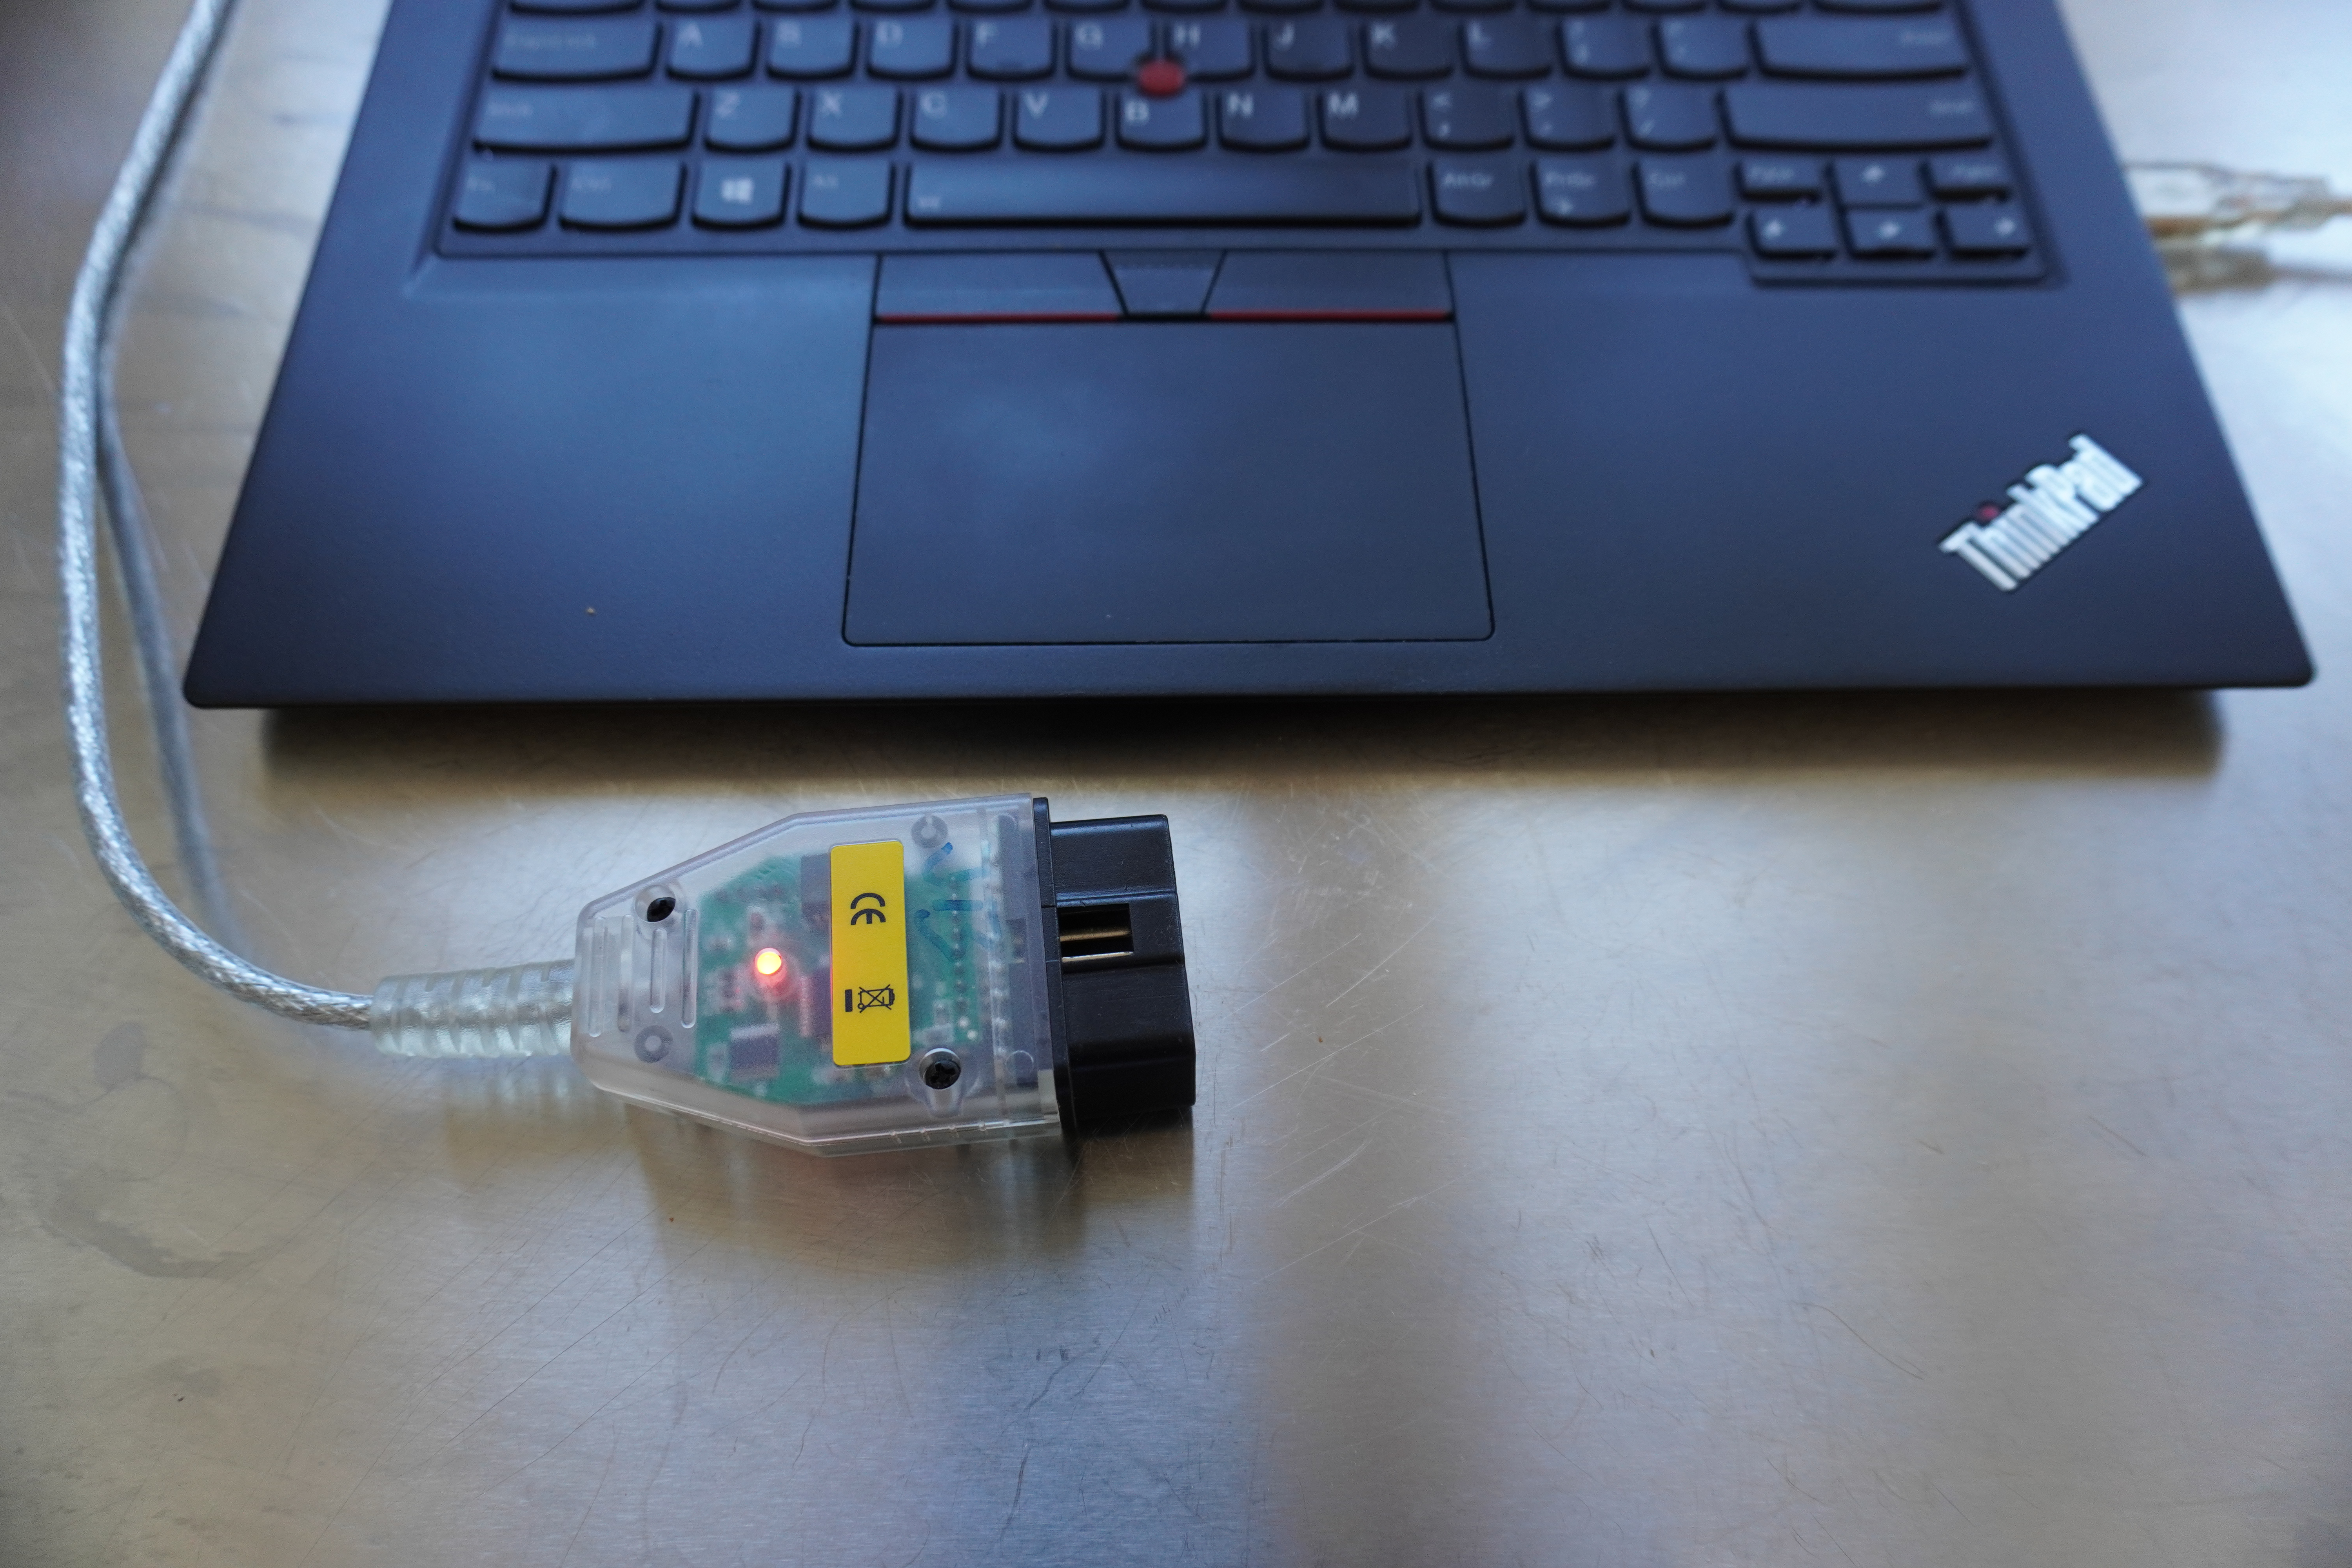
\includegraphics[width=\linewidth]{images/Hardware/obd_cable.JPG}
        \caption{OBD Kabel}
        \label{fig:obd_cable}
    \end{subfigure}
    \hfill
    \begin{subfigure}[t]{0.45\linewidth}
        \centering
        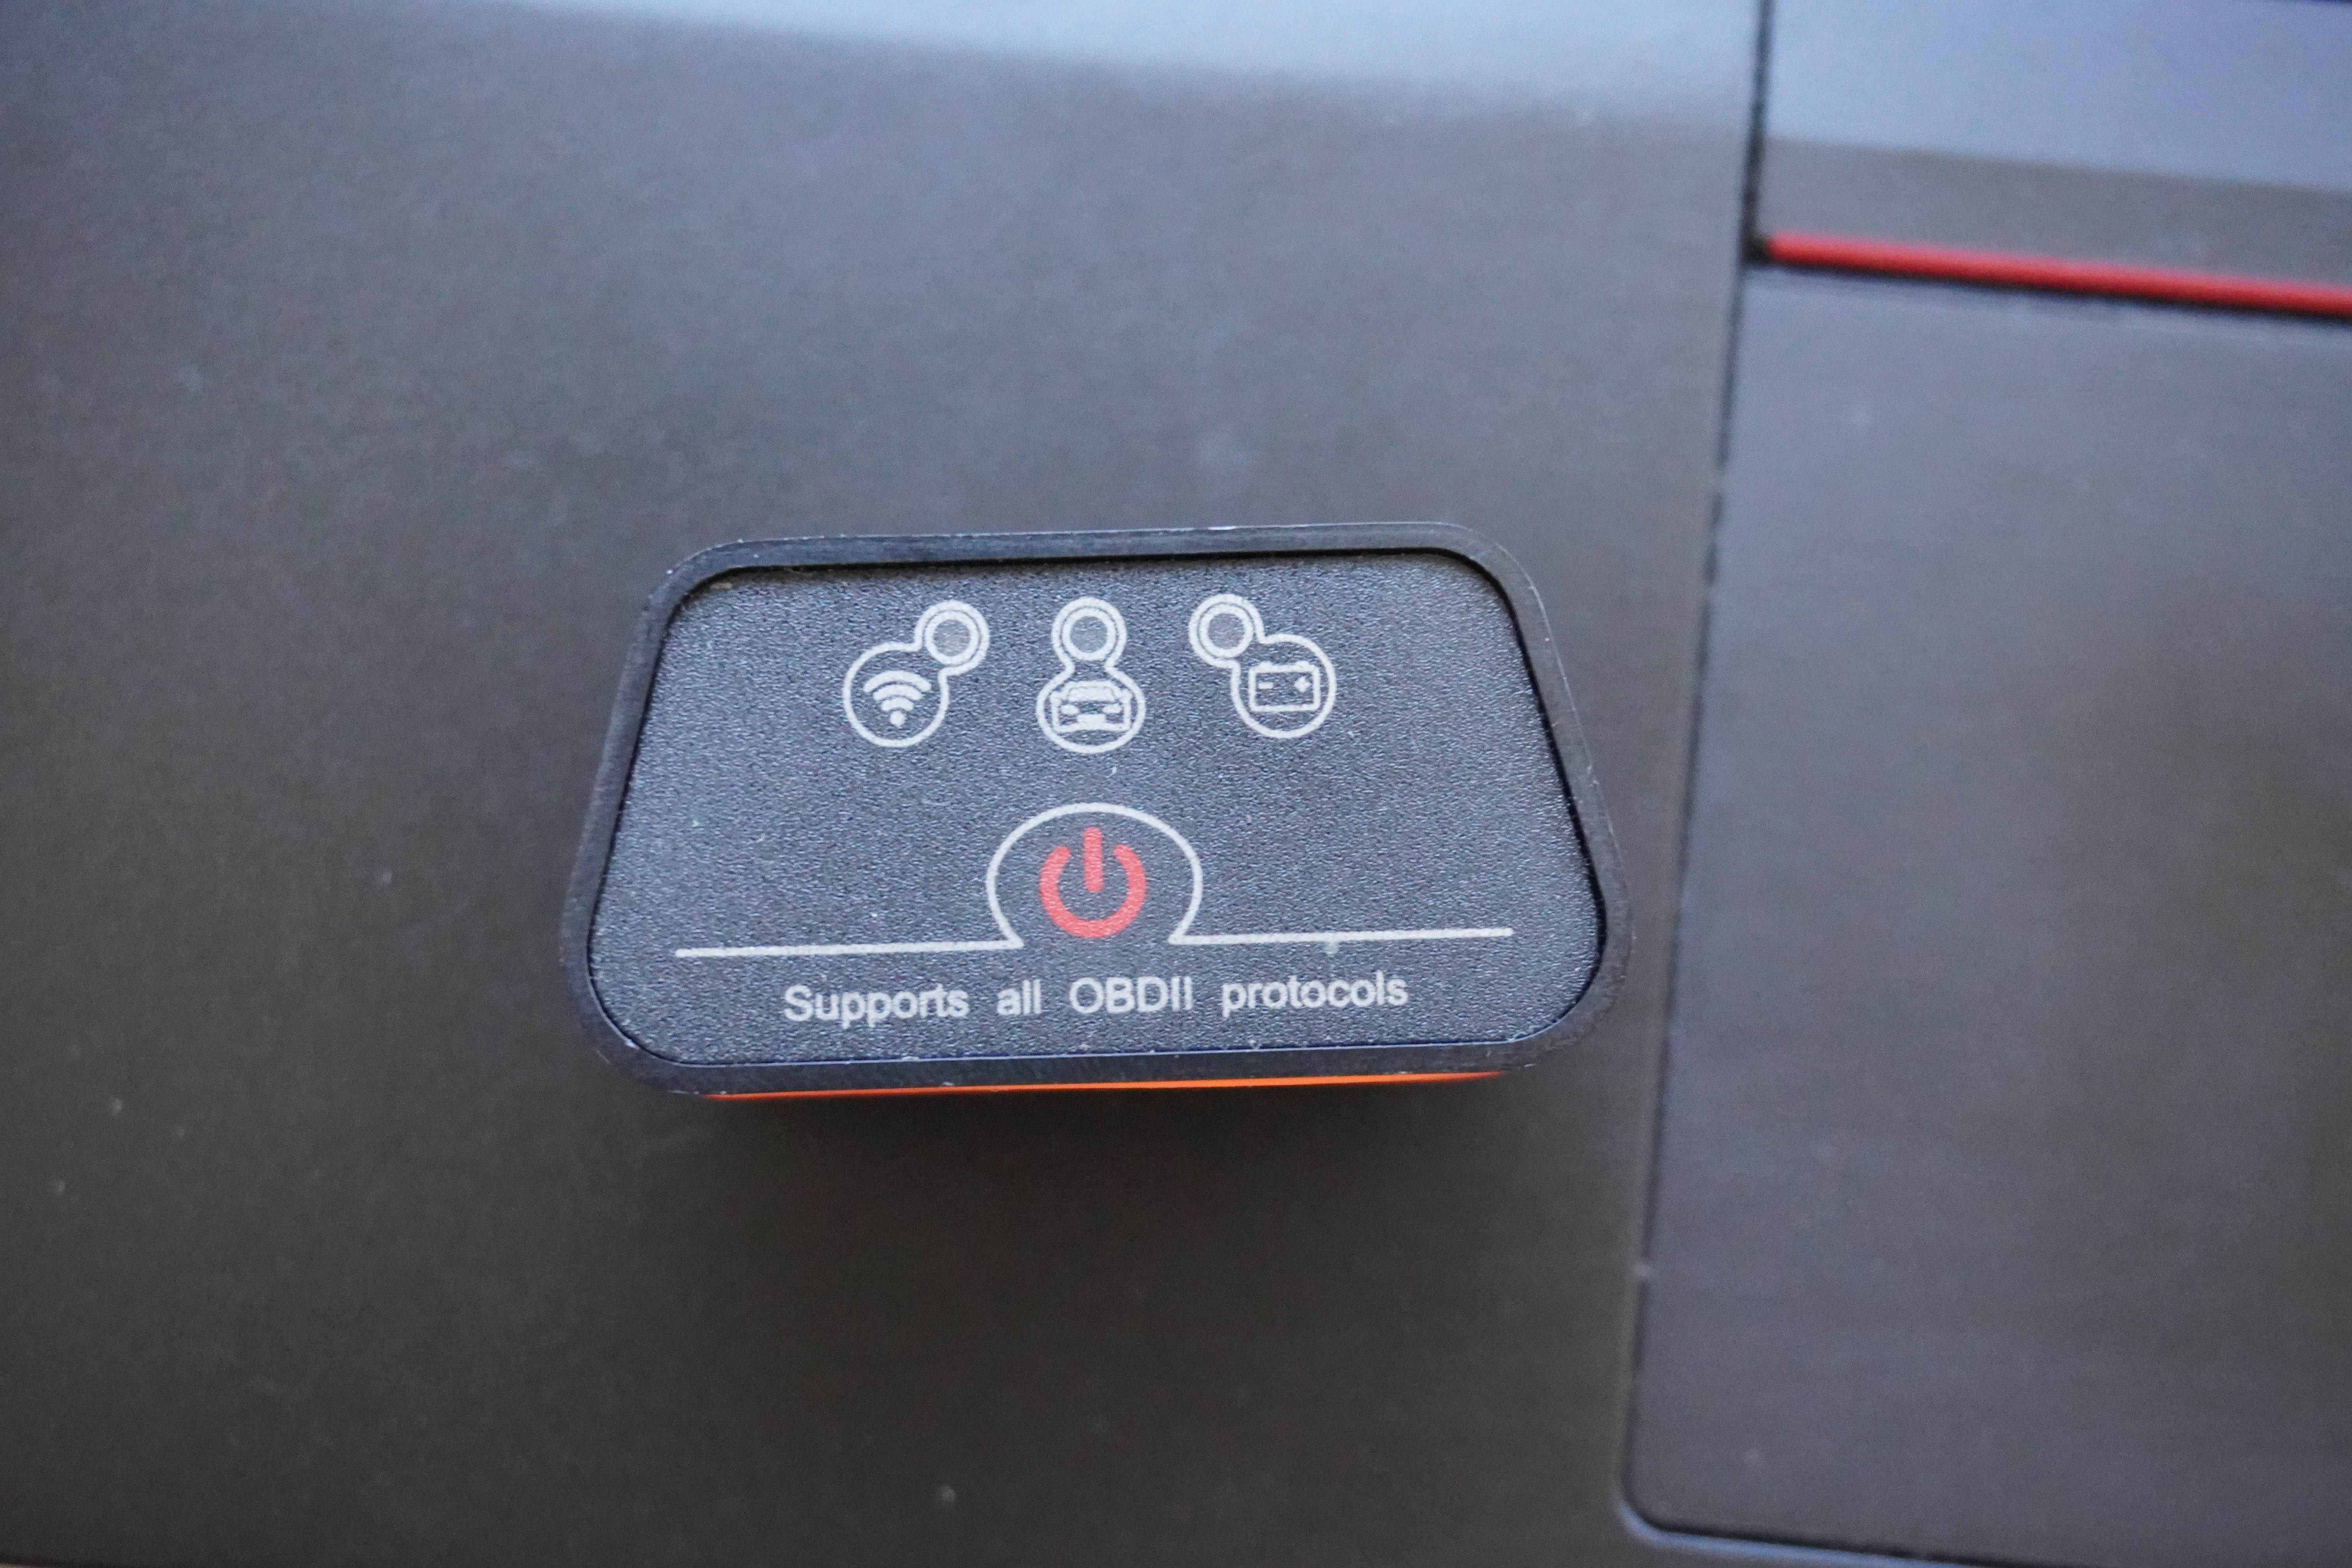
\includegraphics[width=\linewidth]{images/Hardware/obd_wifi.JPG}
        \caption{OBD WLAN-Adapter}
        \label{fig:obd_wifi}
    \end{subfigure}
    \caption{Vergleich von OBD Kabel und WLAN-Adapter}
    \label{fig:obd_comparison}
\end{figure}

Abbildung \ref{fig:obd_comparison} zeigt die beiden unterschiedlichen Systeme im Detail. Beim \ac{OBD}-II Kabel mit USB-Anschluss wird typischerweise ein Protokollcontroller wie der ELM327 oder der leistungsfähigere STN1110 eingesetzt. Diese unterstützen die gängigen \ac{OBD}-II Standards (CAN, ISO9141, KWP2000, J1850). Für die Anbindung an den PC wird zusätzlich ein USB-zu-Seriell-Wandler wie der FT232RL, CH340G oder CP2102 verwendet.  

In einem \ac{OBD}-II Bluetooth-/WLAN-Stick kommt im Kern ebenfalls ein ELM327- oder STN-Chip zum Einsatz. Dessen UART-Schnittstelle wird jedoch nicht mit USB, sondern mit einem Funkmodul verbunden, beispielsweise einem HC-05 oder RN-42 für Bluetooth Classic, einem HM-10 oder ESP32 für Bluetooth Low Energy oder einem ESP8266/ESP32 für WiFi. Beide Ansätze lassen sich somit kostengünstig mit handelsüblicher Hardware realisieren und bieten eine flexible Auswahl je nach Einsatzumgebung.

Zusätzlich kann die Diagnose durch externe Messgeräte wie Oszilloskop, Labornetzteil, Innenwiderstandsmesser oder Multimeter erweitert werden. Diese liefern wertvolle Messdaten, die über eine Sprachschnittstelle in den Diagnoseprozess einbezogen werden können. Auch wenn dieser Schritt optional ist, ermöglicht er eine noch genauere Eingrenzung und Bestätigung der Fehlerursachen.

Die Aggregation aller erfassten Informationen erfolgt in der Cloud. Dort analysieren KI-Modelle die Daten und geben konkrete Diagnoseempfehlungen mit Schritt-für-Schritt-Anleitungen aus. Das System greift dabei sowohl auf offizielle Herstellerdokumentationen als auch auf Erfahrungswissen aus Foren zurück. Gerade letzteres erweist sich als äußerst nützlich bei älteren Fahrzeugmodellen, für die Hersteller häufig nur unzureichende Informationen zu später auftretenden Problemen bereitstellen. Durch die Integration von Schwarmintelligenz aus Online-Communities können somit auch komplexe oder seltene Fehlerbilder zuverlässig erkannt werden.

\begin{figure}[h!]
    \centering
    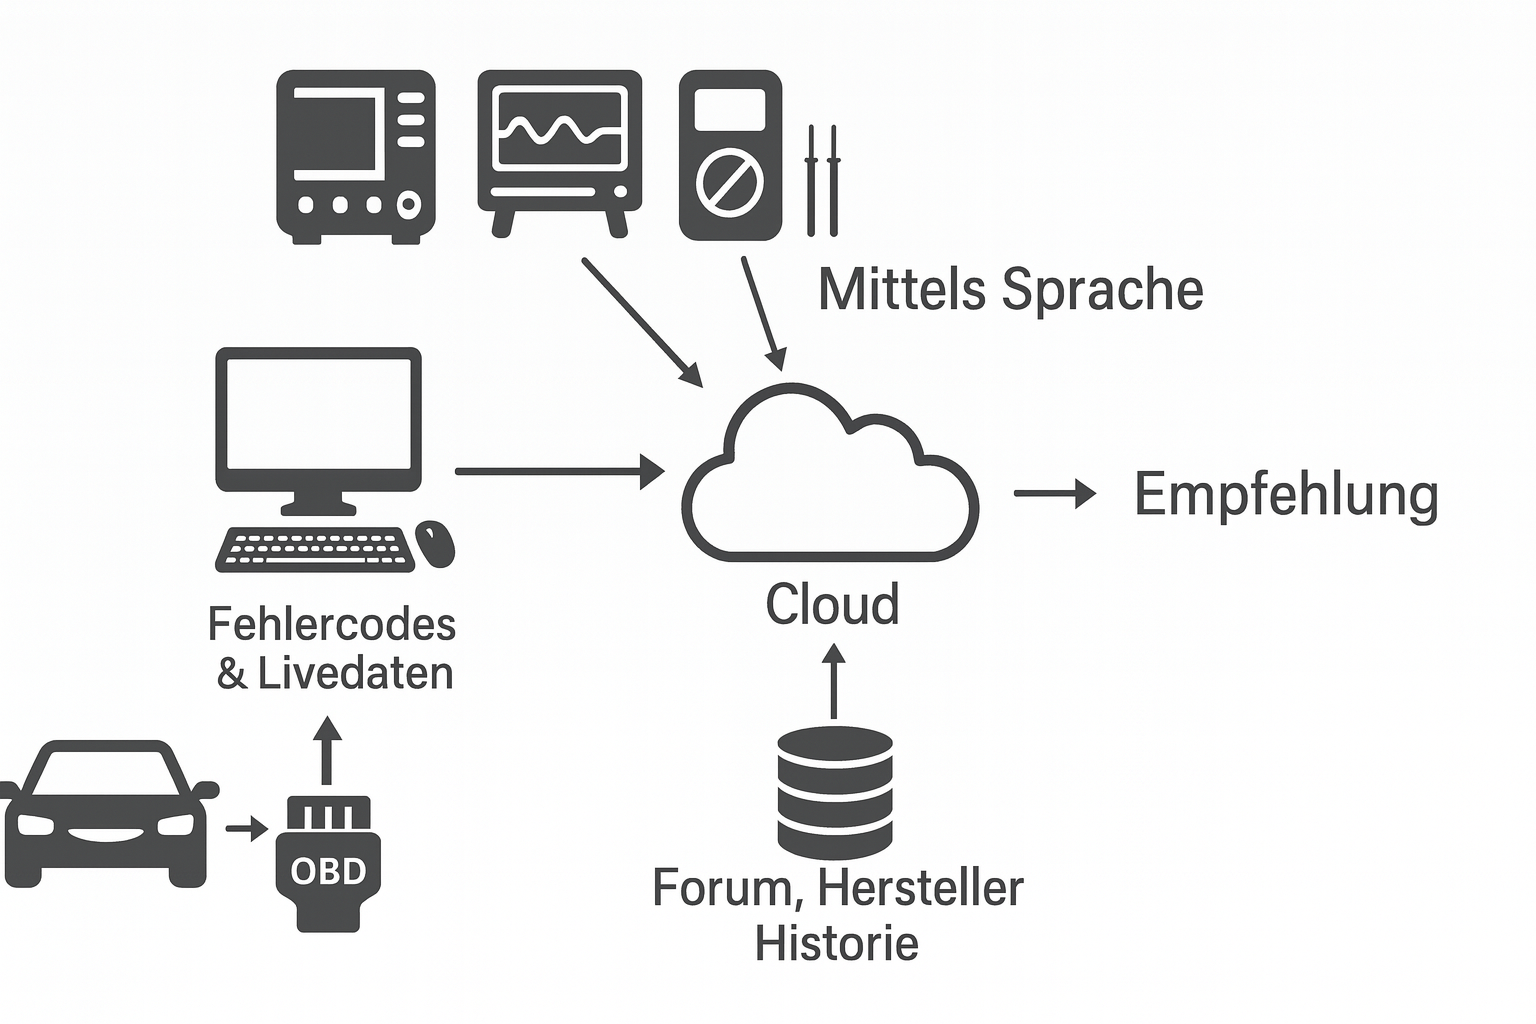
\includegraphics[width=1\linewidth]{images//Hardware/ChatGPT Image Aug 31, 2025, 04_03_25 PM.png}
    \caption{Systemarchitektur von KARL Diagnostics mit Fahrzeuganbindung, Zusatzhardware und Cloud-Komponenten}
    \label{fig:placeholder}
\end{figure}

Die Benutzeroberfläche des Diagnosesystems läuft unter Windows, sodass die Werkstatt jede handelsübliche PC-Hardware nutzen kann. Die Software wird lokal installiert und kommuniziert in Echtzeit mit der angeschlossenen Hardware sowie der Cloud.



Abbildung \ref{fig:placeholder} zeigt die Gesamtarchitektur des Systems sowie die wichtigsten Funktionsbausteine im Überblick.


\subsection{KI-Ansatz \& Erklärbarkeit}

Das \ac{KI}-System von \ac{KARL} Diagnostics bildet das Herzstück der gesamten Plattform und ist dafür verantwortlich, aus einer Vielzahl heterogener Datenquellen eine präzise Diagnose abzuleiten. Im Kern handelt es sich um ein hybrides System, das klassische regelbasierte Verfahren mit modernen Ansätzen des maschinellen Lernens kombiniert. Dadurch werden sowohl klar definierte Fehlercodes als auch komplexe, nicht unmittelbar erkennbare Muster zuverlässig erfasst und interpretiert.

Die Eingangsdaten bestehen aus standardisierten Fahrzeuginformationen über \ac{OBD}-II bzw. \ac{CAN}-Bus sowie aus zusätzlichen Messwerten externer Geräte wie Oszilloskop oder Multimeter. Diese Daten werden zunächst vereinheitlicht, zeitlich synchronisiert und in ein einheitliches Datenformat überführt. Rauschbehaftete Signale werden geglättet, relevante Merkmale extrahiert und Fehlercodes mit Metadaten wie Fahrzeugmodell, Baujahr und Herstellerinformationen angereichert. So entsteht ein strukturierter Datenstrom, der als Grundlage für die weiteren Analysen dient.

Im nächsten Schritt greift die \ac{KI}-Architektur auf mehrere Verarbeitungsebenen zurück. Für klar definierte Fehlerbilder, die in Herstellerdokumentationen eindeutig beschrieben sind, wird ein regelbasierter Ansatz verwendet. Hierdurch lassen sich deterministische Diagnosen mit hoher Transparenz erstellen. Für komplexe Sensordaten, etwa Zeitreihen von Spannung, Strom oder Temperatur, kommen hingegen neuronale Netze zum Einsatz. Besonders rekurrente Netze wie LSTMs oder moderne Transformer-Modelle sind in der Lage, Muster über längere Zeiträume hinweg zu erkennen und daraus Hypothesen über mögliche Defekte abzuleiten. Ergänzt wird dieser Ansatz durch einen semantischen Wissensgraphen, der Fahrzeugkomponenten, Fehlerursachen und Symptome miteinander verknüpft. Auf diese Weise können auch kausale Zusammenhänge modelliert werden, etwa wenn ein Spannungseinbruch nicht nur auf die Batterie, sondern auch auf die Lichtmaschine als Fehlerquelle hinweist.

Ein zentrales Merkmal von KARL Diagnostics ist die Integration externer Wissensquellen. Neben offiziellen Herstellerinformationen fließen auch Erfahrungsberichte aus Foren und technischen Blogs in das System ein. Mithilfe von Natural Language Processing werden diese Texte analysiert und relevante Muster extrahiert, die in den Wissensgraphen überführt werden. Gerade bei älteren Fahrzeugen, bei denen Herstellerdokumentationen oft lückenhaft sind, eröffnet dieser Ansatz einen entscheidenden Vorteil. Typische Fehlerbilder, die sich in der Praxis häufen, können so erkannt und in die Diagnose einbezogen werden, auch wenn sie nicht in offiziellen Handbüchern aufgeführt sind.

Die eigentliche Diagnose erfolgt über eine Hypothesengenerierung, bei der verschiedene mögliche Ursachen in Betracht gezogen und mit Wahrscheinlichkeiten versehen werden. Die Ergebnisse der unterschiedlichen Modellklassen werden in einem Ensemble zusammengeführt, wodurch sowohl Robustheit als auch Genauigkeit erhöht werden. Jede Diagnoseempfehlung wird dabei mit einem Erklärungsprotokoll versehen, das nachvollziehbar macht, welche Eingangsdaten und Wissensquellen ausschlaggebend waren. Auf diese Weise bleibt die KI nicht nur ein „Black Box“-System, sondern liefert transparent begründete Vorschläge für die Werkstattpraxis. 

Ein weiterer wesentlicher Bestandteil der Architektur ist die kontinuierliche Verbesserung. Neue Diagnosedaten aus realen Werkstätten fließen anonymisiert in das Trainingssystem ein und erweitern den Erfahrungsschatz der Modelle. Dabei werden sowohl überwachte Lernverfahren mit bestätigten Fehlerursachen genutzt als auch semi-supervised Ansätze, die unvollständig annotierte Daten einbeziehen. Um Datenschutz und Skalierbarkeit sicherzustellen, werden außerdem Methoden des Federated Learning eingesetzt, sodass sensible Kundendaten die Werkstatt nicht verlassen, während die Modelle dennoch global von Verbesserungen profitieren können.

Neben der Genauigkeit spielt auch die Zuverlässigkeit eine zentrale Rolle. Kritische Analysen, die unmittelbar für den Motorschutz relevant sind, werden lokal auf der Hardware durchgeführt, um Latenz zu minimieren. Komplexere Analysen werden in die Cloud ausgelagert, wo leistungsfähige Rechenressourcen zur Verfügung stehen. Alle Datenübertragungen sind durch Ende-zu-Ende-Verschlüsselung abgesichert, und die Cloud-Infrastruktur ist so ausgelegt, dass tausende parallele Diagnosesitzungen zuverlässig verarbeitet werden können.


\newpage

\section{Markt und Wettbewerb}
Die Kfz-Werkstattbranche in Deutschland befindet sich in einem komplexen Marktumfeld, das durch technologische Innovationen, steigende Kundenanforderungen, wachsenden Kostendruck und einen zunehmenden Fachkräftemangel geprägt ist. Anhand verschiedener statistischer Entwicklungen lassen sich zentrale Trends und Herausforderungen für die kommenden Jahre identifizieren.

\begin{figure}[h!]
    \centering
    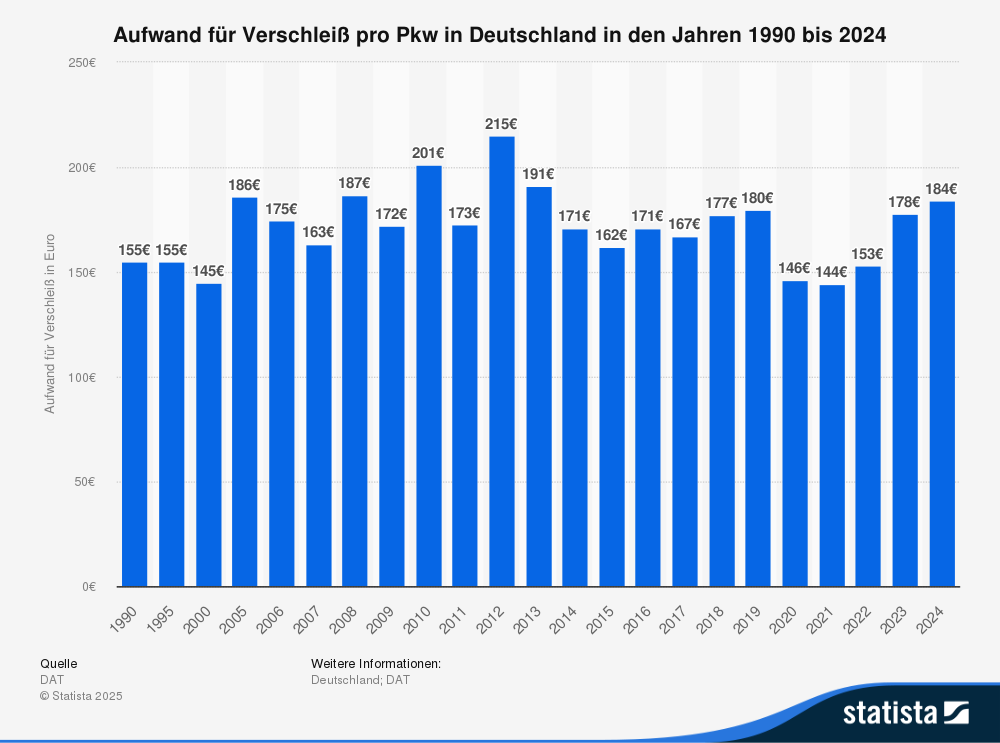
\includegraphics[width=0.75\linewidth]{images//wettbewerb/statistic_id39416_aufwand-fuer-verschleiss-pro-pkw-in-deutschland-2024.png}
    \caption{Durchschnittlicher Aufwand für Verschleiß pro Pkw in Deutschland im Jahr 1990 bis 2024 \citep{zdk2025verschleiss}}
    \label{fig:verschleiss}
\end{figure}

Ein Blick auf die Entwicklung der Verschleißkosten pro Pkw (Abb. \ref{fig:verschleiss}) in Deutschland zwischen 1990 und 2024 verdeutlicht, dass sich diese im Zeitverlauf nur geringfügig verändert haben. Nach einem kontinuierlichen Anstieg bis zum Jahr 2012, in dem mit 215 Euro ein Höhepunkt erreicht wurde, sind die Kosten in den darauffolgenden Jahren wieder gesunken und pendeln sich aktuell bei etwa 150 bis 180 Euro ein. Dies deutet darauf hin, dass Verschleißteile durch technologische Fortschritte langlebiger geworden sind und ein intensiver Wettbewerb im Ersatzteilmarkt für stabile Preise sorgt. Für Werkstätten bedeutet dies, dass das klassische Ersatzteilgeschäft nur begrenztes Wachstumspotenzial bietet und nicht mehr als Haupttreiber für Umsatzsteigerungen betrachtet werden kann. \citep[vgl.][]{zdk2025verschleiss}

\begin{figure}[h!]
    \centering
    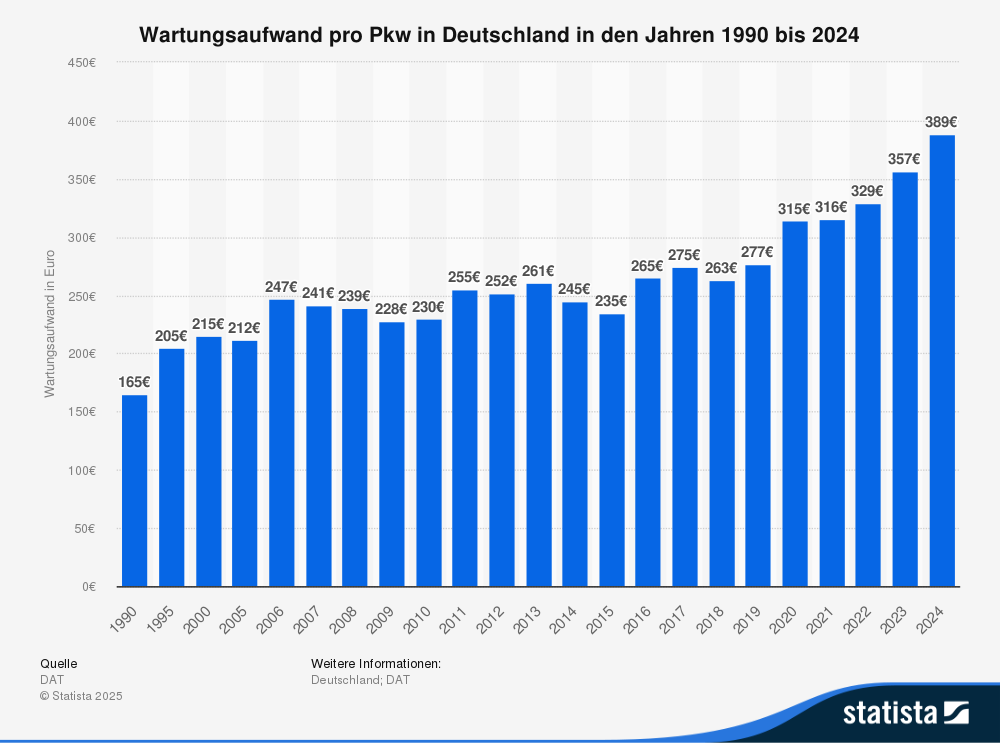
\includegraphics[width=0.75\linewidth]{images//wettbewerb/statistic_id39415_wartungsaufwand-pro-pkw-in-deutschland-bis-2024.png}
    \caption{Durchschnittlicher Aufwand für Wartung pro Pkw in Deutschland im Jahr 1990 bis 2024 \citep{zdk2025wartungsaufwand}}
    \label{fig:aufwand}
\end{figure}

Deutlich dynamischer stellt sich hingegen die Entwicklung der Wartungskosten dar (Abb. \ref{fig:aufwand}). Während diese 1990 noch bei 165 Euro pro Fahrzeug lagen, stiegen sie bis 2024 auf knapp 390 Euro an. Besonders in den letzten Jahren hat sich die Kurve stark nach oben entwickelt. Ursache hierfür ist die wachsende technische Komplexität moderner Fahrzeuge, die zunehmend mit elektronischen Steuerungen, Softwarelösungen und Fahrerassistenzsystemen ausgestattet sind. Für Werkstätten entsteht hieraus ein erhebliches Umsatzpotenzial, gleichzeitig jedoch auch ein wachsender Kostendruck auf die Kunden, die mit höheren Rechnungsbeträgen konfrontiert werden. Daraus resultiert eine zunehmende Preissensibilität, die den Wettbewerb zwischen Werkstätten verschärft. \citep[vgl.][]{zdk2025wartungsaufwand}

\begin{figure}[h!]
    \centering
    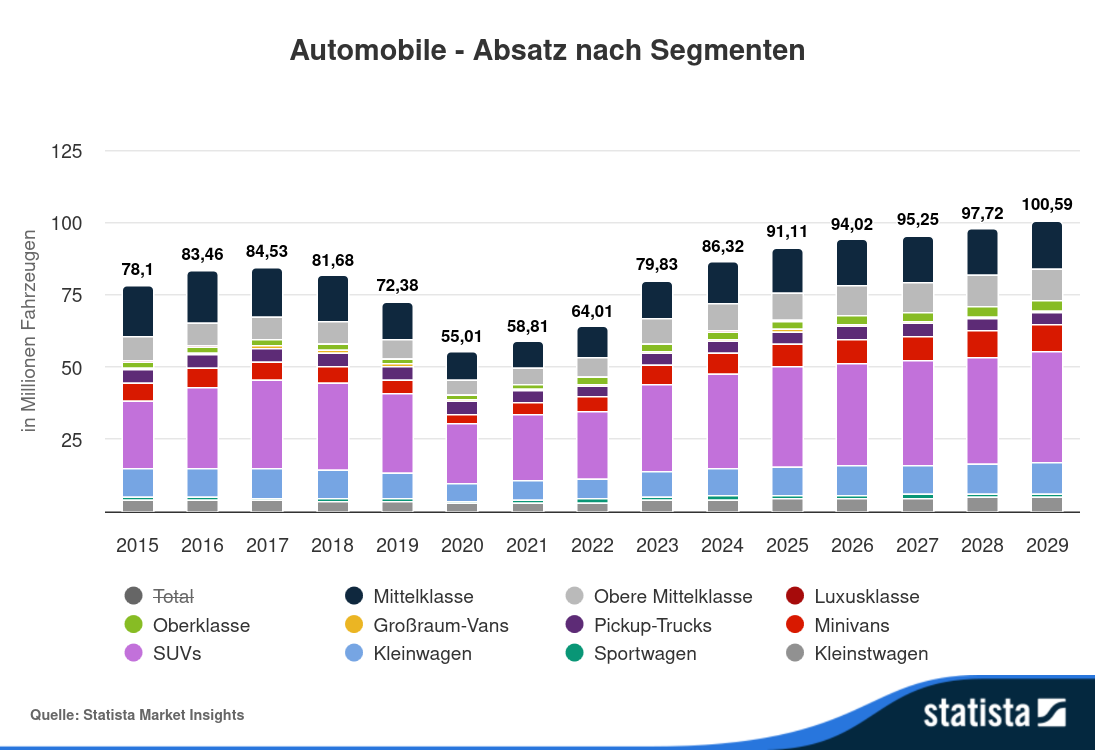
\includegraphics[width=0.75\linewidth]{images//wettbewerb/Statista-Market-Insights--Automobile-Weltweit--Absatz-nach-Segmenten.png}
    \caption{Weltweiter Absatz von Automobilen nach Segmenten im Zeitraum 2015 bis 2029 \citep[][]{statista2025automobile}}
    \label{fig:placeholder}
\end{figure}

Parallel dazu verändert sich der Automobilmarkt selbst. Die weltweiten Absatzzahlen zeigen, dass die Nachfrage nach Fahrzeugen seit dem pandemiebedingten Einbruch im Jahr 2020 wieder deutlich steigt und bis 2029 die Marke von 100 Millionen verkauften Fahrzeugen überschreiten dürfte. Auffällig ist die wachsende Bedeutung von SUVs und Fahrzeugen der Mittel- und Oberklasse. Diese Fahrzeuge sind häufig wartungsintensiver und erfordern spezialisierte Diagnosetechnik sowie regelmäßige Softwareupdates. Für Werkstätten bedeutet dies einerseits die Chance auf zusätzliche Wartungsumsätze, andererseits aber auch die Notwendigkeit, kontinuierlich in moderne Diagnosegeräte und in die Weiterbildung der Mitarbeiter zu investieren. Der Wettbewerb wird sich daher nicht mehr allein über Preis und Servicequalität entscheiden, sondern zunehmend auch über technologische Kompetenz und Spezialisierung. \citep[vgl.][]{statista2025automobile}

\begin{figure}[h!]
    \centering
    \begin{subfigure}[t]{0.7\linewidth}
        \centering
        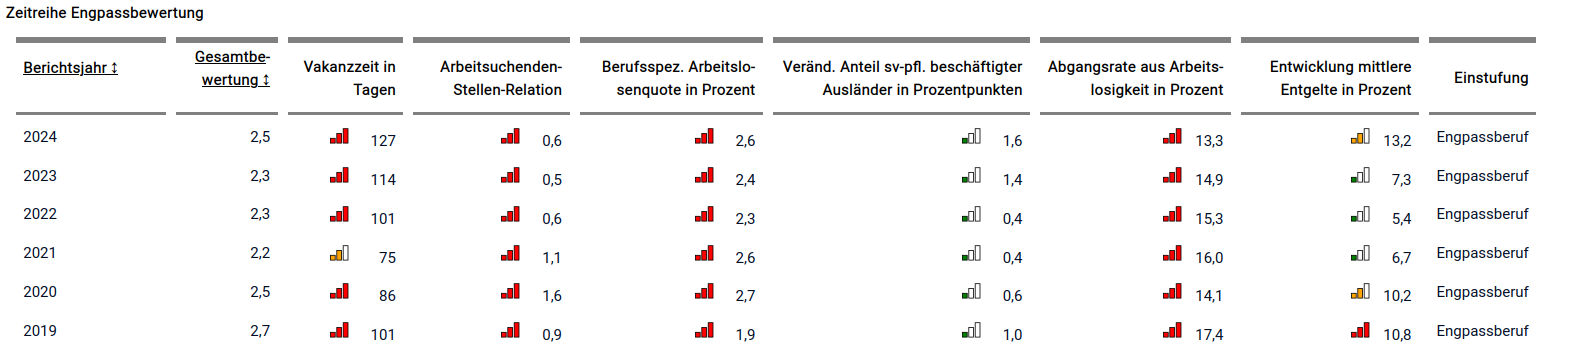
\includegraphics[width=\linewidth]{images/wettbewerb/fach_engpass.png}
        \caption{Entwicklung des Fachkräfteengpasses}
        \label{fig:fach_engpass}
    \end{subfigure}
    \hfill
    \begin{subfigure}[t]{0.26\linewidth}
        \centering
        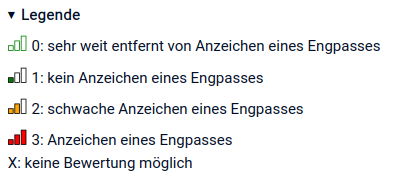
\includegraphics[width=\linewidth]{images/wettbewerb/legnde_fach.png}
        \caption{Legende Fachkräfteengpasses}
        \label{fig:legende_fach}
    \end{subfigure}
    \caption{Fachkräfteengpass in den Berufen der Mechatronik (2611) in Deutschland \citep[][]{ba2025engpassanalyse2611}}
    \label{fig:nebeneinander}
\end{figure}


Neben diesen marktwirtschaftlichen Faktoren stellt der Fachkräftemangel eine der größten Herausforderungen dar. Die Engpassbewertung für den Beruf des Kfz-Mechatronikers zeigt, dass dieser seit Jahren als Engpassberuf gilt. Die durchschnittliche Vakanzzeit bei offenen Stellen beträgt inzwischen 127 Tage, während die Relation von Arbeitsuchenden zu gemeldeten Stellen mit 0,6 sehr niedrig ist. Dies bedeutet, dass es erheblich mehr offene Stellen als verfügbare Fachkräfte gibt. Trotz steigender Bedeutung des Berufs, bedingt durch die zunehmende Komplexität der Fahrzeuge, gelingt es der Branche nicht, ausreichend Nachwuchs zu gewinnen. Für Werkstätten entsteht hier ein doppelter Druck: Einerseits wächst die technische Anforderung an die Arbeit, andererseits fehlen die qualifizierten Arbeitskräfte, um diese Nachfrage zu decken. \citep[vgl.][]{ba2025engpassanalyse2611}
\newline\newline
Zusammenfassend lässt sich feststellen, dass die Kfz-Werkstattbranche in den kommenden Jahren mit mehreren parallelen Entwicklungen umgehen muss. Während Verschleißkosten stagnieren, eröffnen steigende Wartungskosten zusätzliche Umsatzpotenziale. Gleichzeitig erfordern die Veränderungen im Automobilmarkt, insbesondere die wachsende Nachfrage nach SUVs und technisch anspruchsvolleren Fahrzeugen, höhere Investitionen in Technik und Know-how. Hinzu kommt der Fachkräftemangel, der die Wettbewerbsfähigkeit vieler Betriebe unmittelbar bedroht. Werkstätten, die langfristig erfolgreich sein wollen, müssen daher einerseits technologische Innovationsfähigkeit entwickeln und andererseits attraktive Arbeitsbedingungen schaffen, um Fachkräfte zu gewinnen und zu binden. Nur so lässt sich der steigende Kostendruck mit einer nachhaltigen Wettbewerbsstrategie ausgleichen. Gerade an dieser Stelle setzt KARL Diagnostics an. Das System unterstützt Werkstätten dabei, den steigenden technischen Anforderungen gerecht zu werden, ohne dass hierfür unverhältnismäßig hohe Investitionen in Spezialwissen oder zusätzliche Fachkräfte notwendig sind. Durch die Kombination aus automatisierter Fehleranalyse, KI-gestützter Ursachenfindung und transparenten Handlungsempfehlungen können auch weniger erfahrene Mitarbeiter komplexe Diagnosen zuverlässig durchführen. Auf diese Weise wird der Fachkräftemangel teilweise kompensiert, da die Abhängigkeit von hochspezialisierten Technikern reduziert wird. Gleichzeitig profitieren Betriebe von einer höheren Effizienz, geringeren Fehlerraten und einer schnelleren Abwicklung von Reparaturaufträgen. Ein weiterer Vorteil liegt in der kontinuierlichen Erweiterung des Systems durch Herstellerinformationen und Erfahrungsberichte aus der Praxis. So bleiben Werkstätten technologisch auf dem neuesten Stand, ohne permanent in teure Weiterbildungen oder proprietäre Diagnosesysteme investieren zu müssen. KARL Diagnostics fungiert damit nicht nur als technisches Werkzeug, sondern als strategischer Enabler, der den Spagat zwischen Kostendruck, Fachkräftemangel und steigender Komplexität moderner Fahrzeuge erleichtert und die Wettbewerbsfähigkeit langfristig sichert.

\subsection{Wettbewerbsumfeld und potentielle Konkurrenten}
Der Wettbewerb in der Kfz-Diagnose- und Werkstattsoftwarebranche ist stark fragmentiert. Auf der einen Seite stehen große, etablierte Anbieter von Diagnosetechnik wie Bosch, Hella Gutmann oder Delphi Technologies, die Werkstätten mit umfangreichen, oft herstellerspezifischen Lösungen versorgen. Diese Systeme sind leistungsfähig, erfordern jedoch häufig hohe Investitionen in Lizenzen, Hardware und regelmäßige Updates. Zudem sind sie meist komplex in der Anwendung, was die Abhängigkeit von hochqualifizierten Fachkräften verstärkt. \citep[vgl.][]{delphi2025dsdiagnosesoftware,bosch2025diagnosegeraete,hellagutmann2025diagnoseloesungen}
\newline\newline
Daneben existiert eine Vielzahl kleinerer Anbieter, die sich auf Nischenlösungen spezialisiert haben, etwa für bestimmte Fahrzeugmarken oder Teilbereiche wie Motorsteuerung, Klimasysteme oder elektrische Komponenten. Diese Tools sind oftmals günstiger, decken jedoch nur eingeschränkte Anwendungsfälle ab und bieten nicht die breite Abdeckung, die freie Werkstätten für den Alltag benötigen. Ein weiterer Wettbewerbsfaktor sind die herstellereigenen Diagnosesysteme, die von Fahrzeugproduzenten zunehmend auch für unabhängige Werkstätten zugänglich gemacht werden. Diese Systeme sind in Bezug auf Aktualität und Funktionsumfang häufig überlegen, binden die Werkstätten jedoch stärker an die jeweiligen Hersteller und schränken ihre Flexibilität im Mehrmarkengeschäft ein.
\newline\newline
Im Vergleich dazu positioniert sich KARL Diagnostics als herstellerunabhängige, \ac{KI}-gestützte Lösung, die den Spagat zwischen Funktionsbreite, Kostenkontrolle und Benutzerfreundlichkeit ermöglicht. Während traditionelle Systeme stark auf Expertenwissen angewiesen sind, verfolgt KARL einen Ansatz, der gerade weniger erfahrenen Mitarbeitern eine sichere und effiziente Fehleranalyse erlaubt. Damit unterscheidet sich KARL sowohl von den etablierten Komplettlösungen mit hohen Investitionshürden als auch von den spezialisierten Nischenprodukten, die oft nur begrenzte Einsatzmöglichkeiten bieten.





	
\section{Marketing und Vertrieb}
\subsection{Ausgangslage und Positionierung}
\ac{KARL} Diagnostics adressiert die steigende Komplexität moderner Fahrzeuge, die Verdichtung von Serviceprozessen und den anhaltenden Fachkräftemangel in Kfz-Werkstätten mit einer \ac{E2E}-Diagnoselösung, die \ac{OBD}-II/\ac{CAN}-Hardware und KI-gestützte Software verbindet (Priorisierung, geführte Prüfpläne, Teile- und Reparaturempfehlungen, perspektivisch DMS-Integration). Die Positionierung fokussiert auf präzise Erstdiagnosen, eine höhere \ac{FTFR} sowie messbare Prozesssicherheit in der Annahme und Werkstattabwicklung. Die Lösung differenziert sich durch \ac{OTA}-Updates, \ac{KI}-gestützte Fehlerpriorisierung und einen klaren Pfad zur Integration in bestehende Systeme der Werkstatt-IT \citep[vgl.][o.S.]{market-analytics-2025}.

\subsection{Business Model Canvas}
\textbf{Customer Segments}\\
\ac{KARL} adressiert primär professionelle Akteure im europäischen Kfz‑Aftermarket mit hoher Prozess- und Ergebnisverantwortung. Dazu gehören freie Werkstätten, markengebundene Servicebetriebe, Serviceketten sowie mobile Mechaniker, die markenübergreifende Diagnostik, kurze Durchlaufzeiten und verlässliche Erstbehebungsraten benötigen. Perspektivisch ist eine internationalisierte Ausweitung nach Westeuropa, Nordamerika und China vorgesehen, sobald Referenzen, Lokalisierungen und Integrationen in den Zielregionen belastbar vorliegen. Die verschiedenen Kundengruppen haben unterschiedliche Anforderungen: Kleine Werkstätten achten vor allem auf Kosten und einfache Bedienung. Werkstattketten legen Wert auf Skalierbarkeit und einheitliche Abläufe.\\

\textbf{Value Propositions}\\
Der Kernnutzen liegt in präziser, erklärbarer Erstdiagnose mit durchgängiger Prozessführung: \ac{OBD}‑II/\ac{CAN}‑fähige Hardware verbindet das Fahrzeug robust mit \ac{CARL} und \ac{KARLA}, wo \ac{KI}‑gestützte Fehlerpriorisierung, geführte Prüfpläne und Teileempfehlungen bereitgestellt werden. Das ganze System wird noch durch \ac{OTA}‑Updates ergänzt. Für Werkstätten wird damit Zeitdruck in der Annahme reduziert, die \ac{FTFR} erhöht und der Teiletausch „auf Verdacht“ durch strukturierte Ursachenanalyse ersetzt. Die Diagnosen werden nachvollziehbar, da Hypothesen, Wahrscheinlichkeiten und Begründungen transparent ausgegeben werden und jeder bestätigte Fall die Wissensbasis verbessert. Im Wettbewerb differenziert sich \ac{KARL} gegenüber teuren, komplexen Premium‑Testern und \ac{OEM}‑gebundenen Tools über Herstellerunabhängigkeit, geführte Prüfpfade, explainable AI sowie die Verbindung aus lernender Wissensbasis und pragmatischer Plug‑and‑Play‑Integration in bestehende Werkstattprozesse.\\

\textbf{Channels}\\
Der Marktzugang kombiniert direkten \ac{B2B}‑Vertrieb (Demos und Teststellungen) mit Partnerkanälen über Werkstattausrüster, Distributoren und Systemintegratoren, um Reichweite, Logistik und regionale Präsenz aufzubauen. Digitale Kanäle stützen den Funnel mit Content Marketing (Leitfäden, Fallstudien, \ac{DTC}‑Bibliotheken), Webinaren und Fachportalen. Messen und Verbandsarbeit erhöhen die Glaubwürdigkeit in konservativen Beschaffungsprozessen, während Zertifizierungen die Anwenderkompetenz sichern. Die Software wird cloudbasiert ausgeliefert und gepflegt und erhält \ac{OTA} Updates. Die Hardware wird über eine Partnerlogistik bereitgestellt. Der Rollout startet in der DACH-Region und wird anschließend auf Westeuropa ausgeweitet. \\

\textbf{Customer Relationships} \\
Wir begleiten unsere Kunden Schritt für Schritt. Von der Einführung bis zur langfristigen Nutzung erhalten unsere Kunden immer Unterstützung. Neue Kunden erhalten strukturierte Onboardings mit Schulungen um eine fehlerfreie Verwendung von KARL zu ermöglichen.Unser Customer-Success-Team sorgt dafür, dass die Software intensiv genutzt wird, Kunden als Referenzpartner gewonnen werden und Rückmeldungen direkt in die Weiterentwicklung einfließen. Dabei helfen klare Kennzahlen wie Akquisekosten, Conversion-Raten, Umsatzbindung und Kündigungsquote, um alle Phasen – von der ersten Nutzung bis zur Erweiterung – datenbasiert zu steuern. Zertifizierungen und Community-Formate sollen in der Zukunft umgesetzt werden um den Austausch von Best Practices zu fördern, denn so kann Vertrauen in KI-gestützte Empfehlungen gewonnen werden. \\

\textbf{Revenue Streams} \\
\ac{KARL} nutzt ein hybrides Modell: einmalige Hardwareerlöse aus \ac{OBD}/\ac{CAN}‑Interfaces und Zusatzsensorik sowie wiederkehrende \ac{SaaS}‑Lizenzen pro Arbeitsplatz mit gestaffelten Funktionsumfängen (z.B. Priorisierung, erweiterte Daten/Empfehlungen, Integrationen, \ac{SLA}). Ergänzende Ertragsquellen sind Schulungen/Zertifizierungen, Integrationsprojekte und Premium‑Support. Die Preispolitik ist nutzenbasiert und reflektiert Effizienzgewinne (Zeit, Erstbehebung, Teiletrefferquote) sowie die Skaleneffekte der Wissensbasis. Damit verlagert sich der Umsatzmix mit wachsender Traktion hin zu margenstarken Lizenzerlösen, während die Hardware als Enabler dient und den Geräte‑Lock‑in für stabile Nutzung sicherstellt. \\

\textbf{Key Resources} \\
Wesentliche Ressourcen sind der Diagnose‑Stack (\ac{OBD}/\ac{CAN}‑Anbindung, Datenmodelle), die Cloud‑/Mobile‑Plattform (\ac{CARL}/\ac{KARLA}), proprietäre \ac{KI}‑Modelle mit erklärbarer Ausgabenlogik und eine wachsende Wissensbasis aus realen, anonymisierten Fällen. Hinzu kommen Integrationsassets (APIs, Konnektoren), Telemetrie/Monitoring, Marken‑ und Vertriebskanäle sowie das qualifizierte, funktionsübergreifende Team (Fullstack‑Entwickler, Data Engineers/Scientist, Vertrieb, Einkauf/QS), das die Brücke zwischen Feldanforderungen und Produktinkrementen schließt. Partnerschaften mit Fertigern, Distributoren, \ac{DMS}/Telematik‑Anbietern und Cloud/Datenpartnern sind teil‑externe Ressourcen, die Lieferfähigkeit, Integrationstempo und Skalierung operativ absichern. \\

\textbf{Key Activities}\\
Im Zentrum stehen Entwicklung und Betrieb der Plattform mit kurzen Release‑Zyklen, \ac{CI/CD}, \ac{OTA}‑Update‑Mechanismen und Telemetrie gestützter Qualitätssicherung, ergänzt um Datenaufnahme, Harmonisierung, Validierung und Modelltraining samt Monitoring im Feld. Go to Market   Aktivitäten umfassen Vertrieb (Demos, Teststellungen), Partnerenablement (Co‑Marketing, Schulungen), Onboarding/Customer Success sowie Zertifizierungen zur Kompetenzsicherung. Einkauf und Qualitätssicherung managen die externe Hardwarefertigung, Zweitquellen, Prüf- und Abnahmeprozesse sowie Änderungswesen, um Serienqualität, Verfügbarkeit und Kostenstabilität sicherzustellen. \\

\textbf{Key Partnerships}\\
Für Reichweite und Liefersicherheit stützt sich \ac{KARL} auf Werkstattausrüster/Distributoren, die Zugang zum \ac{IAM}‑Netz und etablierte Logistikketten bieten, sowie auf Fertigungspartner für \ac{OBD}/\ac{CAN}‑Hardware mit geprüften Qualitätsprozessen und Zweitquellenstrategie. Integrationspartner im Bereich \ac{DMS}/Telematik und Cloud/Datenanbieter beschleunigen die Inbetriebnahme und senken Projekt‑ und Betriebsrisiken. Ausbildungs‑ und Schulungspartner sichern eine flächige Qualifizierung der Anwender. Verbandsarbeit und Messen dienen als Glaubwürdigkeits‑ und Akquisitionshebel in einem konservativen Beschaffungsumfeld und erleichtern Referenzaufbau in Zielsegmenten. \\

\textbf{Cost Structure} \\
Die Kostenstruktur umfasst F\&E für Embedded/Software/\ac{KI}, Cloud‑ und Datenbetrieb, externe Hardwarefertigung/Logistik, Go‑to‑Market (Marketing, Vertrieb, Partner), Customer Success/Support sowie Qualitätssicherung und Zuliefereraudits. Skaleneffekte in Einkauf/Fertigung und Automatisierung im Onboarding/Support (Self‑Service, In‑App‑Hilfen) senken Stück- und Servicekosten. Mit steigender Nutzerbasis verbessert sich der Deckungsbeitrag der \ac{SaaS}‑Komponente, während Hardware gezielt margenschonend als Wachstumstreiber eingesetzt wird. Regelmäßige Portfolio‑ und \ac{SLA}‑Reviews sichern die Balance aus Funktionsausbau, Betriebsstabilität und Kostenkontrolle entlang der Rollout‑Phasen (DACH → Westeuropa). \\

\subsection{Das Magische Dreieck des Geschäftsmodells}

\textbf{Ausgangspunkt und Zweck}\\
Das Magische Dreieck beschreibt ein Geschäftsmodell entlang von vier miteinander verknüpften Dimensionen: Zielkunde (Wer?), Nutzenversprechen (Was?), Wertschöpfungskette (Wie?) und Ertragsmechanik (Wert?). Änderungen an einer Ecke bedingen stets Anpassungen an den anderen, weshalb die vier Bausteine als integriertes System zu gestalten sind. Für KARL Diagnostics dient das Dreieck dazu, die herstellerunabhängige Diagnoselösung präzise auf Werkstattpraxis, skalierbare Bereitstellung und belastbare Finanzierung auszurichten, ohne den Kundennutzen aus dem Blick zu verlieren.\\

\textbf{Wer? Zielkunden}\\
Im Zentrum stehen freie und markengebundene Werkstätten, Serviceketten sowie mobile Mechaniker in DACH und Westeuropa. Die Segmentlogik unterscheidet nach Kaufkriterien: \ac{SMB}‑Werkstätten priorisieren Bedienbarkeit und TCO, Ketten benötigen standardisierte, skalierbare Abläufe. DDer Rollout startet in der DACH-Region und wird anschließend auf Westeuropa ausgeweitet. \\

\textbf{Was? Nutzenversprechen}\\
KARL liefert präzise, erklärbare Erstdiagnosen durch die Kombination OBD/CAN‑Hardware mit \ac{CARL} und mobiler App \ac{KARLA}: \ac{KI}‑gestützte Fehlerpriorisierung, geführte Prüfpläne, Teileempfehlungen, \ac{OTA}‑Updates und Offline‑Fähigkeit, eingebettet in bestehende Werkstattprozesse. Der messbare Kundennutzen umfasst höhere \ac{FTFR}, kürzere Standzeiten, weniger Teiletausch auf Verdacht sowie auditierbare Prozessqualität. Die erklärbare Ausgabe und das kontinuierliche Lernen aus anonymisierten Fällen stärken Vertrauen und Effektivität und ist ein entscheidendes Hilfsmittel in der Zeit des Fachkräftemangels. \\

\textbf{Wie? Wertschöpfungskette}\\
Die Wertschöpfung kombiniert Hardwarebeschaffung und QS, Datenaufnahme über OBD/CAN und Zusatzmessgeräte, Cloud‑Verarbeitung mit Datenharmonisierung, Modelltraining und Telemetrie‑basiertem Monitoring sowie die Auslieferung von Funktionen via \ac{CI/CD} und \ac{OTA}. Go‑to‑Market und Service werden über direkten \ac{B2B}‑Vertrieb, Partnernetze (Werkstattausrüster, Distributoren, Systemintegratoren), strukturiertes Onboarding, Schulungen und Customer Success skaliert. Integrationspartner (\ac{DMS}/Telematik) beschleunigen die Inbetriebnahme und senken Projektrisiken. \\

\textbf{Wert? Ertragsmechanik}\\
Das Erlösmodell ist hybrid: einmalige Hardwareerlöse für \ac{OBD}/\ac{CAN}‑Interfaces und wiederkehrende \ac{SaaS}‑Lizenzen pro Arbeitsplatz mit Funktions‑ und \ac{SLA}‑Staffelung. Zusätzliche Umsätze entstehen durch Schulungen, Zertifizierungen, Integrationsleistungen und Premium‑Support. Kostenblöcke liegen in F\&E (Embedded/Software/\ac{KI}), Cloud/Datenbetrieb, externer Fertigung/Logistik, Go‑to‑Market und Customer Success. Skaleneffekte in Einkauf/Fertigung sowie Self‑\\Service‑Onboarding und Telemetrie‑gestützter Support verbessern Deckungsbeiträge und verlagern den Umsatzmix hin zu margenstarken Lizenzen. \\

\textbf{Implikationen für die Gestaltung} \\
Da Optimierungen an einer Ecke stets Rückwirkungen erzeugen, muss die Roadmap auf Mehrfachanpassungen ausgelegt werden: Beispielsweise erfordert ein erweitertes Nutzenversprechen (z.B. neue \ac{KI}‑Module) sowohl zusätzliche Daten- und MLOps‑Kapazitäten in der Wertschöpfung als auch eine angepasste Preis-/\ac{SLA}‑Logik in der Ertragsmechanik. Umgekehrt bedingen neue Zielsegmente (z.B. der europäische Markt) andere Integrationen und Nachweise in der Wertschöpfung und rechtfertigen differenzierte Vertrags- und Paketstrukturen im Erlösmodell.\\

\subsection{Marketing-Mix (4P) für KARL}
\textbf{Product}\\
\ac{KARL} umfasst \ac{OBD}-II/\ac{CAN}-Hardware, eine Cloud-Applikation (\ac{CARL}) und eine Mobile App (\ac{KARLA}) für \ac{KI}-gestützte Fehlerpriorisierung, geführte Prüfpläne, Teileempfehlungen und \ac{OTA}-Updates. \\
\textbf{Price}\\
Ein hybrides Hardware-SaaS-Preismodell mit nutzenbasierter Staffelung nach Funktionsumfang, Nutzersitzen und \ac{SLA}\\
\textbf{Place}\\
Go-to-Market über DACH/Westeuropa mit direktem \ac{B2B}-Vertrieb an Werkstätten/Serviceketten/Flotten und Partnern aus dem IAM-Distributionsnetz. Software-Distribution cloudbasiert, Hardware über Partnerlogistik. Zugang zu Fahrzeugdaten und Interoperabilität sind zentrale Faktoren für Reichweite und Skalierung.\\
\textbf{Promotion}\\
Evidenzbasierter Content (Whitepaper, ROI-Cases), Präsenz bei Messen/Verbänden und digitale Lead-Generierung sind wirksam. Kundenzentrierte Demos, Teststellungen und Pilotprojekte sind entscheidend für die Akquise in einem konservativen Beschaffungsumfeld.
\section{Geschäftsmodell und Organisation}
\textbf{Wertlogik und Erlösströme}\\
\ac{KARL} verfolgt ein hybrides Modell aus Hardwareumsatz und wiederkehrenden Softwareerlösen. Die Hardware sorgt für initiale Cashflows, Gerätebindung und robuste Datenaufnahme am Fahrzeug. Die SaaS-Komponente skaliert margenstark über die wachsende Nutzerbasis und regelmäßige Feature-Updates. Ergänzende Services (Schulung, Zertifizierung, Premium-Support, Integration) erhöhen den Kundennutzen und erweitern den Umsatz je Account. Netzwerkeffekte in der Wissensbasis sowie die Datenqualität aus realen Werkstattfällen stärken im Zeitverlauf die Differenzierung und erhöhen die Qualität der Analysen. \\

\textbf{Kostenstruktur und Skalierung}\\
Die Kostenstruktur besteht aus F\&E für \ac{KI}/Software und Embedded, Produktion und Logistik der Hardware, Go-to-Market, Customer Success sowie Cloud-/Datenbetrieb. Skaleneffekte in Fertigung und Einkauf senken Hardware-Stückkosten, während Software mit geringem Grenzkostenanstieg skaliert. Ein klarer Fokus auf Automatisierung (z. B. Self-Service-Onboarding, In-App-Schulungen, Telemetriegestützte Supportpfade) reduziert Servicekosten pro Kunde und erhöht die Bruttomarge im \ac{SaaS}-Anteil auf Dauer. \\

\textbf{Kernprozesse und Qualitätsmanagement}\\
Die Produktentwicklung folgt einem agilen Rahmenwerk mit kurzen Release-Zyklen, kontinuierlichen Updates und enger Einbindung von Pilotkunden. Ein durchgängiges Qualitätsmanagement (Anforderungen, Verifikation, Validierung) stellt Reifegrad, Regeltreue und Servicefähigkeit sicher. Für die Software werden sichere Update-Mechanismen, Telemetrie und Monitoring etabliert. Für die Hardware gilt ein strukturierter Zulieferer- und End-of-Line-Testprozess mit Rückverfolgbarkeit. Dokumentierte Prüfpläne und Wissensartefakte sorgen für konsistente Servicequalität in der Praxis.\\

\textbf{Partnerökosystem und Integration}\\
Technologiepartnerschaften mit Cloud- und Datenanbietern, DMS-Anbindungen, Telematikplattformen sowie Werkstattausrüstern beschleunigen Implementierungen und reduzieren Gesamtrisiken in den Einführungsprojekten. Ein klar definierter Integrationskatalog (APIs, Konnektoren) sowie ein Zertifizierungsprogramm für Implementierungspartner sichern Qualität und Time-to-Value. Strategische Kooperationen mit Ausbildungs- und Schulungspartnern unterstützen die flächendeckende Qualifizierung der Anwender. \\

\textbf{Organisation und Steuerung} \\
Die Organisation ist in der Startphase schlank, cross-funktional und auf schnelle Iteration ausgelegt. Klare Verantwortlichkeiten in Produkt, Engineering, Operations, Vertrieb/Marketing und Customer Success werden durch Objectives and Key Results verbunden. Ein regelmäßiges Entscheidungs- und Risikoreview sichert Priorisierung und Ressourcenallokation entlang von Wachstumszielen. Governance berücksichtigt Datenschutz, IT-Sicherheit und Produktsicherheit, insbesondere im Umgang mit Fahrzeug- und Kundendaten. \\

\textbf{Internationalisierung} \\
Die Expansion verläuft phasenweise: DACH mit Fokus auf Referenzkunden und Prozessstandardisierung, anschließend Westeuropa mit lokaler Anpassung von Content, Datenabdeckung und Integrationen. Lokale Partnernetze, Sprach- und Rechtsraumadaptionen sowie abgestufte Supportmodelle sichern Kundennähe und Servicequalität. Zukünftig ist eine Ausweitung auf Nordamerika und China vorgesehen, sobald die erforderlichen Ressourcen und Partnerschaften etabliert sind. \\
  
\section{Team}
Das Unternehmerteam ist funktionsübergreifend aufgestellt, um die Entwicklung, Skalierung und Markteinführung der Gesamtlösung effizient und mit hoher Umsetzungsqualität voranzutreiben. Die Struktur ist Abbildung \ref{fig:team} zu entnehmen. Wie dort zu erkennen ist sind die Mitarbeiter in drei Teams aufgeteilt welche von den Gründern geleitet werden. Vier Fullstack-Entwickler bestehend aus einem Junior einem Intern und zwei Senior Entwicklern verantworten die Ende-zu-Ende-Softwareentwicklung für die Cloud-Applikation \ac{CARL} und die mobile App \ac{KARLA}, einschließlich Frontend, Backend, API-Design, Sicherheit und Continuous Delivery. Zwei Data Engineers (Junior und Senior) stellen Datenaufnahme, -qualität und -bereitstellung sicher, implementieren robuste Pipelines von der OBD/CAN-Quelle bis in den Cloud-Datenraum und sorgen für verlässliche Betriebsprozesse. Ein Senior Data Scientist entwickelt Diagnose- und Priorisierungsmodelle, evaluiert Modellgüte im Feld und überführt prototypische Verfahren in produktionsreife Services.
\begin{figure}[ht!]
    \centering
    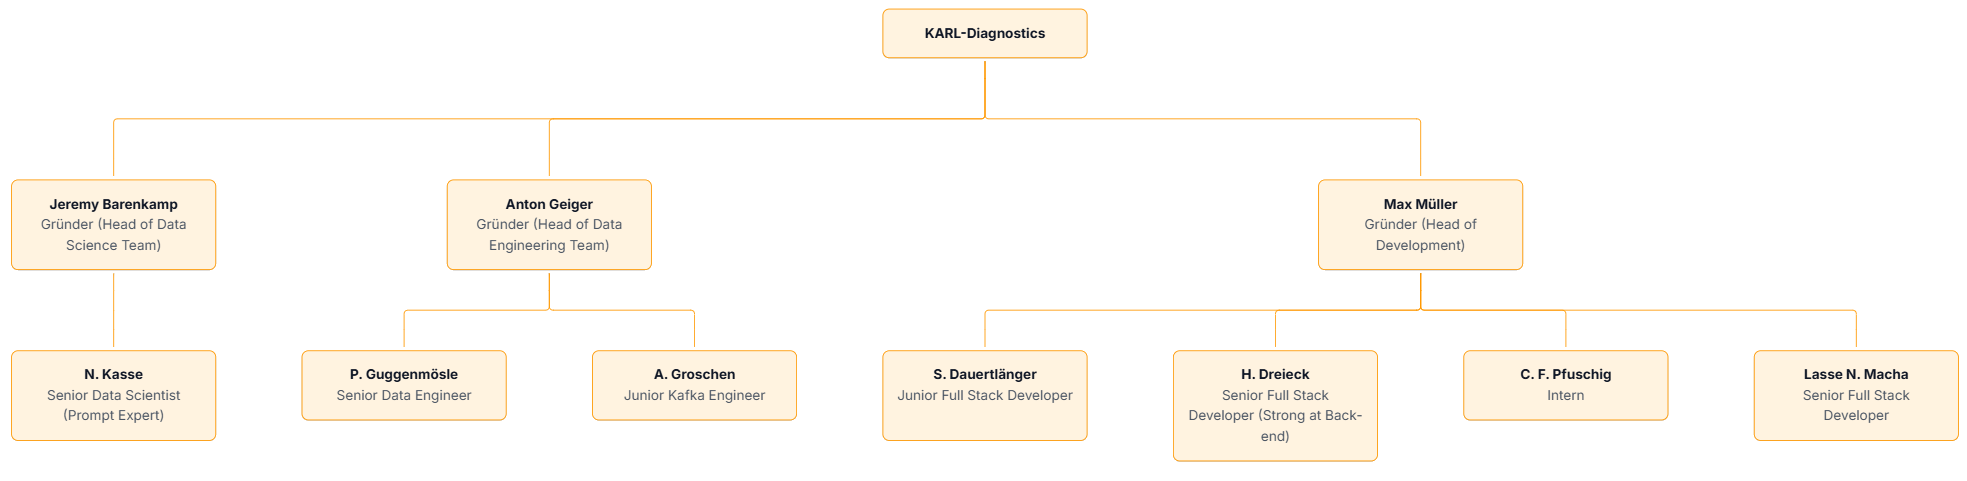
\includegraphics[width=15cm]{images/Our Organization Structure KARL-modified.png}
    \caption{Das KARL-Team}
    \label{fig:team}
\end{figure}

\textbf{Einstellungsfahrplan} \\
Ab dem 10. Monat ist eine größere Erweiterung des Teams geplant. Für den Aufbau des Vertriebs ist eine Einstellung von zwei Vertrieblern geplant. Diese sprechen Pilotkunden und Zielsegmente direkt an, koordinieren Demos, Teststellungen und kommerzielle Angebote und übernehmen die Verantwortung für strukturierte Feedbackschleifen in Richtung Produktentwicklung. Weiter ist ab dem 10. Monat eine Stelle für einen QS-Mitarbeiter geplant. Dieser soll sich primär um den Einkauf und die Qualitätssicherung kümmern. Mit wachsender Traktion werden Teamgrößen in Engineering, Sales und Support skaliert und regionale Vertriebsrollen hinzugefügt. \\

\textbf{Führung und Kultur}\\
Führung fördert Autonomie und Verantwortlichkeit, gestützt durch klare Ziele, belastbare Metriken und hohe Transparenz. Eine Lern- und Feedbackkultur beschleunigt Produktreife und Markterfolg. Kompetenzaufbau wird systematisch über Schulungen, Zertifizierungen und Communities of Practice unterstützt. Incentives kombinieren marktgerechte Vergütung mit Beteiligungsmodellen, die langfristige Wertschöpfung honorieren und die Mitarbeiter motivieren sollen. \\

\textbf{Compliance und Qualifizierung}\\
Für den Einsatz im Automotive-Umfeld werden Qualifizierungen und Standards in Entwicklung, Betrieb und Support verankert. Datenschutz, IT-Sicherheit, sichere Softwarelieferketten sowie rechtliche Rahmenbedingungen beim Datenzugriff und der -verarbeitung sind verbindlicher Bestandteil der Prozesse. Für Anwender werden Schulungs- und Zertifizierungsprogramme etabliert, die Qualität und Sicherheit in der Anwendung fördern sollen.
    \section{Realisierungsplan}

\textbf{Iterative Entwicklung des fertigen Produktes} Q1 J1 - Q1 J2 \\
Als erste Aktion f\"ur KARL Diagnostics l\"asst sich die Entwicklung eines \ac{MVP} anf\"uhren, welches die Software- und Hardware-Komponenten umfasst. Bei der Hardware geht es dabei vor Allem um die Auswahl des Ger"ateumfangs und der Partnerhersteller. Softwareseitig muss angefangen werden die Datenquelle zu erheben und diese an eine Suchengine angebunden werden. Dannach muss die Kommunikation der Ger"ate mit der Karla Cloud implementiert werden. Diese Entwicklungen erfordert eine umfangreiche Anstrengung, sodass an diesen Aufgaben alle Data Scientist, Engineers und Sotwareentwickler gebunden sind. Die Hardware muss dabei in der Lage sein, Sensordaten \"uber die \ac{OBD}-II-Schnittstelle zu erfassen und diese Daten an die IT-Infrastruktur zu senden und zu empfangen.
Das Ziel ist es dabei am Anfang jedes Quartals zehn prototypische Ger\"ate zu verkaufen und diese testweise an Kunden auszuliefern, um erstes Feedback zu sammeln. Die ersten Kunden sollen dabei sehr g"unstige Konditionen erhalten und f"ur das Abo bis zum Markteintritt nichts bezahlen m"ussen. Softwareseitig erleben diese immer den aktuellen Entwicklungsstand der CARLA Cloud mit und erhalten aktuell entwickelte Features.

Auf Basis des Kundenfeedbacks aus der ersten Phasen werden nun Optimierungen und \glqq Should-Have \grqq-Funktionen umgesetzt. Dazu geh\"oren beispielsweise Verbesserungen am User Interface, ein ergonomischeres Ger\"atedesign, der Anschluss weiterer Datenquellen, optimierung der Suchengines oder \ac{KI} Modelle oder die Implementierung automatisierter Backups. Parallel zur Weiterentwicklung an der Softwareinfrastruktur werden weitere Pilotkunden f\"ur die fr\"uhen Verkaufsmonate ausgew\"ahlt und diese mit unseren Produkten zu geringen Preisen versorgt. Diese geben dann durch ihre Erfahrungen in den Pilotprojekten bis zur fertigen Produktentwicklung wichtige Informationen und Anforderungen an unser Entwicklungsteam weiter, sodass die Entwicklung des fertigen Produktes sich bestm"oglich an die Kundenanforderungen orientiert und sich als iterativer Prozess gestaltet. Unmittelbar vor dem offiziellen Markteintritt erfolgen umfangreiche Investitionen, da Produktionskapazit"aten geschaffen, Lager gebaut und betriebswirtschaftlich orientierte Mitarbeiter wie Eink"aufer oder Vertriebler eingestellt werden. 


\textbf{Markteintritt} Ab Q1 J2 \\
Sobald der Meilenstein der Entwicklung eines verkaufsf"ahigen Produktes erreicht ist, kann der Markteintritt erfolgen. Durch gezieltes Direktmarketing sollen erste Werkst\"atten als Kunden in Deutschland gewonnen werden wof"ur gr"o"sere Summen des Budgets verwendet werden sollen. Der Markteintritt in den deutschen Markt nach 12 Monaten h"angt dabei von dem Feedback der Kunden auf den ersten Prototypen und der Entwicklungsgeschwindigkeit der Mitarbeiter ab d"urfte aber mit den 6 Teammitgliedern, welche allein f"ur die Entwicklung verantwortlich sind, realistisch sein. Langfristige Marketingma"snahmenen k"onnten ebenfalls Beteiligungen im Rennsportserien sein. \\

Unsere langfristige Wachstumstrategie sieht eine internationale Expansion vor, da der Nutzen unseres Produkts mit einer größeren, globalen Wissensbasis steigt. Ein späterer Schritt könnte – sofern die Marktlage und das Risikoprofil es erlauben – auch die Ausweitung auf den \ac{B2C}-Markt sein. Der Fokus liegt jedoch zunächst klar auf dem erfolgreichen Markteintritt und Wachstum im deutschen Heimatmarkt. Daher w"are ein Eintritt in den \ac{B2C} Markt erst nach etwa 2 oder 3 Jahren nach Markteintritt in unserer Planung. Visusalisiert ist dieses Vorgehen für die ersten 5 Quartale in der mehrdimensionalen Roadmap \textbf{Abb. \ref{fig:roadmap}}.



\begin{enumerate}
    \item Entwicklung des \ac{MVP}s (Hard- \& Software) (Q1 J1)
    \item Feedback einholen durch Pilotprojekte (Q1, Q2, Q3 J1)
    \item Optimierung bisherigen Protoypens (Q1, Q2, Q3, Q4 J1)
    \item Durchf"uhrung von Pilotprojekten mit Pilotkunden (Q2, Q3 J1)
    \item Beginn mit den Marketingaktivit"aten (Q4 J1)
    \item Steigerung der operativen Teamkapazit"at (Q4 J1)
    \item Markteintritt DT (Q1 J2)
    \item Durchf"uhrung von fl"achendeckenden Marketingaktivit"aten (Q1 J2)
    \item Markteintritt global (noch nicht definitert)
    \item Expansion auf Consumer Markt (noch nicht definitert)
\end{enumerate}


\begin{figure}[ht!]
    \centering
    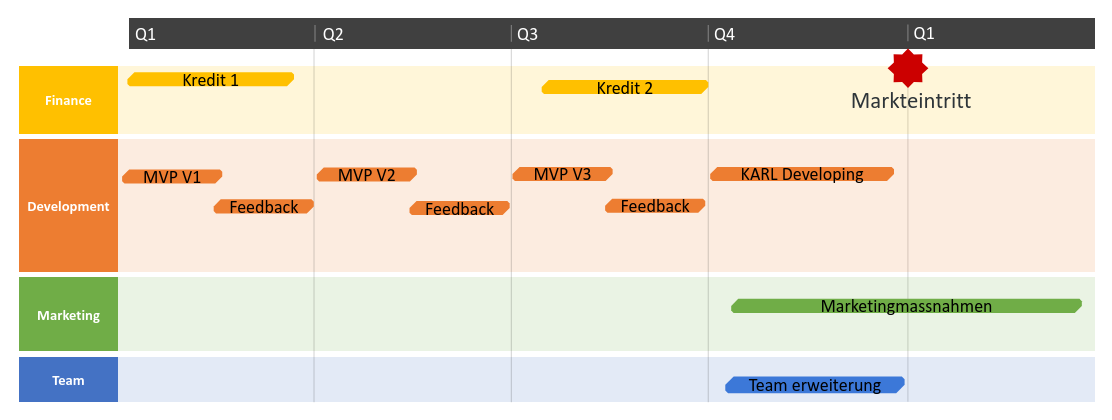
\includegraphics[width=15cm]{images/Roadmap.png}
    \caption{Roadmap f"ur KARL Diagnostics - ersten 5 Quartale}
    \label{fig:roadmap}
\end{figure}

\newpage

\section{Chancen und Risiken}

F"ur die Einordnung der Chancen und Risiken und Vorstellung der Strategien wie die Chancen ergriffen und die Risiken vermieden werden k"onnen wurde eine SWOT Analyse erstellt. Zur besseren "Ubersicht werden die Chancen und Risiken f"ur einige Unterkategorien vorgestellt und im Nachheinein erkl"art wie auf diese reagiert werden k"onnte.

\subsection{Produkt}
\textbf{Chancen} \\
Hinsichtlich des Nutzens und der Qualit\"at unseres Produktes l\"asst sich ein durch unser Gesch"aftsmodell bedingter \textbf{Netzwerkeffekt} feststellen: Der Nutzen f\"ur unsere Kunden steigt, je mehr Werkst\"atten die Plattform nutzen und ihr Wissen teilen. Es besteht also die Chance dass sich KARL als quasis Standard langfristig etabliert und diese Entwicklung w"urde einen langfristigen Nutzen des Produktes und unserer Plattform  gew\"ahrleisten. So entsteht durch den \glqq Lock-in-Effekt\grqq ein Zyklus, der neue Kunden anzieht, wodurch wiederum die Qualit\"at des Produktes durch neue Daten steigt.

Durch das Interesse der Automobilhersteller eine m"oglichst einfache und effiziente Wartung ihrer Fahrzeuge zu erm"oglichen, liegt es gleichm"a"sig im Sinne der Automobilhersteller, dass ihre Autos bestm\"oglich repariert werden k\"onnen. Daher besteht die Chance die Qualit"at unseres Produktes zu verbessern, indem die \textbf{Automobilhersteller es uns erlauben ihre Daten in unsere Datenbank} zu integrieren. So kommen wir an sehr viele h"ochstqualitative Daten.

\textbf{Risiken} \\
Ein Risiko liegt im explorativen Charakter des Produktes. Explorativ sind dabei nicht die zu verkaufende Hardware, wie Diagnoseger\"ate mit \ac{OBD}-II-Schnittstelle oder Oszilloskop an sich, da Hersteller wie Bosch solche Systeme bereits anbieten. Jedoch ist es nicht sicher, dass die \textbf{Datenqualit\"at} der Informationen aus Foren oder Werkst"atten zu verl\"asslichen, hochqualitativen Ergebnissen f\"uhren kann, da es keine vergleichbare Produkte gibt. \\
%Auch ist nicht garantiert, dass weitere Daten der Autowerkst"atte in Datenschutzkonformer Form ebenfalls wichtige Informationen unserer Datenbasis hinzuf"ugen.
% \textbf{Reaktion} \\
% % Au\ss erdem zeigen \ac{RAG} Beispiele sowie das Training von \ac{LLM}-Modellen auf \"ahnlich unstrukturierten Daten positive Resultate, weshalb angenommen werden kann, dass wichtige Informationen extrahiert werden k\"onnen. 
% Moderne Datenplattformen generieren vor Allem ihren Mehrwert dadurch Datenquellen logisch zu verkn"upfen und daraus wertvolle Informationen zu generieren und die Suche zu optimieren. Daher m"ussten in dem Fall Features wie eigenst"andige Datenverkn"upfung und Aufbauen von Datenkatalogen und \ac{KG} unterst"utzt werden, um das maximale Potenzial aus den Daten zu erhalten. Da die Foren nur einen Teil der Datenbasis ausmachen werden kann verst"arkt auf andere Datenquellen, wie den Mitschriften der Werkst"atten gesetzt werden oder gar Daten von den Automobilherstellern direkt gekauft werden.


\subsection{Markt}
\textbf{Chancen} \\
Chancen, dass sich f"ur KARL Diagnostics ein gro"ser Markt auftut ist durch die einfache \textbf{"Ubertragbarkeit des Gesch"aftsmodells} auf andere Branchen gegeben. So gibt es in der Luft- oder Schiffahrtsbranche \"ahnliche Voraussetzungen, und KARL Diagnostics k\"onnte k\"unftig in diese expandieren, was den potenziellen Markt vergr\"o\ss ert. 

Aktuelle Trends, wie die Entwicklung neuer Antriebstechnologien (z. B. Wasserstoff- und Elektroautos), haben keinen negativen Einfluss auf unser Gesch\"aftsmodell. Im Gegenteil: Sie erfordern, dass \textbf{neues Know-how in den Werkst\"atten etabliert} werden muss. Hierbei unterst\"utzt KARL Diagnostics, indem es deutschen Werkst\"atten erm\"oglicht, Wissen aus der ganzen Welt f\"ur einen besseren und schnelleren Kundensupport zu nutzen. Der Erfolg und der Nutzen des Produktes h\"angen daher nicht vom Automobilmarkt in Deutschland oder aktuellen lokalen Problemen ab, sondern vom globalen Wissen ab. 

Generell ist der Trend in der Automobilindustrie, dass Autos und ihre Technologie immer komplexer durch einen gr"oseren Funktionsumfang werden, weshalb Werkst\"atten durch die immer \textbf{schnelleren Updates nicht mehr mithalten} k\"onnen. Verfolgt sich dieser Trend weiter so sind Smarte Produkte, wie das von KARL Diagnostics unumg"anglich f"ur Werkst"atten zu benutzen. \\

Weitere Trends wie Elektroautos versprechen \textbf{l\"angere Lebenszyklen und Zuverl\"assigkeiten} der Fahrzeuge, weshalb diese zwar seltener, aber dennoch f\"ur Reparaturen in die Werkstatt kommen m\"ussen. Neuwagen werden voraussichtlich seltener ben\"otigt, da Elektromotoren und Batterien langlebiger sind. Somit ist zu erwarten, dass die Wertsch\"opfung in der Werkstatt durch Reparaturen in Zukunft steigen und der Markt auch trotz Elektromobilit\"at wachsen wird.

Hinzu kommen Trends wie der Fachkr"aftemangel oder das steigende Durschnittsalter der Autos und der steigende Anteil "alterer Autos in Deutschland nach, die immmer mehr Werkst"atte in effizientere Arbeit fordert \citep[][]{Statista-Auto-Alter}.

\textbf{Risiken} \\
\textbf{Over-the-Air-Updates}, die vor allem durch Tesla vorangetrieben werden, sind insofern gef\"ahrlich, als Autos zuk\"unftig nicht mehr unbedingt in die Werkstatt m\"ussen, um Softwarefehler zu beheben. M\"angel, die rein softwaretechnisch behoben werden k\"onnen, werden nicht mehr in der Werkstatt gefixt. Somit w\"are das Produkt von KARL Diagnostics in diesem Anwendungsfall nicht n\"otig.

Ebenfalls riskant kann sein, dass Werkst\"atten gar nicht das Bed\"urfnis sehen, \textbf{Daten international und mit anderen Werkst\"atten zu teilen}. Damit s\"anke der Markt, da die Netzwerkeffekte nicht mehr so stark wirken. Gro\ss e Werkst\"atten wie ATU k\"onnten es negativ sehen, wenn andere Werkst\"atten von ihrem Wissenspool profitieren, da diese in einem Wettbewerbsverh\"altnis zueinander stehen.


% \textbf{Reaktion} \\
% Over-the-Air-Updates k\"onnen nur Software-Probleme beheben. Aufgrund physischer, mechanischer und mechatronischer Probleme an Autos wird immer eine Werkstatt ben\"otigt. Da wir kein reines Softwareprodukt anbieten, ist KARL Diagnostics nicht unmittelbar von diesem Risiko betroffen.

% Hinsichtlich des Risikos, dass Werkst\"atten ihre Daten nicht teilen wollen, kann eine Antwort eine kluge Wahl der Implementierung und des Roll-outs sein. Es ist anzunehmen, dass kleine Werkst\"atten weniger Probleme damit haben, Informationen zu teilen. Daher sollten diese als erste Kunden akquiriert werden. Langfristig profitieren viele kleine Werkst\"atten davon, und der Druck auf gro\ss e Werkst\"atten wie ATU wird so gro\ss, dass der Grenznutzen des Produkts die Risiken des Datenteilens \"ubertrifft. Au\ss erdem sind Optionen von Belohnungssystemen (Rewards) wie Preisnachl\"asse m\"oglich, wenn Werkst\"atten Daten teilen.

\subsection{Rechtliche Aspekte}
\textbf{Risiken} \\
Ein gro\ss es rechtliches Risiko liegt in der Nutzung von \textbf{Web Scraping und Text Data Mining}-Ans\"atzen f\"ur die Erstellung unserer Datenbasis. Einige Foren verbieten die Nutzung von Data-Mining-Methoden aktuell explizit in ihren Nutzungsbedingungen.

% \textbf{Reaktion} \\
% W"urde f"ur unseren Anwendungsfall die rechtliche Grundlage f"ur das WebScraping fehlen m"ussten anfangs die Preisstrategie angepasst werden sodass viele Werkst"atte eher bereit sind ihr Wissen zu teilen und somit prim"ar die Datenbasis gef"ullt wird.

\subsection{Wettbewerber}
\textbf{Chancen} \\
Ein gro\ss er Vorteil ergibt sich aus der \textbf{Komplexit\"at des Nachahmens}, sobald ein umfangreicher Datensatz und ein umfassendes Wissen aufgebaut wurden. Dies liegt vor allem an den bereits angef\"uhrten Netzwerk- und Lock-in-Effekten. F\"ur neue Wettbewerber wird es zunehmend schwieriger, Werkst\"atten zu \"uberzeugen, sich auf einer neuen Plattform anzumelden. \\
\textbf{Risiken} \\
Ein Risiko ergibt sich durch potenzielle Konkurrenz von Automobilherstellern. Wie bereits erw\"ahnt, haben diese ebenfalls ein Interesse an der Funktionalit\"at unseres Produktes. Dementsprechend k\"onnten Automobilhersteller eigene, konkurrierende L\"osungen entwickeln, die eine h\"ohere Datenqualit\"at aufweisen, da sie direkt auf ihre eigenen, propriet\"aren Daten zugreifen k\"onnen. \\
% \textbf{Reaktion} \\
% Wenn dieser Fall eintreten w"urde muss die Unabh"angigkeit der Hersteller als \ac{USP} stark in den Blick geholt werden. Die Marketingaktivit"at muss sich vor Allem auf unabh"angige Werkst"atten beschr"anken und diesen Vorteil in den Marketingaktivit"aten hervorheben. 

\subsection{Marketing \& Vertrieb}
\textbf{Chancen} \\
Durch die erfolgreiche Umsetzung der Strategie ist es denkbar, dass sich in einigen Jahren eine Art \textbf{Monopolstellung \& Abh"angigkeit} ergibt. In diesem Fall kann die Preispolitik relativ frei gestaltet werden.

\textbf{Risiken} \\
Wenn, wie im Realisierungsplan vorgesehen, auch internationale M\"arkte wie China bedient werden sollen, besteht ein Risiko in der Preispolitik. Der Mehrwert, den Werkst\"atten durch das Produkt von KARL Diagnostics in Form von \textbf{Personalkosteneinsparungen} erzielen, kann in China andere Ausma\ss e annehmen als in Deutschland, da die Personalkosten dort geringer sind. Somit besteht das Risiko, dass eine Expansion in solche M\"arkte die gesamte Marge schm\"alern k\"onnte.

Erg\"anzend dazu ist die geplante Expansion in den \ac{B2C}-Markt riskant, da dies einen \textbf{Zielkonflikt} zwischen den Werkst\"atten und KARL Diagnostics hervorrufen k\"onnte. Das Produkt w\"urde Endkonsumenten zu einer vereinfachten Selbstreparatur bef\"ahigen, wodurch weniger Gesch\"afte f\"ur die Werkst\"atten anfallen w\"urden. \\

% \textbf{Reaktion}\\
% Eine Reaktionen darauf ist es die Preise in den L"andern so anzupassen, dass sie im dortigen Markt ad"aquat sind. Dabei k"onnte es beispielsweise sinvoll sein die Preise des Ger"ates unter Herstell oder Einkaufspreise zu setzen, da unser Gesch"aftsmodell sich prim"ar durch die Abonement Geb"uhren finanzieren soll. Auf dem \ac{B2C} muss dann die Datenbasis soweit reduziert werden, dass keine Informationen der Werkst"atte an die Privatkunden gelangt.


\subsection{Finanzierung}

\textbf{Risiken} \\
Ein Risiko des aktuellen Gesch"aftsmodells ist die kapitalintensive Eigenschaften der Branche dadurch, dass Konkurrenten wie Bosch bereits etablierte Player sind und um viel mehr finanzielle Mittel und Know How verf"ugen als wir. Deshalb ist zu erwarten dass es an umfangreichen Investitionen bedarf um die Qualit"at der Soft- und Hardware auf ein markt"ubliches Niveau zu hieven.
Somit ist ein Risiko, dass sich unser Unternehemn zunehmend verschuldet und nicht rechtzeitig profitabel wird bis die Verbindlichkeiten, die am Anfang ben"otigt werden abbezahlt sind. \\
\textbf{Chancen} \\
Dies ist jedoch auch eine Chance, da es Nachahmungseffekte reduziert und wir als First Mover am Markt ein strategischen Vorteil davon h"atten. \\

% \textbf{Reaktion} \\
% Da vor Allem der Aufbau einer Produktion der Ger"ate, wie die \ac{OBD} II Diagnoseger"ate kapitalintensiv ist und die Software den \ac{USP} bei unserem Unternehmen ausmacht, ist die Reaktion darauf, dass geplant wird die Hardware, die wir verkaufen direkt fertig eingekauft werden. Somit sinkt die Marge gegen"uber den Konkurrenten jedoch sind die Abonements die weitere Einnahmequelle die durch die Nutzung der Cloud Software eingenommen werden ohne hohe Investitionskosten wie Lager oder Produktionsanlagen verbunden. Dies zeigt auch der im sp"ateren Verlauf des Business Plans vorgestellter Vergleich zwischen den Umsatz Anteilen am Markteintritt und zwei Jahre sp"ater \textbf{Abb. \ref{fig:umsatzvergleich}}. \\ 
\subsection{Strategische Ausrichtung}
Die strategische Ausrichtung des Geschäftsmodells basiert auf einer umfassenden SWOT-Analyse, aus der die entsprechenden SO, ST, WO und WT Strategien abgeleitet werden. Angesichts des umfangreichen Marktpotenzials und der umfassenden Möglichkeiten wird die SO-Strategie  als primäre Kernkomponente verfolgt. Die Umsetzung dieser Strategie erfolgt durch die Schaffung einer breiten, herstellerunabhängigen Wissensplattform, die als wesentlicher Wettbewerbsvorteil dient und es einer Vielzahl von Werkstätten ermöglicht, das Produkt unabhängig von ihren spezifischen Ausrüstungsherstellern zu nutzen und dabei die Nutzer langfristig an einen zu binden, sodass die Plattform stetig an Benutzerzahlen w"achst. Fehlendes Know soll mit dem Eingang langfristiger Kooperationen wie die Einbindung durch die Pilotkunden aufgebesser werden.


Ergänzend dazu ist eine Marktexpansion in angrenzende Sektoren wie die Luftfahrt oder Schifffahrt geplant, um Netzwerkeffekte zu verstärken und die Relevanz der Plattform zu steigern. Ein kontinuierlicher, direkter Kundenkontakt und die aktive Einbindung der Nutzer in die Produktentwicklung sind essenziell, um eine hohe Produktqualität zu gewährleisten und die Kundenloyalität zu fördern. Der Preis für die das Ger"at wird bewusst niedrig gehalten, während die nachhaltige Umsatzgenerierung primär über wiederkehrende Einnahmen aus Abonnementgebühren erfolgt.
Zur Absicherung dieser SO-Strategie und zur Minimierung der Risiken wird sie durch eine klare Ausrichtung auf die Entwicklung einer hochwertigen Software. Angesichts der begrenzten Kapitalmittel und des bestehenden Wettbewerbsdrucks wird bewusst auf die Eigenproduktion der Hardware verzichtet. Stattdessen werden die Geräte von Drittanbietern bezogen und mit einer minimalen Gewinnmarge verkauft. Diese Maßnahme minimiert das finanzielle Risiko und erlaubt es dem Unternehmen, sich vollständig auf seine Kernkompetenz zu konzentrieren: die Entwicklung, Weiterentwicklung und Pflege einer leistungsfähigen, marktführenden Software.




\section{Finanzplan}
% https://docs.google.com/spreadsheets/d/1N5ZrGvahXiVuijfjVaw9nAV8V2tsfkfH60qpQ6w9-gI/edit?gid=0#gid=0
\subsection{Hintergr"unde und Annahmen}
\subsubsection{Ertragsmodell}
Unser Ertragsmodell ist als Hybridmodell konzipiert, das aus zwei komplementären Einnahmequellen besteht: den einmaligen Verkaufserlösen der Hardware und den darauf folgenden wiederkehrenden Einnahmen aus Softwarelizenzgebühren. Diese duale Strategie ist im Markt etabliert und wird bereits von Wettbewerbern wie BOSCH mit ihrem ESITronic und Hella Gutmann mit den MegaMacs-Produkten erfolgreich angewendet. Daher streben wir mit unserem Geschäftsmodell keine grundlegende Marktrevolution an, sondern orientieren uns an bewährten und profitablen Ansätzen.
Eine reine Fokussierung auf den einmaligen Hardware-Verkauf ist aus mehreren Gründen nicht wirtschaftlich: Die hohen Cloud-Kosten pro Gerät würden eine nachhaltige Rentabilität gefährden. Zudem wären die erforderlichen Investitionen für eine nennenswerte Marge so umfangreich, dass sie unser derzeit verfügbares Kapital übersteigen. Gleichzeitig ist auch der alleinige Verkauf von Softwarelizenzen nicht tragfähig. Die relativ hohen Gerätepreise erschweren die langfristige Deckung der Kosten allein durch Lizenzgebühren. Darüber hinaus würde ein solches Modell die langfristige Kundenbindung schwächen, die neben der schieren Kundenzahl als entscheidender Faktor für die Profitabilität unseres Unternehmens gilt.

Alternativ wurden Pay-per-Use-Modelle in Betracht gezogen, die jedoch als schwer umsetzbar bewertet wurden, da die exakte Messung der Nutzung in unserem Anwendungsbereich eine erhebliche technische und administrative Herausforderung darstellen würde.

\subsubsection{Annahmen}
Die Annahmen in unserer Analyse stützen sich nicht direkt auf öffentlich zugängliche Wettbewerbsdaten, da die notwendigen Preis-, Umsatz- und Absatzzahlen von den Marktteilnehmern in der Regel nicht offengelegt werden und nur auf Anfrage erhältlich sind. Insbesondere erschwert die Struktur großer Konzerne wie Bosch oder Hella Gutmann, die zwar ähnliche Produkte anbieten, aber ihre spezifischen Geschäftszahlen für den Aftermarket-Bereich nicht separat ausweisen, eine detaillierte quantitative Konkurrenzanalyse. Infolgedessen sind die getroffenen Annahmen nicht in allen Aspekten durch empirische Daten von direkten Wettbewerbern belegbar.


\begin{itemize}
    \item \textbf{Finanzierung \& Kapital:} Unser Startup wird durch ein Hybridmodell finanziert. Wir planen, \textbf{350.000\,€} als Eigenkapital durch Anteilsverkauf zu erhalten, was ohne R\"uckzahlungsverpflichtung ist. Zusätzlich nehmen wir einen Bankkredit in H\"ohe von \textbf{800.000\,€} als Fremdkapital auf, das in der Bilanz als Verbindlichkeit gef\"uhrt wird.
    \item \textbf{Einnahmen:} Unsere Haupteinnahmen stammen aus zwei Quellen: dem einmaligen Verkauf von Hardware und monatlichen Softwarelizenzen. Mit 10 verkauften Ger\"aten pro Monat (je 8.000\,€) erzielen wir \textbf{80.000\,€} Umsatz. Die monatlichen Abonnements (je 250\,€) generieren weitere \textbf{2.500\,€}. Dies ergibt einen monatlichen Gesamtumsatz von \textbf{82.500\,€}. F"ur diese St"uckzahlen m"ussten jeden Monat lediglich 0,045\% der unabh"angigen Werkst"atten ein Produkt kaufen was bei zwei Vertrieblern realistisch ist \citep{zdk_2025}. Da unserer Konkurrenten ihre Preise nicht offenlegen wurde bei Ebay geschaut wie viel ein Produkt eines Konkurenten kostet. \citep{eBay_Eintrag_2025} verkauft ein gebrauchtes ESI Oszilloskop f"ur 2000 Euro. Hier ist lediglich das Oszilloskop drin was einen Preis von 8000 realistisch erscheinen l"asst, da unsere Ger"ate ebenfalls mehr Komponenten enthalten. Eine Lizenz bei einem modernen Mega Mac 77 bei Hella Gutmann kostete 2023 250 Euro monatlich was wir mit unserem Produkt mit mehr Funktionalit"aten ebenfalls verlangen k"onnen \citep{hella-gutmann_preisliste_2023}.
    \item \textbf{Kosten \& Ausgaben:}
    \begin{itemize}
        \item \textbf{Monatlich:}
        \begin{itemize}
            \item Cloud-Kosten: basierend auf 10 Ger\"aten mit je 10 Minuten t\"aglicher Laufzeit bei 0,70\,€/h \citep{getdeploying_nvidial4_gpu_2025}.
            \item Webseiten-Hosting: \textbf{3\,€} \citep{aws_faq_static_website_2025}.
            \item AWS-Speicher (12 TB): \textbf{30\,€} \citep{aws_s3_pricing_2025}.
            \item Lagermiete: \textbf{1.050\,€} \citep{kleinanzeigen_lagerflaeche_2025}.
            \item Modelltraining (A100): \textbf{819,25\,€} (25 Stunden bei 32,77\,€/h) \citep{datacrunch_gpu_pricing_2025}.
        \end{itemize}
        \item \textbf{J\"ahrlich:}
        \begin{itemize}
            \item Messeauftritte (3x): \textbf{45.000\,€} (Stand- und Aufbaukosten) \citep{aum_standpreisrechner_2025}.
            \item Motorsport-Sponsoring: \textbf{20.000\,€}.
        \end{itemize}
        \item \textbf{Personal:} Die Lohnnebenkosten werden mit 21\% der Bruttogeh\"alter veranschlagt \citep{hrworks_lohnnebenkosten_2025}.
    \end{itemize}
    \item \textbf{Anlagevermögen:} Als langfristige Investition werden zwei VW Passat f\"ur insgesamt \textbf{100.000\,€} angeschafft. Diese werden \"uber ihre Nutzungsdauer abgeschrieben \citep{vw_passat_2025}.
\end{itemize}

Die Planung der Finanzen wurde in verschiedenen Dimensionen durchgef"uhrt. 

\subsection{Gewinn und Verlustrechnung}

Es wurden Umsatzerl"ose, Kosten und Aufwendungen f"ur die ersten 3 Jahre "uberschlagen und ausgewertet. In der ersten Phase nach der Gründung fokussieren wir uns auf die Entwicklung und Markteinführung von Prototypen. Diese werden im ersten Monat gebaut und deutlich unter dem finalen Marktpreis veräußert, um kontinuierliches Kundenfeedback zu generieren. Dieser Entwicklungsprozess wird in jedem Quartal des ersten Jahres fortgesetzt. In den ersten Monaten des Markteintrittes wird mit 10 verkauften St"uck pro Monat kalkuliert. Mit steigender Bekanntheit wird im dritten Quartal nach Markteintritt mit einem Absatz von etwa 20 St"uck pro Monat gerechnet. Gleichzeitig k"onnen Mengenrabatte eingeplant werden, sodass die Einkaufskosten sinken werden. Mit einem St"uckpreis von 8000 Euro pro Ger"at und einer monatlichen Abonement Geb"uhr von 250 Euro, wird der Jahres"uberschuss nach 22 Monaten erstmals positiv und langfristig ebenfalls positiv bleiben, wie in \textbf{Abb. \ref{fig:umsatzplanung}} zu sehen ist. 

\begin{figure}[ht!]
    \centering
    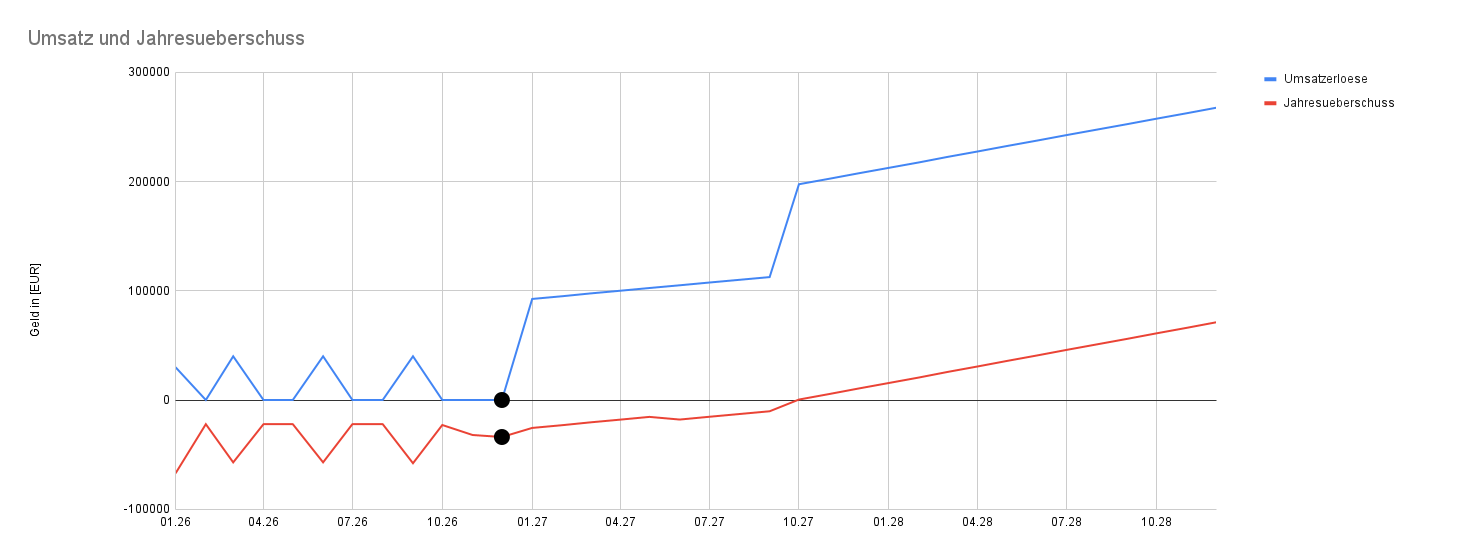
\includegraphics[width=15cm]{images/Umsatz und Jahresueberschuss.png}
    \caption{Umsatz und Jahres"uberschuss Planung}
    \label{fig:umsatzplanung}
\end{figure}

\subsection{Personalkosten}
Die detaillierte Personalplanung unseres Unternehmens, welche in \textbf{Abb. \ref{fig:personalplanung}} dargestellt ist, wurde strategisch an unsere Entwicklungs- und Markteintrittsphasen angepasst. Zunächst konzentriert sich der Personalausbau auf die Zeit vor dem Markteintritt. In dieser Phase werden zusätzlich zu den Kernentwicklern Mitarbeiter für den Vertrieb und den Einkauf eingestellt, um die Kommerzialisierung vorzubereiten. Aus Kostengründen und da die eigenständige Fertigung als unrentabel eingestuft wurde, werden keine Produktionsmitarbeiter eingestellt; die Hardware wird fertig bezogen.

Hinsichtlich der Vergütung ist eine Gehaltserhöhung von 500 € im Monat für jeden Mitarbeiter nach dem ersten Jahr vorgesehen. Die Personalnebenkosten steigen ebenfalls an, insbesondere durch die Aufnahme von Vertriebs- und Einkaufspersonal, da zusätzliche freiwillige Leistungen wie Tankkarten für die Vertriebsmitarbeiter geplant sind. Die drei Gründer verzichten im ersten Jahr aufgrund der angespannten wirtschaftlichen Lage vollständig auf ein Gehalt. Eine eigene Vergütung ist erst ab Beginn des zweiten Geschäftsjahres vorgesehen. Die Personalplanung sieht aufgrund der anfangs geringen Stückzahlen einen schlanken Personalstamm vor, der sich aus drei Fullstack-Entwicklern, zwei Data Engineers und einem Data Scientist zusammensetzt, was den klaren Fokus auf die Softwareentwicklung unterstreicht.

\begin{figure}[ht!]
    \centering
    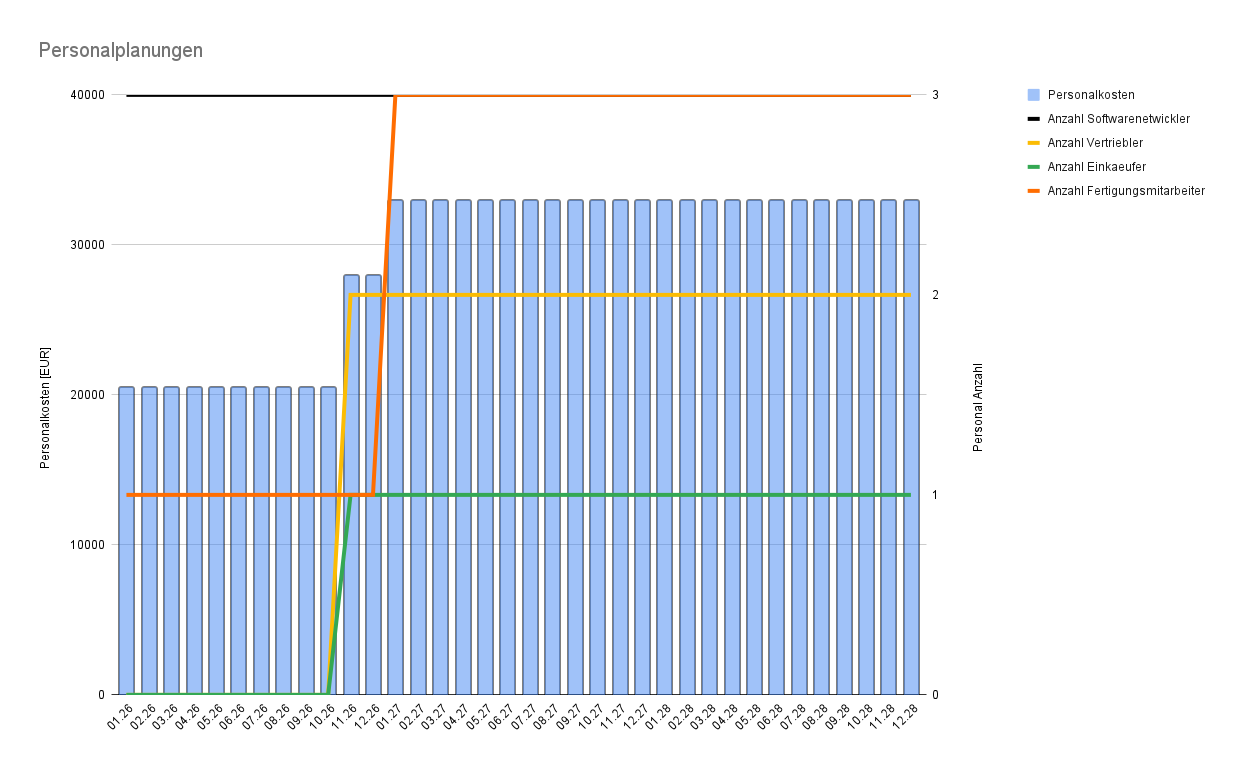
\includegraphics[width=15cm]{images/Personalplanungen.png}
    \caption{Personalplanung}
    \label{fig:personalplanung}
\end{figure}

\subsection{Cashflow Planungen}

\begin{figure}[ht!]
    \centering
    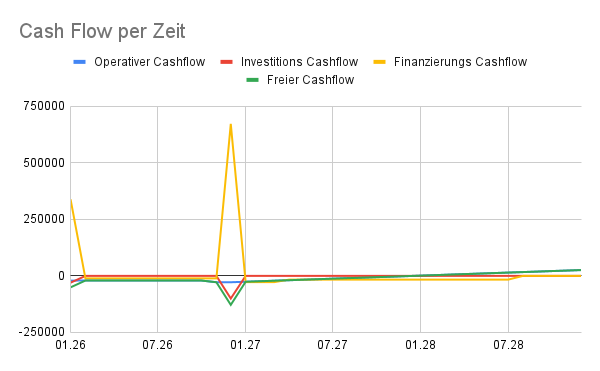
\includegraphics[width=15cm]{images/Cash Flow per Zeit.png}
    \caption{Cashflow Planung}
    \label{fig:cashflow_planung}
\end{figure}

Wie in \textbf{Abb. \ref{fig:cashflow_planung}} ersichtlich, ist der operative Cashflow in der Anfangsphase aufgrund der Personalkosten für die Entwickler negativ, da die Umsatzerlöse diese Kosten noch nicht decken. Im Einklang mit unserer Strategie, eine geringe Verschuldung zu priorisieren, wird der Investitions-Cashflow ausschließlich für gezielte Marketingaktivitäten und den Erwerb der Vertriebsfahrzeuge genutzt. Der operative Cashflow wird, synchron mit dem Jahresüberschuss, nach 22 Monaten erstmals in den positiven Bereich wechseln.

Unsere Finanzierungsstrategie ist zweistufig aufgebaut, um den Liquiditätsbedarf in jeder Unternehmensphase optimal zu decken. In der initialen Seed- und Startup-Phase ist es von entscheidender Bedeutung, die Kosten des ersten Jahres zu sichern. Da in dieser Phase noch keine Umsatzzahlen vorliegen, gehen wir davon aus, dass Bankkredite zu guten Konditionen nur schwer zu erhalten sind. Daher werden wir uns an Venture-Capital-Unternehmen und Business Angels wenden. Diese sollen uns 350.000 € als Eigenkapital im Austausch gegen Unternehmensanteile bereitstellen und uns gleichzeitig wichtige Kontakte zu potenziellen Pilotkunden vermitteln.

Sobald wir erste Erfolge, funktionierende Produkte und potenzielle Aufträge vorweisen können, werden wir bei einer Bank einen langfristigen Kredit in Höhe von 800.000 € beantragen. Dieser gestaffelte Ansatz ermöglicht es uns, die Kontrolle über das Startup zu behalten und die Entscheidungsprozesse schlank und agil zu gestalten.



\subsection{Profitabilit"at}
Um die Profatibilit"at zu errechen, wird eine mehrstufige Deckungsbeitragsrechnung durchgef"urt \textbf{Abb. \ref{fig:deckungsbeitrag_planung}}. Aufgrund der kleinen St"uckzahlen und der kleinen Unternehmensaufbaufs wird auf den Deckungsbeitrag 3 und 4 verzichtet.

Dabei ist erkenntlich dass die variablen Kosten immer gedeckt werden und der Deckungsbeitrag 2, indem die operativen Personalkosten (Vetrieb, Einkauf) auch bereits nach einem halben Jahr nach Markteintritt gedeckelt sein werden. 

\begin{figure}[ht!]
    \centering
    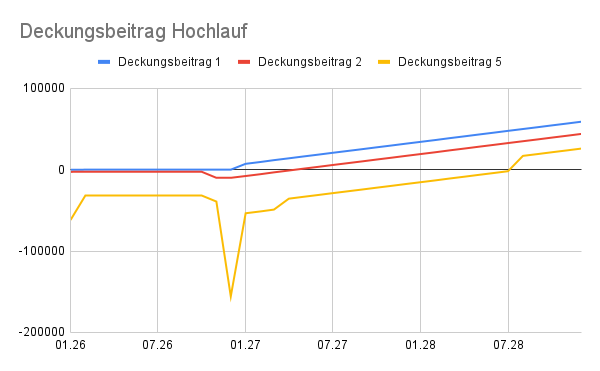
\includegraphics[width=15cm]{images/Deckungsbeitrag Hochlauf.png}
    \caption{Deckungsbeitrag Planung}
    \label{fig:deckungsbeitrag_planung}
\end{figure}





\begin{figure}[ht!]
    \centering
    % Subfigure für Q1 2027
    \begin{subfigure}[t]{0.45\textwidth}
        \centering
        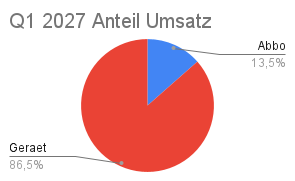
\includegraphics[width=\textwidth]{images/Q1 2027 Anteil Umsatz.png}
        \caption{Umsatzanteil Q1 2027}
        \label{fig:umsatzanteil2027q1}
    \end{subfigure}
    \hfill % Fügt horizontalen Abstand zwischen den Subfigures ein
    % Subfigure für Q4 2028
    \begin{subfigure}[t]{0.45\textwidth}
        \centering
        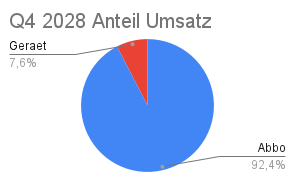
\includegraphics[width=\textwidth]{images/Q4 2028 Anteil Umsatz.png}
        \caption{Umsatzanteil Q4 2028}
        \label{fig:umsatzanteil2028q4}
    \end{subfigure}
    \caption{Vergleich der Umsatzanteile in Q1 2027 und Q4 2028}
    \label{fig:umsatzvergleich}
\end{figure}

Wie \textbf{Abb. \ref{fig:umsatzvergleich}} zeigt, wird der Verkauf der Ger"ate f"ur den Gesamtumsatz immer geringer und die Abonementpreise werden immer wichtiger f"ur den Umsatz. 


\subsection{Kapitalverlauf}
\label{cap:Kapitalverlauf}
Wie die Darstellung des Kapitalverlaufs in Abb. \ref{fig:kapitalverlauf} zeigt, wird der Kassenbestand zu keinem Zeitpunkt negativ sein. Die Kombination aus den aufgenommenen Krediten und den Eigenkapitalerhöhungen durch Investoren reicht aus, um die Seed- und Startup-Phase erfolgreich zu überstehen.

Sobald der operative Deckungsbeitrag erstmals positiv ist, kann das Unternehmen weitere Produktionsausweitungen und umfangreiche Marketinginvestitionen aus eigener Kraft finanzieren, da die laufenden Einnahmen ausreichen, um die Kosten zu decken und die Liquidität zu sichern.

\begin{figure}[ht!]
    \centering
    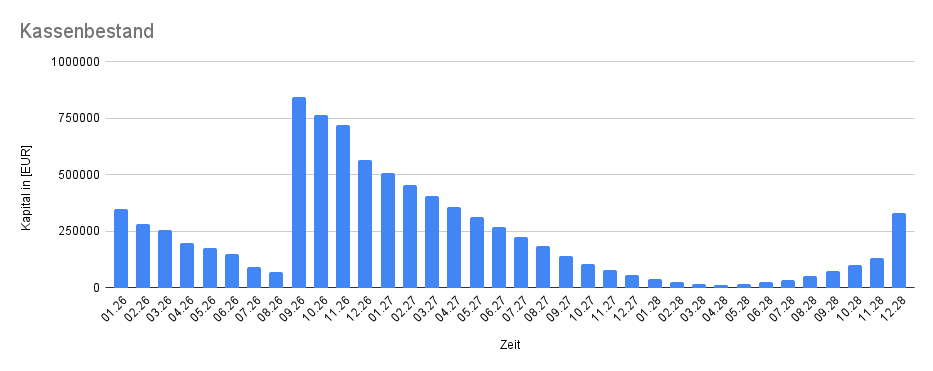
\includegraphics[width=15cm]{images/Kapital.png}
    \caption{Kapitalverlauf}
    \label{fig:kapitalverlauf}
\end{figure}

\newpage
\section{Anhang}


\begin{figure}[ht!]
    \centering
    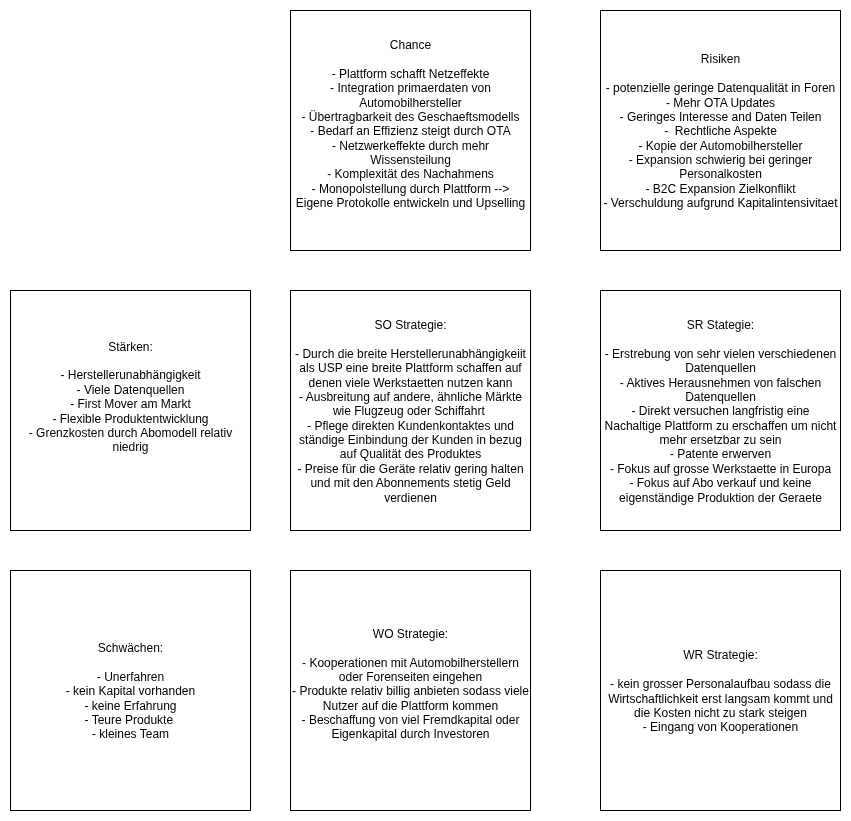
\includegraphics[width=15cm]{images/SWOT.png}
    \caption{SWOT Matrix}
\end{figure}


% Please add the following required packages to your document preamble:
% \usepackage[table,xcdraw]{xcolor}
% Beamer presentation requires \usepackage{colortbl} instead of \usepackage[table,xcdraw]{xcolor}
% Please add the following required packages to your document preamble:
% \usepackage[table,xcdraw]{xcolor}
% Beamer presentation requires \usepackage{colortbl} instead of \usepackage[table,xcdraw]{xcolor}
\begin{table}[]
\begin{tabular}{
>{\columncolor[HTML]{FFFFFF}}l 
>{\columncolor[HTML]{FFFFFF}}l 
>{\columncolor[HTML]{FFFFFF}}l }
{\color[HTML]{000000} } & {\color[HTML]{000000} \textbf{Total}} & {\color[HTML]{000000} \textbf{Geschäftsjahr 1}} \\
{\color[HTML]{000000} \textbf{AKTIVA}} & {\color[HTML]{000000} } & {\color[HTML]{000000} } \\
{\color[HTML]{000000} } & {\color[HTML]{000000} } & {\color[HTML]{000000} } \\
{\color[HTML]{000000} \textbf{A. Anlagevernögen}} & {\color[HTML]{000000} } & {\color[HTML]{000000} } \\
{\color[HTML]{000000} I. Immaterielle Vermögensgegenstände} & {\color[HTML]{000000} } & {\color[HTML]{000000} } \\
{\color[HTML]{000000} \textit{1. Entgelt erworbene Konzessionen, gewerbliche Schutzrechte}} & {\color[HTML]{000000} } & {\color[HTML]{000000} } \\
{\color[HTML]{000000} \textit{2. Geleistete Anzahlungen}} & {\color[HTML]{000000} } & {\color[HTML]{000000} 0,00€} \\
{\color[HTML]{000000} \textit{3. Andere}} & {\color[HTML]{000000} } & {\color[HTML]{000000} } \\
{\color[HTML]{000000} II. Sachanlagen} & {\color[HTML]{000000} } & {\color[HTML]{000000} } \\
{\color[HTML]{000000} \textit{1. Grundstücke, grundstücksgleiche Rechte und Bauten}} & {\color[HTML]{000000} } & {\color[HTML]{000000} } \\
{\color[HTML]{000000} \textit{2. Andere Anlagen, Betriebs- und Geschäftsausstattung}} & {\color[HTML]{000000} } & {\color[HTML]{000000} } \\
{\color[HTML]{000000} \textit{3. Geleistete Anzahlungen und Anlagen im Bau}} & {\color[HTML]{000000} } & {\color[HTML]{000000} } \\
{\color[HTML]{000000} \textit{4. Andere}} & {\color[HTML]{000000} } & {\color[HTML]{000000} 98,61€} \\
{\color[HTML]{000000} III. Finanzanlagen} & {\color[HTML]{000000} } & {\color[HTML]{000000} } \\
{\color[HTML]{000000} \textit{1. Anteile an verbundenen Unternehmen}} & {\color[HTML]{000000} } & {\color[HTML]{000000} } \\
{\color[HTML]{000000} \textit{2. Andere}} & {\color[HTML]{000000} } & {\color[HTML]{000000} } \\
{\color[HTML]{000000} \textbf{Total A}} & {\color[HTML]{000000} } & {\color[HTML]{000000} } \\
{\color[HTML]{000000} } & {\color[HTML]{000000} } & {\color[HTML]{000000} } \\
{\color[HTML]{000000} \textbf{B. Umlaufvermögen}} & {\color[HTML]{000000} } & {\color[HTML]{000000} } \\
{\color[HTML]{000000} I. Vorräte} & {\color[HTML]{000000} } & {\color[HTML]{000000} } \\
{\color[HTML]{000000} \textit{1. Roh-. Hilfs- und Betriebsstoffe}} & {\color[HTML]{000000} } & {\color[HTML]{000000} 0,00€} \\
{\color[HTML]{000000} \textit{2. Unfertige Leistungen}} & {\color[HTML]{000000} } & {\color[HTML]{000000} 0,00€} \\
{\color[HTML]{000000} \textit{3. Waren}} & {\color[HTML]{000000} } & {\color[HTML]{000000} 0,00€} \\
{\color[HTML]{000000} II. Forderungen und sonstige Vermögensgegenstände} & {\color[HTML]{000000} } & {\color[HTML]{000000} } \\
{\color[HTML]{000000} \textit{1. Forderungen aus Lieferungen und Leistungen}} & {\color[HTML]{000000} } & {\color[HTML]{000000} 0,00€} \\
{\color[HTML]{000000} \textit{2. Forderungen gegen verbundene Unternehmen}} & {\color[HTML]{000000} } & {\color[HTML]{000000} 0,00€} \\
{\color[HTML]{000000} \textit{3. Sonstige Vermögensgegenstände}} & {\color[HTML]{000000} } & {\color[HTML]{000000} 0,00€} \\
{\color[HTML]{000000} III. Wertpapiere} & {\color[HTML]{000000} } & {\color[HTML]{000000} 0,00€} \\
{\color[HTML]{000000} IV. Kassenbestand} & {\color[HTML]{000000} } & {\color[HTML]{000000} 431,00€} \\
{\color[HTML]{000000} \textbf{Total B}} & {\color[HTML]{000000} } & {\color[HTML]{000000} \textbf{0,00€}} \\
{\color[HTML]{000000} } & {\color[HTML]{000000} } & {\color[HTML]{000000} } \\
{\color[HTML]{000000} \textbf{C. Rechnungsabgrenzungsposten}} & {\color[HTML]{000000} } & {\color[HTML]{000000} \textbf{0,00€}} \\
{\color[HTML]{000000} \textbf{D. Aktive latente Steuern}} & {\color[HTML]{000000} } & {\color[HTML]{000000} \textbf{0,00€}} \\
{\color[HTML]{000000} \textbf{E. Aktiver Unterschiedsbetrag aus der Vermögensverrechnung}} & {\color[HTML]{000000} } & {\color[HTML]{000000} \textbf{0,00€}} \\
{\color[HTML]{000000} } & {\color[HTML]{000000} } & {\color[HTML]{000000} } \\
{\color[HTML]{000000} \textbf{Gesamtsumme}} & {\color[HTML]{000000} } & {\color[HTML]{000000} \textbf{529,61€}}
\end{tabular}
\caption{Aktiva Bilanz nach 1. Jahr}
\end{table}

\newpage

% Please add the following required packages to your document preamble:
% \usepackage[table,xcdraw]{xcolor}
% Beamer presentation requires \usepackage{colortbl} instead of \usepackage[table,xcdraw]{xcolor}
\begin{table}[]
\begin{tabular}{
>{\columncolor[HTML]{FFFFFF}}l 
>{\columncolor[HTML]{FFFFFF}}l 
>{\columncolor[HTML]{FFFFFF}}l }
{\color[HTML]{000000} } & {\color[HTML]{000000} \textbf{Total}} & {\color[HTML]{000000} \textbf{Geschäftsjahr 1}} \\
{\color[HTML]{000000} \textbf{AKTIVA}} & {\color[HTML]{000000} } & {\color[HTML]{000000} } \\
{\color[HTML]{000000} } & {\color[HTML]{000000} } & {\color[HTML]{000000} } \\
{\color[HTML]{000000} \textbf{PASSIVA}} & {\color[HTML]{000000} \textbf{J1}} & {\color[HTML]{000000} } \\
{\color[HTML]{000000} } & {\color[HTML]{000000} } & {\color[HTML]{000000} } \\
{\color[HTML]{000000} \textit{\textbf{A. EIGENKAPITAL}}} & {\color[HTML]{000000} } & {\color[HTML]{000000} } \\
{\color[HTML]{000000} \textit{I. Gezeichnetes Kapital}} & {\color[HTML]{000000} -270,39€} & {\color[HTML]{000000} 0,00€} \\
{\color[HTML]{000000} \textit{II. Kapitalrücklagen}} & {\color[HTML]{000000} 0,00€} & {\color[HTML]{000000} } \\
{\color[HTML]{000000} III. Gewinrücklagen} & {\color[HTML]{000000} 0,00€} & {\color[HTML]{000000} } \\
{\color[HTML]{000000} \textit{IV. Gewinnvortrag/ Verlustvortrag}} & {\color[HTML]{000000} 0,00€} & {\color[HTML]{000000} } \\
{\color[HTML]{000000} \textit{V. Jahresüberschuss/ Jahresfehlbetrag}} & {\color[HTML]{000000} 0,00€} & {\color[HTML]{000000} } \\
{\color[HTML]{000000} \textit{}} & {\color[HTML]{000000} } & {\color[HTML]{000000} } \\
{\color[HTML]{000000} \textit{}} & {\color[HTML]{000000} } & {\color[HTML]{000000} 98,61€} \\
{\color[HTML]{000000} \textbf{Total A.}} & {\color[HTML]{000000} \textbf{0}} & {\color[HTML]{000000} } \\
{\color[HTML]{000000} \textit{}} & {\color[HTML]{000000} } & {\color[HTML]{000000} } \\
{\color[HTML]{000000} \textit{\textbf{B. Rückstellungen}}} & {\color[HTML]{000000} } & {\color[HTML]{000000} } \\
{\color[HTML]{000000} \textbf{1. Rückstellungen für Pensionen und ähnliche Verpflichtungen}} & {\color[HTML]{000000} 0,00€} & {\color[HTML]{000000} } \\
{\color[HTML]{000000} 2. Steuerrückstellungen} & {\color[HTML]{000000} 0,00€} & {\color[HTML]{000000} } \\
{\color[HTML]{000000} \textbf{3. Sonstige Rückstellungen}} & {\color[HTML]{000000} 0,00€} & {\color[HTML]{000000} } \\
{\color[HTML]{000000} \textbf{Total B.}} & {\color[HTML]{000000} 0,00€} & {\color[HTML]{000000} } \\
{\color[HTML]{000000} \textit{}} & {\color[HTML]{000000} } & {\color[HTML]{000000} 0,00€} \\
{\color[HTML]{000000} \textit{\textbf{C. Verbindlichkeiten}}} & {\color[HTML]{000000} } & {\color[HTML]{000000} 0,00€} \\
{\color[HTML]{000000} \textit{1. Verbindlichkeiten gegenüber Kreditinstituten}} & {\color[HTML]{000000} 800,00€} & {\color[HTML]{000000} 0,00€} \\
{\color[HTML]{000000} 2. Verbindlichkeiten aus Lieferungen und Leistungen} & {\color[HTML]{000000} 0,00€} & {\color[HTML]{000000} } \\
{\color[HTML]{000000} \textit{3. Verbindlichkeiten gegenüber verbundenen Unternehmen}} & {\color[HTML]{000000} 0,00€} & {\color[HTML]{000000} 0,00€} \\
{\color[HTML]{000000} \textit{4. Verbindlichkeiten}} & {\color[HTML]{000000} 0,00€} & {\color[HTML]{000000} 0,00€} \\
{\color[HTML]{000000} \textit{\textbf{Total C.}}} & {\color[HTML]{000000} 0,00€} & {\color[HTML]{000000} 0,00€} \\
{\color[HTML]{000000} } & {\color[HTML]{000000} } & {\color[HTML]{000000} 0,00€} \\
{\color[HTML]{000000} \textbf{D. Rechnungsabgrenzungsposten}} & {\color[HTML]{000000} \textbf{0}} & {\color[HTML]{000000} 431,00€} \\
{\color[HTML]{000000} \textbf{E. Passive latente Steuern}} & {\color[HTML]{000000} \textbf{0}} & {\color[HTML]{000000} \textbf{0,00€}} \\
{\color[HTML]{000000} } & {\color[HTML]{000000} } & {\color[HTML]{000000} } \\
{\color[HTML]{000000} \textbf{}} & {\color[HTML]{000000} } & {\color[HTML]{000000} \textbf{0,00€}} \\
{\color[HTML]{000000} \textbf{}} & {\color[HTML]{000000} } & {\color[HTML]{000000} \textbf{0,00€}} \\
{\color[HTML]{000000} \textbf{Gesamtsumme (A+B+C+D+E)}} & {\color[HTML]{000000} \textbf{529,61€}} & {\color[HTML]{000000} \textbf{0,00€}}
\end{tabular}
\caption{Passiva Bilanz nach 1. Jahr}
\end{table}



% \begin{landscape}
% \begin{table}[]
% \begin{tabular}{lrrrrrrrrrrrrrrrrrrrrrrrrrrrrrrrrrrrr}
% \cellcolor[HTML]{FFFFFF}{\color[HTML]{000000} \textbf{}} & \cellcolor[HTML]{FFFFFF}{\color[HTML]{000000} 01.26} & \cellcolor[HTML]{FFFFFF}{\color[HTML]{000000} 02.26} & {\color[HTML]{000000} 03.26} & {\color[HTML]{000000} 04.26} & {\color[HTML]{000000} 05.26} & {\color[HTML]{000000} 06.26} & {\color[HTML]{000000} 07.26} & {\color[HTML]{000000} 08.26} & {\color[HTML]{000000} 09.26} & {\color[HTML]{000000} 10.26} & {\color[HTML]{000000} 11.26} & {\color[HTML]{000000} 12.26} & {\color[HTML]{000000} 01.27} & {\color[HTML]{000000} 02.27} & {\color[HTML]{000000} 03.27} & {\color[HTML]{000000} 04.27} & {\color[HTML]{000000} 05.27} & {\color[HTML]{000000} 06.27} & {\color[HTML]{000000} 07.27} & {\color[HTML]{000000} 08.27} & {\color[HTML]{000000} 09.27} & {\color[HTML]{000000} 10.27} & {\color[HTML]{000000} 11.27} & {\color[HTML]{000000} 12.27} & {\color[HTML]{000000} 01.28} & {\color[HTML]{000000} 02.28} & {\color[HTML]{000000} 03.28} & {\color[HTML]{000000} 04.28} & {\color[HTML]{000000} 05.28} & {\color[HTML]{000000} 06.28} & {\color[HTML]{000000} 07.28} & {\color[HTML]{000000} 08.28} & {\color[HTML]{000000} 09.28} & {\color[HTML]{000000} 10.28} & {\color[HTML]{000000} 11.28} & {\color[HTML]{000000} 12.28} \\
% \cellcolor[HTML]{FFFFFF}{\color[HTML]{000000} Neue Geraete 22K unabh. werkstaette} & \cellcolor[HTML]{FFFFFF}{\color[HTML]{000000} 10} & \cellcolor[HTML]{FFFFFF}{\color[HTML]{000000} 0} & {\color[HTML]{000000} 10} & {\color[HTML]{000000} 0} & {\color[HTML]{000000} 0} & {\color[HTML]{000000} 10} & {\color[HTML]{000000} 0} & {\color[HTML]{000000} 0} & {\color[HTML]{000000} 10} & {\color[HTML]{000000} 0} & {\color[HTML]{000000} 0} & {\color[HTML]{000000} 0} & {\color[HTML]{000000} 10} & {\color[HTML]{000000} 10} & {\color[HTML]{000000} 10} & {\color[HTML]{000000} 10} & {\color[HTML]{000000} 10} & {\color[HTML]{000000} 10} & {\color[HTML]{000000} 10} & {\color[HTML]{000000} 10} & {\color[HTML]{000000} 10} & {\color[HTML]{000000} 20} & {\color[HTML]{000000} 20} & {\color[HTML]{000000} 20} & {\color[HTML]{000000} 20} & {\color[HTML]{000000} 20} & {\color[HTML]{000000} 20} & {\color[HTML]{000000} 20} & {\color[HTML]{000000} 20} & {\color[HTML]{000000} 20} & {\color[HTML]{000000} 20} & {\color[HTML]{000000} 20} & {\color[HTML]{000000} 20} & {\color[HTML]{000000} 20} & {\color[HTML]{000000} 20} & {\color[HTML]{000000} 20} \\
% \cellcolor[HTML]{FFFFFF}{\color[HTML]{000000} Preis Neues Geraet} & \cellcolor[HTML]{FFFFFF}{\color[HTML]{000000} 3000} & \cellcolor[HTML]{FFFFFF}{\color[HTML]{000000} 0} & {\color[HTML]{000000} 4000} & {\color[HTML]{000000} 0} & {\color[HTML]{000000} 0} & {\color[HTML]{000000} 4000} & {\color[HTML]{000000} 0} & {\color[HTML]{000000} 0} & {\color[HTML]{000000} 4000} & {\color[HTML]{000000} 0} & {\color[HTML]{000000} 0} & {\color[HTML]{000000} 0} & {\color[HTML]{000000} 8000} & {\color[HTML]{000000} 8000} & {\color[HTML]{000000} 8000} & {\color[HTML]{000000} 8000} & {\color[HTML]{000000} 8000} & {\color[HTML]{000000} 8000} & {\color[HTML]{000000} 8000} & {\color[HTML]{000000} 8000} & {\color[HTML]{000000} 8000} & {\color[HTML]{000000} 8000} & {\color[HTML]{000000} 8000} & {\color[HTML]{000000} 8000} & {\color[HTML]{000000} 8000} & {\color[HTML]{000000} 8000} & {\color[HTML]{000000} 8000} & {\color[HTML]{000000} 8000} & {\color[HTML]{000000} 8000} & {\color[HTML]{000000} 8000} & {\color[HTML]{000000} 8000} & {\color[HTML]{000000} 8000} & {\color[HTML]{000000} 8000} & {\color[HTML]{000000} 8000} & {\color[HTML]{000000} 8000} & {\color[HTML]{000000} 8000} \\
% \cellcolor[HTML]{FFFFFF}{\color[HTML]{000000} Aktive Geraete} & \cellcolor[HTML]{FFFFFF}{\color[HTML]{000000} 10} & \cellcolor[HTML]{FFFFFF}{\color[HTML]{000000} 10} & {\color[HTML]{000000} 20} & {\color[HTML]{000000} 20} & {\color[HTML]{000000} 20} & {\color[HTML]{000000} 30} & {\color[HTML]{000000} 30} & {\color[HTML]{000000} 30} & {\color[HTML]{000000} 40} & {\color[HTML]{000000} 40} & {\color[HTML]{000000} 40} & {\color[HTML]{000000} 40} & {\color[HTML]{000000} 50} & {\color[HTML]{000000} 60} & {\color[HTML]{000000} 70} & {\color[HTML]{000000} 80} & {\color[HTML]{000000} 90} & {\color[HTML]{000000} 100} & {\color[HTML]{000000} 110} & {\color[HTML]{000000} 120} & {\color[HTML]{000000} 130} & {\color[HTML]{000000} 150} & {\color[HTML]{000000} 170} & {\color[HTML]{000000} 190} & {\color[HTML]{000000} 210} & {\color[HTML]{000000} 230} & {\color[HTML]{000000} 250} & {\color[HTML]{000000} 270} & {\color[HTML]{000000} 290} & {\color[HTML]{000000} 310} & {\color[HTML]{000000} 330} & {\color[HTML]{000000} 350} & {\color[HTML]{000000} 370} & {\color[HTML]{000000} 390} & {\color[HTML]{000000} 410} & {\color[HTML]{000000} 430} \\
% \cellcolor[HTML]{FFFFFF}{\color[HTML]{000000} \textit{Abo Preis}} & \cellcolor[HTML]{FFFFFF}{\color[HTML]{000000} 0} & \cellcolor[HTML]{FFFFFF}{\color[HTML]{000000} 0} & {\color[HTML]{000000} 0} & {\color[HTML]{000000} 0} & {\color[HTML]{000000} 0} & {\color[HTML]{000000} 0} & {\color[HTML]{000000} 0} & {\color[HTML]{000000} 0} & {\color[HTML]{000000} 0} & {\color[HTML]{000000} 0} & {\color[HTML]{000000} 0} & {\color[HTML]{000000} 0} & {\color[HTML]{000000} 250} & {\color[HTML]{000000} 250} & {\color[HTML]{000000} 250} & {\color[HTML]{000000} 250} & {\color[HTML]{000000} 250} & {\color[HTML]{000000} 250} & {\color[HTML]{000000} 250} & {\color[HTML]{000000} 250} & {\color[HTML]{000000} 250} & {\color[HTML]{000000} 250} & {\color[HTML]{000000} 250} & {\color[HTML]{000000} 250} & {\color[HTML]{000000} 250} & {\color[HTML]{000000} 250} & {\color[HTML]{000000} 250} & {\color[HTML]{000000} 250} & {\color[HTML]{000000} 250} & {\color[HTML]{000000} 250} & {\color[HTML]{000000} 250} & {\color[HTML]{000000} 250} & {\color[HTML]{000000} 250} & {\color[HTML]{000000} 250} & {\color[HTML]{000000} 250} & {\color[HTML]{000000} 250} \\
% \rowcolor[HTML]{B6D7A8} 
% {\color[HTML]{000000} UE aus verkauften Waren \& DL} & {\color[HTML]{000000} 30000} & {\color[HTML]{000000} 0} & {\color[HTML]{000000} 40000} & {\color[HTML]{000000} 0} & {\color[HTML]{000000} 0} & {\color[HTML]{000000} 40000} & {\color[HTML]{000000} 0} & {\color[HTML]{000000} 0} & {\color[HTML]{000000} 40000} & {\color[HTML]{000000} 0} & {\color[HTML]{000000} 0} & {\color[HTML]{000000} 0} & {\color[HTML]{000000} 92500} & {\color[HTML]{000000} 95000} & {\color[HTML]{000000} 97500} & {\color[HTML]{000000} 100000} & {\color[HTML]{000000} 102500} & {\color[HTML]{000000} 105000} & {\color[HTML]{000000} 107500} & {\color[HTML]{000000} 110000} & {\color[HTML]{000000} 112500} & {\color[HTML]{000000} 197500} & {\color[HTML]{000000} 202500} & {\color[HTML]{000000} 207500} & {\color[HTML]{000000} 212500} & {\color[HTML]{000000} 217500} & {\color[HTML]{000000} 222500} & {\color[HTML]{000000} 227500} & {\color[HTML]{000000} 232500} & {\color[HTML]{000000} 237500} & {\color[HTML]{000000} 242500} & {\color[HTML]{000000} 247500} & {\color[HTML]{000000} 252500} & {\color[HTML]{000000} 257500} & {\color[HTML]{000000} 262500} & {\color[HTML]{000000} 267500}
% \end{tabular}
% \end{table}
% \end{landscape}

\begin{sidewaystable}[h!]
    \centering
    \caption{Tabelle 1/3: Ertragsdaten (Jan 26 - Dez 26)}
    \begin{tabular}{|l|*{12}{c|}}
        \hline
        \rowcolor[HTML]{EFEFEF}
        \textbf{Kennzahlen} & \textbf{01.26} & \textbf{02.26} & \textbf{03.26} & \textbf{04.26} & \textbf{05.26} & \textbf{06.26} & \textbf{07.26} & \textbf{08.26} & \textbf{09.26} & \textbf{10.26} & \textbf{11.26} & \textbf{12.26} \\
        \hline
        Neue Geraete 22K unabh. werkstaette & 10 & 0 & 10 & 0 & 0 & 10 & 0 & 0 & 10 & 0 & 0 & 0 \\
        Preis Neues Geraet & 3000 & 0 & 4000 & 0 & 0 & 4000 & 0 & 0 & 4000 & 0 & 0 & 0 \\
        Aktive Geraete & 10 & 10 & 20 & 20 & 20 & 30 & 30 & 30 & 40 & 40 & 40 & 40 \\
        \textit{Abo Preis} & 0 & 0 & 0 & 0 & 0 & 0 & 0 & 0 & 0 & 0 & 0 & 0 \\
        \rowcolor[HTML]{B6D7A8} 
        UE aus verkauften Waren \& DL & 30000 & 0 & 40000 & 0 & 0 & 40000 & 0 & 0 & 40000 & 0 & 0 & 0 \\
        \hline
    \end{tabular}
\end{sidewaystable}

\begin{sidewaystable}[h!]
    \centering
    \caption{Tabelle 2/3: Ertragsdaten (Jan 27 - Dez 27)}
    \begin{tabular}{|l|*{12}{c|}}
        \hline
        \rowcolor[HTML]{EFEFEF}
        \textbf{Kennzahlen} & \textbf{01.27} & \textbf{02.27} & \textbf{03.27} & \textbf{04.27} & \textbf{05.27} & \textbf{06.27} & \textbf{07.27} & \textbf{08.27} & \textbf{09.27} & \textbf{10.27} & \textbf{11.27} & \textbf{12.27} \\
        \hline
        Neue Geraete 22K unabh. werkstaette & 10 & 10 & 10 & 10 & 10 & 10 & 10 & 10 & 10 & 20 & 20 & 20 \\
        Preis Neues Geraet & 8000 & 8000 & 8000 & 8000 & 8000 & 8000 & 8000 & 8000 & 8000 & 8000 & 8000 & 8000 \\
        Aktive Geraete & 50 & 60 & 70 & 80 & 90 & 100 & 110 & 120 & 130 & 150 & 170 & 190 \\
        \textit{Abo Preis} & 250 & 250 & 250 & 250 & 250 & 250 & 250 & 250 & 250 & 250 & 250 & 250 \\
        \rowcolor[HTML]{B6D7A8} 
        UE aus verkauften Waren \& DL & 92500 & 95000 & 97500 & 100000 & 102500 & 105000 & 107500 & 110000 & 112500 & 197500 & 202500 & 207500 \\
        \hline
    \end{tabular}
\end{sidewaystable}

\begin{sidewaystable}[h!]
    \centering
    \caption{Tabelle 3/3: Ertragsdaten (Jan 28 - Dez 28)}
    \begin{tabular}{|l|*{12}{c|}}
        \hline
        \rowcolor[HTML]{EFEFEF}
        \textbf{Kennzahlen} & \textbf{01.28} & \textbf{02.28} & \textbf{03.28} & \textbf{04.28} & \textbf{05.28} & \textbf{06.28} & \textbf{07.28} & \textbf{08.28} & \textbf{09.28} & \textbf{10.28} & \textbf{11.28} & \textbf{12.28} \\
        \hline
        Neue Geraete 22K unabh. werkstaette & 20 & 20 & 20 & 20 & 20 & 20 & 20 & 20 & 20 & 20 & 20 & 20 \\
        Preis Neues Geraet & 8000 & 8000 & 8000 & 8000 & 8000 & 8000 & 8000 & 8000 & 8000 & 8000 & 8000 & 8000 \\
        Aktive Geraete & 210 & 230 & 250 & 270 & 290 & 310 & 330 & 350 & 370 & 390 & 410 & 430 \\
        \textit{Abo Preis} & 250 & 250 & 250 & 250 & 250 & 250 & 250 & 250 & 250 & 250 & 250 & 250 \\
        \rowcolor[HTML]{B6D7A8} 
        UE aus verkauften Waren \& DL & 212500 & 217500 & 222500 & 227500 & 232500 & 237500 & 242500 & 247500 & 252500 & 257500 & 262500 & 267500 \\
        \hline
    \end{tabular}
\end{sidewaystable}



% \begin{sidewaystable}[h!]
%     \centering
%     \caption{Kostenplanung (Jan 28 - Dez 28)}
%     \label{tab:kostenplanung3}
%     \begin{tabularx}{\linewidth}{|l|*{12}{>{\centering\arraybackslash}X|}}
%         \hline
%         \rowcolor[HTML]{EFEFEF}
%         \textbf{Kostenart} & \textbf{01.28} & \textbf{02.28} & \textbf{03.28} & \textbf{04.28} & \textbf{05.28} & \textbf{06.28} & \textbf{07.28} & \textbf{08.28} & \textbf{09.28} & \textbf{10.28} & \textbf{11.28} & \textbf{12.28} \\
%         \hline
%         Personalkosten & 54830 & 54830 & 54830 & 54830 & 54830 & 54830 & 54830 & 54830 & 54830 & 54830 & 54830 & 54830 \\
%         Materialkosten pro Geraet & 7000 & 7000 & 7000 & 7000 & 7000 & 7000 & 7000 & 7000 & 7000 & 7000 & 7000 & 7000 \\
%         Materialkosten & 140000 & 140000 & 140000 & 140000 & 140000 & 140000 & 140000 & 140000 & 140000 & 140000 & 140000 & 140000 \\
%         GPU Stunden & 770 & 843,33 & 916,67 & 990 & 1063,33 & 1136,67 & 1210 & 1283,33 & 1356,67 & 1430 & 1503,33 & 1576,67 \\
%         L4 GPU Kosten 70ct / h & 539 & 590,33 & 641,67 & 693 & 744,33 & 795,67 & 847 & 898,33 & 949,67 & 1001 & 1052,33 & 1103,67 \\
%         Webseite Hosting & 3 & 3 & 3 & 3 & 3 & 3 & 3 & 3 & 3 & 3 & 3 & 3 \\
%         kalkulierte Cloud Speicherkosten & 35 & 35 & 35 & 35 & 35 & 35 & 35 & 35 & 35 & 35 & 35 & 35 \\
%         Trainingzeiten & 18 & 18 & 18 & 18 & 18 & 18 & 18 & 18 & 18 & 18 & 18 & 18 \\
%         Trainingskosten 32,77 EUR h A100 AWS & 588,6 & 588,6 & 588,6 & 588,6 & 588,6 & 588,6 & 588,6 & 588,6 & 588,6 & 588,6 & 588,6 & 588,6 \\
%         Cloud Kosten & 1165,6 & 1216,93 & 1268,27 & 1319,6 & 1370,93 & 1422,27 & 1473,6 & 1524,93 & 1576,27 & 1627,6 & 1678,93 & 1730,27 \\
%         Miete & 1050 & 1050 & 1050 & 1050 & 1050 & 1050 & 1050 & 1050 & 1050 & 1050 & 1050 & 1050 \\
%         Marketing-investitionen Messe & 6000 & 6000 & 6000 & 6000 & 6000 & 6000 & 6000 & 6000 & 6000 & 6000 & 6000 & 6000 \\
%         Investitionen & 0 & 0 & 0 & 0 & 0 & 0 & 0 & 0 & 0 & 0 & 0 & 0 \\
%         Zinskosten & 700 & 700 & 700 & 700 & 700 & 700 & 700 & 700 & 700 & 700 & 700 & 700 \\
%         Tilgung & 20000 & 20000 & 20000 & 20000 & 20000 & 20000 & 20000 & 20000 & 20000 & 20000 & 20000 & 20000 \\
%         Abschreibungen & 1388,9 & 1388,9 & 1388,9 & 1388,9 & 1388,9 & 1388,9 & 1388,9 & 1388,9 & 1388,9 & 1388,9 & 1388,9 & 1388,9 \\
%         Rueckstellungen & & & & & & & & & & & & \\
%         Gesamt-aufwendungen & 225169,5 & 225220,83 & 225272,17 & 225323,5 & 225374,83 & 225426,17 & 225477,5 & 225528,83 & 225580,17 & 225631,5 & 225682,83 & 225734,17 \\
%         \hline
%     \end{tabularx}
% \end{sidewaystable}


\begin{sidewaystable}[h!]
    \centering
    \caption{Kostenplanung (Jan 26 - Dez 26)}
    \label{tab:kostenplanung1}
    \begin{tabularx}{\linewidth}{|p{3.5cm}|*{12}{>{\centering\arraybackslash}X|}}
        \hline
        \rowcolor[HTML]{EFEFEF}
        \textbf{Kostenart} & \textbf{01.26} & \textbf{02.26} & \textbf{03.26} & \textbf{04.26} & \textbf{05.26} & \textbf{06.26} & \textbf{07.26} & \textbf{08.26} & \textbf{09.26} & \textbf{10.26} & \textbf{11.26} & \textbf{12.26} \\
        \hline
        Personalkosten & 21960 & 21960 & 21960 & 21960 & 21960 & 21960 & 21960 & 21960 & 21960 & 21960 & 31110 & 31560 \\ \hline
        Materialkosten pro Geraet & 7500 & 7500 & 7500 & 7500 & 7500 & 7500 & 7500 & 7500 & 7500 & 7500 & 7500 & 7500 \\ \hline
        Materialkosten & 75000 & 0 & 75000 & 0 & 0 & 75000 & 0 & 0 & 75000 & 0 & 0 & 0 \\ \hline
        GPU Stunden & 36,67 & 36,67 & 73,33 & 73,33 & 73,33 & 110 & 110 & 110 & 146,67 & 146,67 & 146,67 & 146,67 \\ \hline
        L4 GPU Kosten 70ct / h & 25,67 & 25,67 & 51,33 & 51,33 & 51,33 & 77 & 77 & 77 & 102,67 & 102,67 & 102,67 & 102,67 \\ \hline
        Webseite Hosting & 3 & 3 & 3 & 3 & 3 & 3 & 3 & 3 & 3 & 3 & 3 & 3 \\ \hline
        kalkulierte Cloud Speicherkosten & 30 & 30 & 30 & 30 & 30 & 30 & 30 & 30 & 30 & 30 & 30 & 30 \\ \hline
        Trainingzeiten & 25 & 25 & 25 & 25 & 25 & 25 & 25 & 25 & 25 & 25 & 25 & 25 \\ \hline
        Trainingskosten 32,77 EUR h A100 AWS & 817,5 & 817,5 & 817,5 & 817,5 & 817,5 & 817,5 & 817,5 & 817,5 & 817,5 & 817,5 & 817,5 & 817,5 \\ \hline
        Cloud Kosten & 876,17 & 876,17 & 901,83 & 901,83 & 901,83 & 927,5 & 927,5 & 927,5 & 953,17 & 953,17 & 953,17 & 953,17 \\ \hline
        Miete & 1050 & 1050 & 1050 & 1050 & 1050 & 1050 & 1050 & 1050 & 1050 & 1050 & 1050 & 1050 \\ \hline
        Marketing-investitionen Messe & & & & & & & & & & & & 0 \\ \hline
        Investitionen & 0 & 0 & 0 & 0 & 0 & 0 & 0 & 0 & 0 & 0 & 100000 & 0 \\ \hline
        Zinskosten & 0 & 0 & 0 & 0 & 0 & 0 & 0 & 0 & 700 & 700 & 700 & 700 \\ \hline
        Tilgung & & & & & & & & & 20000 & 20000 & 20000 & 20000 \\ \hline
        Abschreibungen & & & & & & & & & & & & 1388,9 \\ \hline
        Rueckstellungen & & & & & & & & & & & & \\ \hline
        Gesamt-aufwendungen & 98916,17 & 23916,17 & 98941,83 & 23941,83 & 23941,83 & 98967,5 & 23967,5 & 23967,5 & 119693,17 & 44693,17 & 153843,17 & 55682,07 \\ 
        \hline
    \end{tabularx}
\end{sidewaystable}


\begin{sidewaystable}[h!]
    \centering
    \caption{Kostenplanung (Jan 27 - Dez 27)}
    \label{tab:kostenplanung2}
    \begin{tabularx}{\linewidth}{|p{2.5cm}|*{12}{>{\centering\arraybackslash}X|}}
        \hline
        \rowcolor[HTML]{EFEFEF}
        \textbf{Kostenart} & \textbf{01.27} & \textbf{02.27} & \textbf{03.27} & \textbf{04.27} & \textbf{05.27} & \textbf{06.27} & \textbf{07.27} & \textbf{08.27} & \textbf{09.27} & \textbf{10.27} & \textbf{11.27} & \textbf{12.27} \\
        \hline
        Personalkosten & 42540 & 42540 & 42540 & 42540 & 42540 & 47510 & 47510 & 47510 & 47510 & 54830 & 54830 & 54830 \\ \hline
        Materialkosten pro Geraet & 7300 & 7300 & 7300 & 7300 & 7300 & 7300 & 7300 & 7300 & 7300 & 7000 & 7000 & 7000 \\ \hline
        Materialkosten & 73000 & 73000 & 73000 & 73000 & 73000 & 73000 & 73000 & 73000 & 73000 & 140000 & 140000 & 140000 \\ \hline
        GPU Stunden & 183,33 & 220 & 256,67 & 293,33 & 330 & 366,67 & 403,33 & 440 & 476,67 & 550 & 623,33 & 696,67 \\ \hline
        L4 GPU Kosten 70ct / h & 128,33 & 154 & 179,67 & 205,33 & 231 & 256,67 & 282,33 & 308 & 333,67 & 385 & 436,33 & 487,67 \\ \hline
        Webseite Hosting & 3 & 3 & 3 & 3 & 3 & 3 & 3 & 3 & 3 & 3 & 3 & 3 \\ \hline
        kalkulierte Cloud Speicherkosten & 30 & 30 & 30 & 30 & 30 & 30 & 30 & 35 & 35 & 35 & 35 & 35 \\ \hline
        Trainingzeiten & 18 & 18 & 18 & 18 & 18 & 18 & 18 & 18 & 18 & 18 & 18 & 18 \\ \hline
        Trainingskosten 32,77 EUR h A100 AWS & 588,6 & 588,6 & 588,6 & 588,6 & 588,6 & 588,6 & 588,6 & 588,6 & 588,6 & 588,6 & 588,6 & 588,6 \\ \hline
        Cloud Kosten & 749,93 & 775,6 & 801,27 & 826,93 & 852,6 & 878,27 & 903,93 & 934,6 & 960,27 & 1011,6 & 1062,93 & 1114,27 \\ \hline
        Miete & 1050 & 1050 & 1050 & 1050 & 1050 & 1050 & 1050 & 1050 & 1050 & 1050 & 1050 & 1050 \\ \hline
        Marketing-investitionen Messe & 5800 & 5800 & 5800 & 5800 & 5800 & 5800 & 5800 & 5800 & 5800 & 5800 & 5800 & 5800 \\ \hline
        Investitionen & 0 & 0 & 0 & 0 & 0 & 0 & 0 & 0 & 0 & 0 & 0 & 0 \\ \hline
        Zinskosten & 700 & 700 & 700 & 700 & 700 & 700 & 700 & 700 & 700 & 700 & 700 & 700 \\ \hline
        Tilgung & 20000 & 20000 & 20000 & 20000 & 20000 & 20000 & 20000 & 20000 & 20000 & 20000 & 20000 & 20000 \\ \hline
        Abschreibungen & 1388,9 & 1388,9 & 1388,9 & 1388,9 & 1388,9 & 1388,9 & 1388,9 & 1388,9 & 1388,9 & 1388,9 & 1388,9 & 1388,9 \\ \hline
        Rueckstellungen & & & & & & & & & & & & \\ \hline
        Gesamt-aufwendungen & 145258,83 & 145284,5 & 145310,17 & 145335,83 & 145361,5 & 150357,17 & 150382,83 & 150418,5 & 150444,17 & 224815,5 & 224866,83 & 224918,17 \\
        \hline
    \end{tabularx}
\end{sidewaystable}


\begin{sidewaystable}[h!]
    \centering
    \caption{Kostenplanung (Jan 28 - Dez 28)}
    \label{tab:kostenplanung3}
    \begin{tabularx}{\linewidth}{|p{2.5cm}|*{12}{>{\centering\arraybackslash}X|}}
        \hline
        \rowcolor[HTML]{EFEFEF}
        \textbf{Kostenart} & \textbf{01.28} & \textbf{02.28} & \textbf{03.28} & \textbf{04.28} & \textbf{05.28} & \textbf{06.28} & \textbf{07.28} & \textbf{08.28} & \textbf{09.28} & \textbf{10.28} & \textbf{11.28} & \textbf{12.28} \\
        \hline
        Personalkosten & 54830 & 54830 & 54830 & 54830 & 54830 & 54830 & 54830 & 54830 & 54830 & 54830 & 54830 & 54830 \\ \hline
        Materialkosten pro Geraet & 7000 & 7000 & 7000 & 7000 & 7000 & 7000 & 7000 & 7000 & 7000 & 7000 & 7000 & 7000 \\ \hline
        Materialkosten & 140000 & 140000 & 140000 & 140000 & 140000 & 140000 & 140000 & 140000 & 140000 & 140000 & 140000 & 140000 \\ \hline
        GPU Stunden & 770 & 843,33 & 916,67 & 990 & 1063,33 & 1136,67 & 1210 & 1283,33 & 1356,67 & 1430 & 1503,33 & 1576,67 \\ \hline
        L4 GPU Kosten 70ct / h & 539 & 590,33 & 641,67 & 693 & 744,33 & 795,67 & 847 & 898,33 & 949,67 & 1001 & 1052,33 & 1103,67 \\ \hline
        Webseite Hosting & 3 & 3 & 3 & 3 & 3 & 3 & 3 & 3 & 3 & 3 & 3 & 3 \\ \hline
        kalkulierte Cloud Speicherkosten & 35 & 35 & 35 & 35 & 35 & 35 & 35 & 35 & 35 & 35 & 35 & 35 \\ \hline
        Trainingzeiten & 18 & 18 & 18 & 18 & 18 & 18 & 18 & 18 & 18 & 18 & 18 & 18 \\ \hline
        Trainingskosten 32,77 EUR h A100 AWS & 588,6 & 588,6 & 588,6 & 588,6 & 588,6 & 588,6 & 588,6 & 588,6 & 588,6 & 588,6 & 588,6 & 588,6 \\ \hline
        Cloud Kosten & 1165,6 & 1216,93 & 1268,27 & 1319,6 & 1370,93 & 1422,27 & 1473,6 & 1524,93 & 1576,27 & 1627,6 & 1678,93 & 1730,27 \\ \hline
        Miete & 1050 & 1050 & 1050 & 1050 & 1050 & 1050 & 1050 & 1050 & 1050 & 1050 & 1050 & 1050 \\ \hline
        Marketing-investitionen Messe & 6000 & 6000 & 6000 & 6000 & 6000 & 6000 & 6000 & 6000 & 6000 & 6000 & 6000 & 6000 \\ \hline
        Investitionen & 0 & 0 & 0 & 0 & 0 & 0 & 0 & 0 & 0 & 0 & 0 & 0 \\ \hline
        Zinskosten & 700 & 700 & 700 & 700 & 700 & 700 & 700 & 700 & 700 & 700 & 700 & 700 \\ \hline
        Tilgung & 20000 & 20000 & 20000 & 20000 & 20000 & 20000 & 20000 & 20000 & 20000 & 20000 & 20000 & 20000 \\ \hline
        Abschreibungen & 1388,9 & 1388,9 & 1388,9 & 1388,9 & 1388,9 & 1388,9 & 1388,9 & 1388,9 & 1388,9 & 1388,9 & 1388,9 & 1388,9 \\ \hline
        Rueckstellungen & & & & & & & & & & & & \\ \hline
        Gesamt-aufwendungen & 225169,5 & 225220,83 & 225272,17 & 225323,5 & 225374,83 & 225426,17 & 225477,5 & 225528,83 & 225580,17 & 225631,5 & 225682,83 & 225734,17 \\
        \hline
    \end{tabularx}
\end{sidewaystable}


% % Please add the following required packages to your document preamble:
% % \usepackage[table,xcdraw]{xcolor}
% % Beamer presentation requires \usepackage{colortbl} instead of \usepackage[table,xcdraw]{xcolor}
% \begin{table}[]
% \begin{tabular}{lrrrrrrrrrrrrrrrrrrrrrrrrrrrrrrrrrrrr}
% \cellcolor[HTML]{FFFFFF}{\color[HTML]{000000} \textbf{}} & 01.26 & 02.26 & 03.26 & 04.26 & 05.26 & 06.26 & 07.26 & 08.26 & 09.26 & 10.26 & 11.26 & 12.26 & 01.27 & 02.27 & 03.27 & 04.27 & 05.27 & 06.27 & 07.27 & 08.27 & 09.27 & 10.27 & 11.27 & 12.27 & 01.28 & 02.28 & 03.28 & 04.28 & 05.28 & 06.28 & 07.28 & 08.28 & 09.28 & 10.28 & 11.28 & 12.28 \\
% Anzahl Fullstack & 3 & 3 & 3 & 3 & 3 & 3 & 3 & 3 & 3 & 3 & 3 & 3 & 3 & 3 & 3 & 3 & 3 & 3 & 3 & 3 & 3 & 3 & 3 & 3 & 3 & 3 & 3 & 3 & 3 & 3 & 3 & 3 & 3 & 3 & 3 & 3 \\
% Monatslohn Fullstack & 3000 & 3000 & 3000 & 3000 & 3000 & 3000 & 3000 & 3000 & 3000 & 3000 & 3000 & 3000 & 3000 & 3000 & 3000 & 3000 & 3000 & 3500 & 3500 & 3500 & 3500 & 3500 & 3500 & 3500 & 3500 & 3500 & 3500 & 3500 & 3500 & 3500 & 3500 & 3500 & 3500 & 3500 & 3500 & 3500 \\
% Anzahl Data Science \& Engineer & 3 & 3 & 3 & 3 & 3 & 3 & 3 & 3 & 3 & 3 & 3 & 3 & 3 & 3 & 3 & 3 & 3 & 3 & 3 & 3 & 3 & 3 & 3 & 3 & 3 & 3 & 3 & 3 & 3 & 3 & 3 & 3 & 3 & 3 & 3 & 3 \\
% Monatslohn Data Science & 3000 & 3000 & 3000 & 3000 & 3000 & 3000 & 3000 & 3000 & 3000 & 3000 & 3000 & 3000 & 3000 & 3000 & 3000 & 3000 & 3000 & 3500 & 3500 & 3500 & 3500 & 3500 & 3500 & 3500 & 3500 & 3500 & 3500 & 3500 & 3500 & 3500 & 3500 & 3500 & 3500 & 3500 & 3500 & 3500 \\
% Anzahl Vertrieb & 0 & 0 & 0 & 0 & 0 & 0 & 0 & 0 & 0 & 0 & 2 & 2 & 2 & 2 & 2 & 2 & 2 & 2 & 2 & 2 & 2 & 2 & 2 & 2 & 2 & 2 & 2 & 2 & 2 & 2 & 2 & 2 & 2 & 2 & 2 & 2 \\
% Monatslohn Vertrieb & 2500 & 2500 & 2500 & 2500 & 2500 & 2500 & 2500 & 2500 & 2500 & 2500 & 2500 & 2500 & 2500 & 2500 & 2500 & 2500 & 2500 & 3000 & 3000 & 3000 & 3000 & 3000 & 3000 & 3000 & 3000 & 3000 & 3000 & 3000 & 3000 & 3000 & 3000 & 3000 & 3000 & 3000 & 3000 & 3000 \\
% Anzahl Einkauf & 0 & 0 & 0 & 0 & 0 & 0 & 0 & 0 & 0 & 0 & 1 & 1 & 1 & 1 & 1 & 1 & 1 & 1 & 1 & 1 & 1 & 1 & 1 & 1 & 1 & 1 & 1 & 1 & 1 & 1 & 1 & 1 & 1 & 1 & 1 & 1 \\
% Monatslohn Einkauf & 2500 & 2500 & 2500 & 2500 & 2500 & 2500 & 2500 & 2500 & 2500 & 2500 & 2500 & 2500 & 2500 & 2500 & 2500 & 2500 & 2500 & 2500 & 2500 & 2500 & 2500 & 2500 & 2500 & 2500 & 2500 & 2500 & 2500 & 2500 & 2500 & 2500 & 2500 & 2500 & 2500 & 2500 & 2500 & 2500 \\
% Anzahl Fertigung & 0 & 0 & 0 & 0 & 0 & 0 & 0 & 0 & 0 & 0 & 0 & 0 & 0 & 0 & 0 & 0 & 0 & 0 & 0 & 0 & 0 & 0 & 0 & 0 & 0 & 0 & 0 & 0 & 0 & 0 & 0 & 0 & 0 & 0 & 0 & 0 \\
% Monatslohn Fertigung & 2500 & 2500 & 2500 & 2500 & 2500 & 2500 & 2500 & 2500 & 2500 & 2500 & 2500 & 2500 & 2500 & 2500 & 2500 & 2500 & 2500 & 2500 & 2500 & 2500 & 2500 & 2500 & 2500 & 2500 & 2500 & 2500 & 2500 & 2500 & 2500 & 2500 & 2500 & 2500 & 2500 & 2500 & 2500 & 2500 \\
% Unternehmerloehne & 0 & 0 & 0 & 0 & 0 & 0 & 0 & 0 & 0 & 0 & 0 & 0 & 9000 & 9000 & 9000 & 9000 & 9000 & 9000 & 9000 & 9000 & 9000 & 15000 & 15000 & 15000 & 15000 & 15000 & 15000 & 15000 & 15000 & 15000 & 15000 & 15000 & 15000 & 15000 & 15000 & 15000 \\
% Brutto Personalkosten & 18000 & 18000 & 18000 & 18000 & 18000 & 18000 & 18000 & 18000 & 18000 & 18000 & 25500 & 25500 & 34500 & 34500 & 34500 & 34500 & 34500 & 38500 & 38500 & 38500 & 38500 & 44500 & 44500 & 44500 & 44500 & 44500 & 44500 & 44500 & 44500 & 44500 & 44500 & 44500 & 44500 & 44500 & 44500 & 44500 \\
% {\color[HTML]{000000} gesetzliche Personalnebenkosten 21\%} & 3780 & 3780 & 3780 & 3780 & 3780 & 3780 & 3780 & 3780 & 3780 & 3780 & 5355 & 5355 & 7245 & 7245 & 7245 & 7245 & 7245 & 8085 & 8085 & 8085 & 8085 & 9345 & 9345 & 9345 & 9345 & 9345 & 9345 & 9345 & 9345 & 9345 & 9345 & 9345 & 9345 & 9345 & 9345 & 9345 \\
% sonstige Personalnebenkosten 1\% & 180 & 180 & 180 & 180 & 180 & 180 & 180 & 180 & 180 & 180 & 255 & 705 & 795 & 795 & 795 & 795 & 795 & 925 & 925 & 925 & 925 & 985 & 985 & 985 & 985 & 985 & 985 & 985 & 985 & 985 & 985 & 985 & 985 & 985 & 985 & 985 \\
% Personalkosten & 21960 & 21960 & 21960 & 21960 & 21960 & 21960 & 21960 & 21960 & 21960 & 21960 & 31110 & 31560 & 42540 & 42540 & 42540 & 42540 & 42540 & 47510 & 47510 & 47510 & 47510 & 54830 & 54830 & 54830 & 54830 & 54830 & 54830 & 54830 & 54830 & 54830 & 54830 & 54830 & 54830 & 54830 & 54830 & 54830
% \end{tabular}
% \end{table}

\begin{sidewaystable}[h!]
    \centering
    \caption{Personalplanung (Jan 26 - Dez 26)}
    \label{tab:personal1}
    \begin{tabularx}{\linewidth}{|l|*{12}{>{\raggedleft\arraybackslash}X|}}
        \hline
        \rowcolor[HTML]{EFEFEF}
        \textbf{Kennzahlen} & \textbf{01.26} & \textbf{02.26} & \textbf{03.26} & \textbf{04.26} & \textbf{05.26} & \textbf{06.26} & \textbf{07.26} & \textbf{08.26} & \textbf{09.26} & \textbf{10.26} & \textbf{11.26} & \textbf{12.26} \\
        \hline
        Anzahl Fullstack & 3 & 3 & 3 & 3 & 3 & 3 & 3 & 3 & 3 & 3 & 3 & 3 \\
        Monatslohn Fullstack & 3000 & 3000 & 3000 & 3000 & 3000 & 3000 & 3000 & 3000 & 3000 & 3000 & 3000 & 3000 \\
        Anzahl Data Science \& Engineer & 3 & 3 & 3 & 3 & 3 & 3 & 3 & 3 & 3 & 3 & 3 & 3 \\
        Monatslohn Data Science & 3000 & 3000 & 3000 & 3000 & 3000 & 3000 & 3000 & 3000 & 3000 & 3000 & 3000 & 3000 \\
        Anzahl Vertrieb & 0 & 0 & 0 & 0 & 0 & 0 & 0 & 0 & 0 & 0 & 2 & 2 \\
        Monatslohn Vertrieb & 2500 & 2500 & 2500 & 2500 & 2500 & 2500 & 2500 & 2500 & 2500 & 2500 & 2500 & 2500 \\
        Anzahl Einkauf & 0 & 0 & 0 & 0 & 0 & 0 & 0 & 0 & 0 & 0 & 1 & 1 \\
        Monatslohn Einkauf & 2500 & 2500 & 2500 & 2500 & 2500 & 2500 & 2500 & 2500 & 2500 & 2500 & 2500 & 2500 \\
        Anzahl Fertigung & 0 & 0 & 0 & 0 & 0 & 0 & 0 & 0 & 0 & 0 & 0 & 0 \\
        Monatslohn Fertigung & 2500 & 2500 & 2500 & 2500 & 2500 & 2500 & 2500 & 2500 & 2500 & 2500 & 2500 & 2500 \\
        Unternehmerloehne & 0 & 0 & 0 & 0 & 0 & 0 & 0 & 0 & 0 & 0 & 0 & 0 \\
        Brutto Personalkosten & 18000 & 18000 & 18000 & 18000 & 18000 & 18000 & 18000 & 18000 & 18000 & 18000 & 25500 & 25500 \\
        gesetzliche Personalnebenkosten 21\% & 3780 & 3780 & 3780 & 3780 & 3780 & 3780 & 3780 & 3780 & 3780 & 3780 & 5355 & 5355 \\
        sonstige Personalnebenkosten 1\% & 180 & 180 & 180 & 180 & 180 & 180 & 180 & 180 & 180 & 180 & 255 & 705 \\
        \rowcolor[HTML]{B6D7A8}
        Personalkosten & 21960 & 21960 & 21960 & 21960 & 21960 & 21960 & 21960 & 21960 & 21960 & 21960 & 31110 & 31560 \\
        \hline
    \end{tabularx}
\end{sidewaystable}

\begin{sidewaystable}[h!]
    \centering
    \caption{Personalplanung (Jan 27 - Dez 27)}
    \label{tab:personal2}
    \begin{tabularx}{\linewidth}{|l|*{12}{>{\raggedleft\arraybackslash}X|}}
        \hline
        \rowcolor[HTML]{EFEFEF}
        \textbf{Kennzahlen} & \textbf{01.27} & \textbf{02.27} & \textbf{03.27} & \textbf{04.27} & \textbf{05.27} & \textbf{06.27} & \textbf{07.27} & \textbf{08.27} & \textbf{09.27} & \textbf{10.27} & \textbf{11.27} & \textbf{12.27} \\
        \hline
        Anzahl Fullstack & 3 & 3 & 3 & 3 & 3 & 3 & 3 & 3 & 3 & 3 & 3 & 3 \\
        Monatslohn Fullstack & 3000 & 3000 & 3000 & 3000 & 3000 & 3500 & 3500 & 3500 & 3500 & 3500 & 3500 & 3500 \\
        Anzahl Data Science \& Engineer & 3 & 3 & 3 & 3 & 3 & 3 & 3 & 3 & 3 & 3 & 3 & 3 \\
        Monatslohn Data Science & 3000 & 3000 & 3000 & 3000 & 3000 & 3500 & 3500 & 3500 & 3500 & 3500 & 3500 & 3500 \\
        Anzahl Vertrieb & 2 & 2 & 2 & 2 & 2 & 2 & 2 & 2 & 2 & 2 & 2 & 2 \\
        Monatslohn Vertrieb & 2500 & 2500 & 2500 & 2500 & 2500 & 3000 & 3000 & 3000 & 3000 & 3000 & 3000 & 3000 \\
        Anzahl Einkauf & 1 & 1 & 1 & 1 & 1 & 1 & 1 & 1 & 1 & 1 & 1 & 1 \\
        Monatslohn Einkauf & 2500 & 2500 & 2500 & 2500 & 2500 & 2500 & 2500 & 2500 & 2500 & 2500 & 2500 & 2500 \\
        Anzahl Fertigung & 0 & 0 & 0 & 0 & 0 & 0 & 0 & 0 & 0 & 0 & 0 & 0 \\
        Monatslohn Fertigung & 2500 & 2500 & 2500 & 2500 & 2500 & 2500 & 2500 & 2500 & 2500 & 2500 & 2500 & 2500 \\
        Unternehmerloehne & 9000 & 9000 & 9000 & 9000 & 9000 & 9000 & 9000 & 9000 & 9000 & 15000 & 15000 & 15000 \\
        Brutto Personalkosten & 34500 & 34500 & 34500 & 34500 & 34500 & 38500 & 38500 & 38500 & 38500 & 44500 & 44500 & 44500 \\
        gesetzliche Personalnebenkosten 21\% & 7245 & 7245 & 7245 & 7245 & 7245 & 8085 & 8085 & 8085 & 8085 & 9345 & 9345 & 9345 \\
        sonstige Personalnebenkosten 1\% & 795 & 795 & 795 & 795 & 795 & 925 & 925 & 925 & 925 & 985 & 985 & 985 \\
        \rowcolor[HTML]{B6D7A8}
        Personalkosten & 42540 & 42540 & 42540 & 42540 & 42540 & 47510 & 47510 & 47510 & 47510 & 54830 & 54830 & 54830 \\
        \hline
    \end{tabularx}
\end{sidewaystable}

\begin{sidewaystable}[h!]
    \centering
    \caption{Personalplanung (Jan 28 - Dez 28)}
    \label{tab:personal3}
    \begin{tabularx}{\linewidth}{|l|*{12}{>{\raggedleft\arraybackslash}X|}}
        \hline
        \rowcolor[HTML]{EFEFEF}
        \textbf{Kennzahlen} & \textbf{01.28} & \textbf{02.28} & \textbf{03.28} & \textbf{04.28} & \textbf{05.28} & \textbf{06.28} & \textbf{07.28} & \textbf{08.28} & \textbf{09.28} & \textbf{10.28} & \textbf{11.28} & \textbf{12.28} \\
        \hline
        Anzahl Fullstack & 3 & 3 & 3 & 3 & 3 & 3 & 3 & 3 & 3 & 3 & 3 & 3 \\
        Monatslohn Fullstack & 3500 & 3500 & 3500 & 3500 & 3500 & 3500 & 3500 & 3500 & 3500 & 3500 & 3500 & 3500 \\
        Anzahl Data Science \& Engineer & 3 & 3 & 3 & 3 & 3 & 3 & 3 & 3 & 3 & 3 & 3 & 3 \\
        Monatslohn Data Science & 3500 & 3500 & 3500 & 3500 & 3500 & 3500 & 3500 & 3500 & 3500 & 3500 & 3500 & 3500 \\
        Anzahl Vertrieb & 2 & 2 & 2 & 2 & 2 & 2 & 2 & 2 & 2 & 2 & 2 & 2 \\
        Monatslohn Vertrieb & 3000 & 3000 & 3000 & 3000 & 3000 & 3000 & 3000 & 3000 & 3000 & 3000 & 3000 & 3000 \\
        Anzahl Einkauf & 1 & 1 & 1 & 1 & 1 & 1 & 1 & 1 & 1 & 1 & 1 & 1 \\
        Monatslohn Einkauf & 2500 & 2500 & 2500 & 2500 & 2500 & 2500 & 2500 & 2500 & 2500 & 2500 & 2500 & 2500 \\
        Anzahl Fertigung & 0 & 0 & 0 & 0 & 0 & 0 & 0 & 0 & 0 & 0 & 0 & 0 \\
        Monatslohn Fertigung & 2500 & 2500 & 2500 & 2500 & 2500 & 2500 & 2500 & 2500 & 2500 & 2500 & 2500 & 2500 \\
        Unternehmerloehne & 15000 & 15000 & 15000 & 15000 & 15000 & 15000 & 15000 & 15000 & 15000 & 15000 & 15000 & 15000 \\
        Brutto Personalkosten & 44500 & 44500 & 44500 & 44500 & 44500 & 44500 & 44500 & 44500 & 44500 & 44500 & 44500 & 44500 \\
        gesetzliche Personalnebenkosten 21\% & 9345 & 9345 & 9345 & 9345 & 9345 & 9345 & 9345 & 9345 & 9345 & 9345 & 9345 & 9345 \\
        sonstige Personalnebenkosten 1\% & 985 & 985 & 985 & 985 & 985 & 985 & 985 & 985 & 985 & 985 & 985 & 985 \\
        \rowcolor[HTML]{B6D7A8}
        Personalkosten & 54830 & 54830 & 54830 & 54830 & 54830 & 54830 & 54830 & 54830 & 54830 & 54830 & 54830 & 54830 \\
        \hline
    \end{tabularx}
\end{sidewaystable}


% % Please add the following required packages to your document preamble:
% % \usepackage[table,xcdraw]{xcolor}
% % Beamer presentation requires \usepackage{colortbl} instead of \usepackage[table,xcdraw]{xcolor}
% \begin{table}[]
% \begin{tabular}{lrrrrrrrrrrrrrrrrrrrrrrrrrrrrrrrrrrrr}
% \cellcolor[HTML]{FFFFFF}{\color[HTML]{000000} \textbf{}} & 01.26 & 02.26 & 03.26 & 04.26 & 05.26 & 06.26 & 07.26 & 08.26 & 09.26 & 10.26 & 11.26 & 12.26 & 01.27 & 02.27 & 03.27 & 04.27 & 05.27 & 06.27 & 07.27 & 08.27 & 09.27 & 10.27 & 11.27 & 12.27 & 01.28 & 02.28 & 03.28 & 04.28 & 05.28 & 06.28 & 07.28 & 08.28 & 09.28 & 10.28 & 11.28 & 12.28 \\
%  & \multicolumn{1}{l}{Cash Flow Projection} & \multicolumn{1}{l}{} & \multicolumn{1}{l}{} & \multicolumn{1}{l}{} & \multicolumn{1}{l}{} & \multicolumn{1}{l}{} & \multicolumn{1}{l}{} & \multicolumn{1}{l}{} & \multicolumn{1}{l}{} & \multicolumn{1}{l}{} & \multicolumn{1}{l}{} & \multicolumn{1}{l}{} & \multicolumn{1}{l}{} & \multicolumn{1}{l}{} & \multicolumn{1}{l}{} & \multicolumn{1}{l}{} & \multicolumn{1}{l}{} & \multicolumn{1}{l}{} & \multicolumn{1}{l}{} & \multicolumn{1}{l}{} & \multicolumn{1}{l}{} & \multicolumn{1}{l}{} & \multicolumn{1}{l}{} & \multicolumn{1}{l}{} & \multicolumn{1}{l}{} & \multicolumn{1}{l}{} & \multicolumn{1}{l}{} & \multicolumn{1}{l}{} & \multicolumn{1}{l}{} & \multicolumn{1}{l}{} & \multicolumn{1}{l}{} & \multicolumn{1}{l}{} & \multicolumn{1}{l}{} & \multicolumn{1}{l}{} & \multicolumn{1}{l}{} & \multicolumn{1}{l}{} \\
% Operativer CF & -68886,16667 & -23886,16667 & -58911,83333 & -23911,83333 & -23911,83333 & -58937,5 & -23937,5 & -23937,5 & -58963,16667 & -23963,16667 & -33113,16667 & -33563,16667 & -24839,93333 & -22365,6 & -19891,26667 & -17416,93333 & -14942,6 & -17438,26667 & -14963,93333 & -12494,6 & -10020,26667 & 608,4 & 5557,066667 & 10505,73333 & 15454,4 & 20403,06667 & 25351,73333 & 30300,4 & 35249,06667 & 40197,73333 & 45146,4 & 50095,06667 & 55043,73333 & 59992,4 & 64941,06667 & 69889,73333 \\
% Investitions CF & 0 & 0 & 0 & 0 & 0 & 0 & 0 & 0 & 0 & 0 & -100000 & 0 & -5800 & -5800 & -5800 & -5800 & -5800 & -5800 & -5800 & -5800 & -5800 & -5800 & -5800 & -5800 & -6000 & -6000 & -6000 & -6000 & -6000 & -6000 & -6000 & -6000 & -6000 & -6000 & -6000 & -6000 \\
% Finanzierungs CF & 350000 & 0 & 0 & 0 & 0 & 0 & 0 & 0 & 779300 & -20700 & -20700 & -20700 & -20700 & -20700 & -20700 & -20700 & -20700 & -20700 & -20700 & -20700 & -20700 & -20700 & -20700 & -20700 & -20700 & -20700 & -20700 & -20700 & -20700 & -20700 & -20700 & -20700 & -20700 & -20700 & -20700 & 139300 \\
% Freier CF & -68886,16667 & -23886,16667 & -58911,83333 & -23911,83333 & -23911,83333 & -58937,5 & -23937,5 & -23937,5 & -58963,16667 & -23963,16667 & -133113,1667 & -33563,16667 & -30639,93333 & -28165,6 & -25691,26667 & -23216,93333 & -20742,6 & -23238,26667 & -20763,93333 & -18294,6 & -15820,26667 & -5191,6 & -242,9333333 & 4705,733333 & 9454,4 & 14403,06667 & 19351,73333 & 24300,4 & 29249,06667 & 34197,73333 & 39146,4 & 44095,06667 & 49043,73333 & 53992,4 & 58941,06667 & 63889,73333 \\
%  & \multicolumn{1}{l}{} & \multicolumn{1}{l}{} & \multicolumn{1}{l}{} & \multicolumn{1}{l}{} & \multicolumn{1}{l}{} & \multicolumn{1}{l}{} & \multicolumn{1}{l}{} & \multicolumn{1}{l}{} & \multicolumn{1}{l}{} & \multicolumn{1}{l}{} & \multicolumn{1}{l}{} & \multicolumn{1}{l}{} & \multicolumn{1}{l}{} & \multicolumn{1}{l}{} & \multicolumn{1}{l}{} & \multicolumn{1}{l}{} & \multicolumn{1}{l}{} & \multicolumn{1}{l}{} & \multicolumn{1}{l}{} & \multicolumn{1}{l}{} & \multicolumn{1}{l}{} & \multicolumn{1}{l}{} & \multicolumn{1}{l}{} & \multicolumn{1}{l}{} & \multicolumn{1}{l}{} & \multicolumn{1}{l}{} & \multicolumn{1}{l}{} & \multicolumn{1}{l}{} & \multicolumn{1}{l}{} & \multicolumn{1}{l}{} & \multicolumn{1}{l}{} & \multicolumn{1}{l}{} & \multicolumn{1}{l}{} & \multicolumn{1}{l}{} & \multicolumn{1}{l}{} & \multicolumn{1}{l}{} \\
%  & \multicolumn{1}{l}{Mehrstufige DB Rechnung} & \multicolumn{1}{l}{} & \multicolumn{1}{l}{} & \multicolumn{1}{l}{} & \multicolumn{1}{l}{} & \multicolumn{1}{l}{} & \multicolumn{1}{l}{} & \multicolumn{1}{l}{} & \multicolumn{1}{l}{} & \multicolumn{1}{l}{} & \multicolumn{1}{l}{} & \multicolumn{1}{l}{} & \multicolumn{1}{l}{} & \multicolumn{1}{l}{} & \multicolumn{1}{l}{} & \multicolumn{1}{l}{} & \multicolumn{1}{l}{} & \multicolumn{1}{l}{} & \multicolumn{1}{l}{} & \multicolumn{1}{l}{} & \multicolumn{1}{l}{} & \multicolumn{1}{l}{} & \multicolumn{1}{l}{} & \multicolumn{1}{l}{} & \multicolumn{1}{l}{} & \multicolumn{1}{l}{} & \multicolumn{1}{l}{} & \multicolumn{1}{l}{} & \multicolumn{1}{l}{} & \multicolumn{1}{l}{} & \multicolumn{1}{l}{} & \multicolumn{1}{l}{} & \multicolumn{1}{l}{} & \multicolumn{1}{l}{} & \multicolumn{1}{l}{} & \multicolumn{1}{l}{} \\
% UE & 30000 & 0 & 40000 & 0 & 0 & 40000 & 0 & 0 & 40000 & 0 & 0 & 0 & 92500 & 95000 & 97500 & 100000 & 102500 & 105000 & 107500 & 110000 & 112500 & 197500 & 202500 & 207500 & 212500 & 217500 & 222500 & 227500 & 232500 & 237500 & 242500 & 247500 & 252500 & 257500 & 262500 & 267500 \\
% variable Kosten & 75876,16667 & 876,1666667 & 75901,83333 & 901,8333333 & 901,8333333 & 75927,5 & 927,5 & 927,5 & 75953,16667 & 953,1666667 & 953,1666667 & 953,1666667 & 73749,93333 & 73775,6 & 73801,26667 & 73826,93333 & 73852,6 & 73878,26667 & 73903,93333 & 73934,6 & 73960,26667 & 141011,6 & 141062,9333 & 141114,2667 & 141165,6 & 141216,9333 & 141268,2667 & 141319,6 & 141370,9333 & 141422,2667 & 141473,6 & 141524,9333 & 141576,2667 & 141627,6 & 141678,9333 & 141730,2667 \\
% DB 1 & -45876,16667 & -876,1666667 & -35901,83333 & -901,8333333 & -901,8333333 & -35927,5 & -927,5 & -927,5 & -35953,16667 & -953,1666667 & -953,1666667 & -953,1666667 & 18750,06667 & 21224,4 & 23698,73333 & 26173,06667 & 28647,4 & 31121,73333 & 33596,06667 & 36065,4 & 38539,73333 & 56488,4 & 61437,06667 & 66385,73333 & 71334,4 & 76283,06667 & 81231,73333 & 86180,4 & 91129,06667 & 96077,73333 & 101026,4 & 105975,0667 & 110923,7333 & 115872,4 & 120821,0667 & 125769,7333 \\
% produktfixe Kosten & 75876,16667 & 876,1666667 & 75901,83333 & 901,8333333 & 901,8333333 & 75927,5 & 927,5 & 927,5 & 75953,16667 & 953,1666667 & 8453,166667 & 8453,166667 & 81249,93333 & 81275,6 & 81301,26667 & 81326,93333 & 81352,6 & 82378,26667 & 82403,93333 & 82434,6 & 82460,26667 & 149511,6 & 149562,9333 & 149614,2667 & 149665,6 & 149716,9333 & 149768,2667 & 149819,6 & 149870,9333 & 149922,2667 & 149973,6 & 150024,9333 & 150076,2667 & 150127,6 & 150178,9333 & 150230,2667 \\
% DB 2 & -45876,16667 & -876,1666667 & -35901,83333 & -901,8333333 & -901,8333333 & -35927,5 & -927,5 & -927,5 & -35953,16667 & -953,1666667 & -8453,166667 & -8453,166667 & 11250,06667 & 13724,4 & 16198,73333 & 18673,06667 & 21147,4 & 22621,73333 & 25096,06667 & 27565,4 & 30039,73333 & 47988,4 & 52937,06667 & 57885,73333 & 62834,4 & 67783,06667 & 72731,73333 & 77680,4 & 82629,06667 & 87577,73333 & 92526,4 & 97475,06667 & 102423,7333 & 107372,4 & 112321,0667 & 117269,7333 \\
% Unternehmensfixe Kosten (hier ist Tilgung drin) & 114960 & 39960 & 114960 & 39960 & 39960 & 114960 & 39960 & 39960 & 135660 & 60660 & 169810 & 70260 & 154240 & 154240 & 154240 & 154240 & 154240 & 162210 & 162210 & 162210 & 162210 & 236530 & 236530 & 236530 & 236530 & 236530 & 236530 & 236530 & 236530 & 236530 & 236530 & 236530 & 236530 & 236530 & 236530 & 236530 \\
% DB 5 & -68916,16667 & -23916,16667 & -58941,83333 & -23941,83333 & -23941,83333 & -58967,5 & -23967,5 & -23967,5 & -79693,16667 & -44693,16667 & -153843,1667 & -55682,06667 & -52758,83333 & -50284,5 & -47810,16667 & -45335,83333 & -42861,5 & -45357,16667 & -42882,83333 & -40418,5 & -37944,16667 & -27315,5 & -22366,83333 & -17418,16667 & -12669,5 & -7720,833333 & -2772,166667 & 2176,5 & 7125,166667 & 12073,83333 & 17022,5 & 21971,16667 & 26919,83333 & 31868,5 & 36817,16667 & 41765,83333
% \end{tabular}
% \end{table}

\begin{sidewaystable}[h!]
    \centering
    \caption{Cash-Flow- und Deckungsbeitragsrechnung (Jan 26 - Dez 26)}
    \label{tab:cashflow1}
    \begin{tabularx}{\linewidth}{|p{2.5cm}|*{12}{>{\raggedleft\arraybackslash}X|}}
        \hline
        \rowcolor[HTML]{EFEFEF}
        \textbf{Kennzahlen} & \textbf{01.26} & \textbf{02.26} & \textbf{03.26} & \textbf{04.26} & \textbf{05.26} & \textbf{06.26} & \textbf{07.26} & \textbf{08.26} & \textbf{09.26} & \textbf{10.26} & \textbf{11.26} & \textbf{12.26} \\
        \hline
        \multicolumn{13}{|l|}{\textbf{Cash Flow Projection}} \\  \hline
        Operativer CF & -68886.17 & -23886.17 & -58911.83 & -23911.83 & -23911.83 & -58937.50 & -23937.50 & -23937.50 & -58963.17 & -23963.17 & -33113.17 & -33563.17 \\ \hline
        Investitions CF & 0 & 0 & 0 & 0 & 0 & 0 & 0 & 0 & 0 & 0 & -100000 & 0 \\ \hline
        Finanzierungs CF & 350000 & 0 & 0 & 0 & 0 & 0 & 0 & 0 & 779300 & -20700 & -20700 & -20700 \\ \hline
        Freier CF & -68886.17 & -23886.17 & -58911.83 & -23911.83 & -23911.83 & -58937.50 & -23937.50 & -23937.50 & -58963.17 & -23963.17 & -133113.17 & -33563.17 \\ \hline
        \hline
        \multicolumn{13}{|l|}{\textbf{Mehrstufige DB Rechnung}} \\
        UE & 30000 & 0 & 40000 & 0 & 0 & 40000 & 0 & 0 & 40000 & 0 & 0 & 0 \\ \hline
        variable Kosten & 75876.17 & 876.17 & 75901.83 & 901.83 & 901.83 & 75927.50 & 927.50 & 927.50 & 75953.17 & 953.17 & 953.17 & 953.17 \\ \hline
        \textbf{DB 1} & \textbf{-45876.17} & \textbf{-876.17} & \textbf{-35901.83} & \textbf{-901.83} & \textbf{-901.83} & \textbf{-35927.50} & \textbf{-927.50} & \textbf{-927.50} & \textbf{-35953.17} & \textbf{-953.17} & \textbf{-953.17} & \textbf{-953.17} \\ \hline
        produktfixe Kosten & 75876.17 & 876.17 & 75901.83 & 901.83 & 901.83 & 75927.50 & 927.50 & 927.50 & 75953.17 & 953.17 & 8453.17 & 8453.17 \\ \hline
        \textbf{DB 2} & \textbf{-45876.17} & \textbf{-876.17} & \textbf{-35901.83} & \textbf{-901.83} & \textbf{-901.83} & \textbf{-35927.50} & \textbf{-927.50} & \textbf{-927.50} & \textbf{-35953.17} & \textbf{-953.17} & \textbf{-8453.17} & \textbf{-8453.17} \\ \hline
        Unternehmensfixe Kosten (mit Tilgung) & 114960 & 39960 & 114960 & 39960 & 39960 & 114960 & 39960 & 39960 & 135660 & 60660 & 169810 & 70260 \\ \hline
        \textbf{DB 5} & \textbf{-68916.17} & \textbf{-23916.17} & \textbf{-58941.83} & \textbf{-23941.83} & \textbf{-23941.83} & \textbf{-58967.50} & \textbf{-23967.50} & \textbf{-23967.50} & \textbf{-79693.17} & \textbf{-44693.17} & \textbf{-153843.17} & \textbf{-55682.07} \\
        \hline
    \end{tabularx}
\end{sidewaystable}

\begin{sidewaystable}[h!]
    \centering
    \caption{Cash-Flow- und Deckungsbeitragsrechnung (Jan 27 - Dez 27)}
    \label{tab:cashflow2}
    \begin{tabularx}{\linewidth}{|p{2.5cm}|*{12}{>{\raggedleft\arraybackslash}X|}}
        \hline
        \rowcolor[HTML]{EFEFEF}
        \textbf{Kennzahlen} & \textbf{01.27} & \textbf{02.27} & \textbf{03.27} & \textbf{04.27} & \textbf{05.27} & \textbf{06.27} & \textbf{07.27} & \textbf{08.27} & \textbf{09.27} & \textbf{10.27} & \textbf{11.27} & \textbf{12.27} \\
        \hline
        \multicolumn{13}{|l|}{\textbf{Cash Flow Projection}} \\ \hline
        Operativer CF & -24839.93 & -22365.60 & -19891.27 & -17416.93 & -14942.60 & -17438.27 & -14963.93 & -12494.60 & -10020.27 & 608.40 & 5557.07 & 10505.73 \\ \hline
        Investitions CF & -5800 & -5800 & -5800 & -5800 & -5800 & -5800 & -5800 & -5800 & -5800 & -5800 & -5800 & -5800 \\ \hline
        Finanzierungs CF & -20700 & -20700 & -20700 & -20700 & -20700 & -20700 & -20700 & -20700 & -20700 & -20700 & -20700 & -20700 \\ \hline
        Freier CF & -30639.93 & -28165.60 & -25691.27 & -23216.93 & -20742.60 & -23238.27 & -20763.93 & -18294.60 & -15820.27 & -5191.60 & -242.93 & 4705.73 \\ 
        \hline
        \multicolumn{13}{|l|}{\textbf{Mehrstufige DB Rechnung}} \\ \hline
        UE & 92500 & 95000 & 97500 & 100000 & 102500 & 105000 & 107500 & 110000 & 112500 & 197500 & 202500 & 207500 \\ \hline
        variable Kosten & 73749.93 & 73775.60 & 73801.27 & 73826.93 & 73852.60 & 73878.27 & 73903.93 & 73934.60 & 73960.27 & 141011.60 & 141062.93 & 141114.27 \\ \hline
        \textbf{DB 1} & \textbf{18750.07} & \textbf{21224.40} & \textbf{23698.73} & \textbf{26173.07} & \textbf{28647.40} & \textbf{31121.73} & \textbf{33596.07} & \textbf{36065.40} & \textbf{38539.73} & \textbf{56488.40} & \textbf{61437.07} & \textbf{66385.73} \\ \hline
        produktfixe Kosten & 81249.93 & 81275.60 & 81301.27 & 81326.93 & 81352.60 & 82378.27 & 82403.93 & 82434.60 & 82460.27 & 149511.60 & 149562.93 & 149614.27 \\ \hline
        \textbf{DB 2} & \textbf{11250.07} & \textbf{13724.40} & \textbf{16198.73} & \textbf{18673.07} & \textbf{21147.40} & \textbf{22621.73} & \textbf{25096.07} & \textbf{27565.40} & \textbf{30039.73} & \textbf{47988.40} & \textbf{52937.07} & \textbf{57885.73} \\ \hline
        Unternehmensfixe Kosten (mit Tilgung) & 154240 & 154240 & 154240 & 154240 & 154240 & 162210 & 162210 & 162210 & 162210 & 236530 & 236530 & 236530 \\ \hline
        \textbf{DB 5} & \textbf{-52758.83} & \textbf{-50284.50} & \textbf{-47810.17} & \textbf{-45335.83} & \textbf{-42861.50} & \textbf{-45357.17} & \textbf{-42882.83} & \textbf{-40418.50} & \textbf{-37944.17} & \textbf{-27315.50} & \textbf{-22366.83} & \textbf{-17418.17} \\
        \hline
    \end{tabularx}
\end{sidewaystable}


\begin{sidewaystable}[h!]
    \centering
    \caption{Cash-Flow- und Deckungsbeitragsrechnung (Jan 28 - Dez 28)}
    \label{tab:cashflow3}
    \begin{tabularx}{\linewidth}{|p{2.5cm}|*{12}{>{\raggedleft\arraybackslash}X|}}
        \hline
        \rowcolor[HTML]{EFEFEF}
        \textbf{Kennzahlen} & \textbf{01.28} & \textbf{02.28} & \textbf{03.28} & \textbf{04.28} & \textbf{05.28} & \textbf{06.28} & \textbf{07.28} & \textbf{08.28} & \textbf{09.28} & \textbf{10.28} & \textbf{11.28} & \textbf{12.28} \\ 
        \hline
        \multicolumn{13}{|l|}{\textbf{Cash Flow Projection}} \\ \hline
        Operativer CF & 15454.40 & 20403.07 & 25351.73 & 30300.40 & 35249.07 & 40197.73 & 45146.40 & 50095.07 & 55043.73 & 59992.40 & 64941.07 & 69889.73 \\ \hline
        Investitions CF & -6000 & -6000 & -6000 & -6000 & -6000 & -6000 & -6000 & -6000 & -6000 & -6000 & -6000 & -6000 \\ \hline
        Finanzierungs CF & -20700 & -20700 & -20700 & -20700 & -20700 & -20700 & -20700 & -20700 & -20700 & -20700 & -20700 & 139300 \\ \hline
        Freier CF & 9454.40 & 14403.07 & 19351.73 & 24300.40 & 29249.07 & 34197.73 & 39146.40 & 44095.07 & 49043.73 & 53992.40 & 58941.07 & 63889.73 \\ 
        \hline
        \multicolumn{13}{|l|}{\textbf{Mehrstufige DB Rechnung}} \\ \hline
        UE & 212500 & 217500 & 222500 & 227500 & 232500 & 237500 & 242500 & 247500 & 252500 & 257500 & 262500 & 267500 \\ \hline
        variable Kosten & 141165.60 & 141216.93 & 141268.27 & 141319.60 & 141370.93 & 141422.27 & 141473.60 & 141524.93 & 141576.27 & 141627.60 & 141678.93 & 141730.27 \\ \hline
        \textbf{DB 1} & \textbf{71334.40} & \textbf{76283.07} & \textbf{81231.73} & \textbf{86180.40} & \textbf{91129.07} & \textbf{96077.73} & \textbf{101026.40} & \textbf{105975.07} & \textbf{110923.73} & \textbf{115872.40} & \textbf{120821.07} & \textbf{125769.73} \\ \hline
        produktfixe Kosten & 149665.60 & 149716.93 & 149768.27 & 149819.60 & 149870.93 & 149922.27 & 149973.60 & 150024.93 & 150076.27 & 150127.60 & 150178.93 & 150230.27 \\ \hline
        \textbf{DB 2} & \textbf{62834.40} & \textbf{67783.07} & \textbf{72731.73} & \textbf{77680.40} & \textbf{82629.07} & \textbf{87577.73} & \textbf{92526.40} & \textbf{97475.07} & \textbf{102423.73} & \textbf{107372.40} & \textbf{112321.07} & \textbf{117269.73} \\ \hline
        Unternehmensfixe Kosten (mit Tilgung) & 236530 & 236530 & 236530 & 236530 & 236530 & 236530 & 236530 & 236530 & 236530 & 236530 & 236530 & 236530 \\ \hline
        \textbf{DB 5} & \textbf{-12669.50} & \textbf{-7720.83} & \textbf{-2772.17} & \textbf{2176.50} & \textbf{7125.17} & \textbf{12073.83} & \textbf{17022.50} & \textbf{21971.17} & \textbf{26919.83} & \textbf{31868.50} & \textbf{36817.17} & \textbf{41765.83} \\
        \hline
    \end{tabularx}
\end{sidewaystable}

% Please add the following required packages to your document preamble:
% \usepackage[table,xcdraw]{xcolor}
% Beamer presentation requires \usepackage{colortbl} instead of \usepackage[table,xcdraw]{xcolor}
% \begin{table}[]
% \begin{tabular}{lrrrrrrrrrrrrrrrrrrrrrrrrrrrrrrrrrrrr}
% \cellcolor[HTML]{FFFFFF}{\color[HTML]{000000} \textbf{}} & 01.26 & 02.26 & 03.26 & 04.26 & 05.26 & 06.26 & 07.26 & 08.26 & 09.26 & 10.26 & 11.26 & 12.26 & 01.27 & 02.27 & 03.27 & 04.27 & 05.27 & 06.27 & 07.27 & 08.27 & 09.27 & 10.27 & 11.27 & 12.27 & 01.28 & 02.28 & 03.28 & 04.28 & 05.28 & 06.28 & 07.28 & 08.28 & 09.28 & 10.28 & 11.28 & 12.28 \\
% Umsatzerloese & 30000 & 0 & 40000 & 0 & 0 & 40000 & 0 & 0 & 40000 & 0 & 0 & 0 & 92500 & 95000 & 97500 & 100000 & 102500 & 105000 & 107500 & 110000 & 112500 & 197500 & 202500 & 207500 & 212500 & 217500 & 222500 & 227500 & 232500 & 237500 & 242500 & 247500 & 252500 & 257500 & 262500 & 267500 \\
% Bestandsaenderung im Lager & \multicolumn{1}{l}{} & \multicolumn{1}{l}{} & \multicolumn{1}{l}{} & \multicolumn{1}{l}{} & \multicolumn{1}{l}{} & \multicolumn{1}{l}{} & \multicolumn{1}{l}{} & \multicolumn{1}{l}{} & \multicolumn{1}{l}{} & \multicolumn{1}{l}{} & \multicolumn{1}{l}{} & \multicolumn{1}{l}{} & \multicolumn{1}{l}{} & \multicolumn{1}{l}{} & \multicolumn{1}{l}{} & \multicolumn{1}{l}{} & \multicolumn{1}{l}{} & \multicolumn{1}{l}{} & \multicolumn{1}{l}{} & \multicolumn{1}{l}{} & \multicolumn{1}{l}{} & \multicolumn{1}{l}{} & \multicolumn{1}{l}{} & \multicolumn{1}{l}{} & \multicolumn{1}{l}{} & \multicolumn{1}{l}{} & \multicolumn{1}{l}{} & \multicolumn{1}{l}{} & \multicolumn{1}{l}{} & \multicolumn{1}{l}{} & \multicolumn{1}{l}{} & \multicolumn{1}{l}{} & \multicolumn{1}{l}{} & \multicolumn{1}{l}{} & \multicolumn{1}{l}{} & \multicolumn{1}{l}{} \\
% Eigenleistungen & \multicolumn{1}{l}{} & \multicolumn{1}{l}{} & \multicolumn{1}{l}{} & \multicolumn{1}{l}{} & \multicolumn{1}{l}{} & \multicolumn{1}{l}{} & \multicolumn{1}{l}{} & \multicolumn{1}{l}{} & \multicolumn{1}{l}{} & \multicolumn{1}{l}{} & \multicolumn{1}{l}{} & \multicolumn{1}{l}{} & \multicolumn{1}{l}{} & \multicolumn{1}{l}{} & \multicolumn{1}{l}{} & \multicolumn{1}{l}{} & \multicolumn{1}{l}{} & \multicolumn{1}{l}{} & \multicolumn{1}{l}{} & \multicolumn{1}{l}{} & \multicolumn{1}{l}{} & \multicolumn{1}{l}{} & \multicolumn{1}{l}{} & \multicolumn{1}{l}{} & \multicolumn{1}{l}{} & \multicolumn{1}{l}{} & \multicolumn{1}{l}{} & \multicolumn{1}{l}{} & \multicolumn{1}{l}{} & \multicolumn{1}{l}{} & \multicolumn{1}{l}{} & \multicolumn{1}{l}{} & \multicolumn{1}{l}{} & \multicolumn{1}{l}{} & \multicolumn{1}{l}{} & \multicolumn{1}{l}{} \\
% Sonstige Ertraege & \multicolumn{1}{l}{} & \multicolumn{1}{l}{} & \multicolumn{1}{l}{} & \multicolumn{1}{l}{} & \multicolumn{1}{l}{} & \multicolumn{1}{l}{} & \multicolumn{1}{l}{} & \multicolumn{1}{l}{} & \multicolumn{1}{l}{} & \multicolumn{1}{l}{} & \multicolumn{1}{l}{} & \multicolumn{1}{l}{} & \multicolumn{1}{l}{} & \multicolumn{1}{l}{} & \multicolumn{1}{l}{} & \multicolumn{1}{l}{} & \multicolumn{1}{l}{} & \multicolumn{1}{l}{} & \multicolumn{1}{l}{} & \multicolumn{1}{l}{} & \multicolumn{1}{l}{} & \multicolumn{1}{l}{} & \multicolumn{1}{l}{} & \multicolumn{1}{l}{} & \multicolumn{1}{l}{} & \multicolumn{1}{l}{} & \multicolumn{1}{l}{} & \multicolumn{1}{l}{} & \multicolumn{1}{l}{} & \multicolumn{1}{l}{} & \multicolumn{1}{l}{} & \multicolumn{1}{l}{} & \multicolumn{1}{l}{} & \multicolumn{1}{l}{} & \multicolumn{1}{l}{} & \multicolumn{1}{l}{} \\
% Materialaufwand & 75000 & 0 & 75000 & 0 & 0 & 75000 & 0 & 0 & 75000 & 0 & 0 & 0 & 73000 & 73000 & 73000 & 73000 & 73000 & 73000 & 73000 & 73000 & 73000 & 140000 & 140000 & 140000 & 140000 & 140000 & 140000 & 140000 & 140000 & 140000 & 140000 & 140000 & 140000 & 140000 & 140000 & 140000 \\
% Personalaufwand (Lohn \& Soz Abgaben) & 21960 & 21960 & 21960 & 21960 & 21960 & 21960 & 21960 & 21960 & 21960 & 21960 & 31110 & 31560 & 42540 & 42540 & 42540 & 42540 & 42540 & 47510 & 47510 & 47510 & 47510 & 54830 & 54830 & 54830 & 54830 & 54830 & 54830 & 54830 & 54830 & 54830 & 54830 & 54830 & 54830 & 54830 & 54830 & 54830 \\
% Cloud & 876,1666667 & 876,1666667 & 901,8333333 & 901,8333333 & 901,8333333 & 927,5 & 927,5 & 927,5 & 953,1666667 & 953,1666667 & 953,1666667 & 953,1666667 & 749,9333333 & 775,6 & 801,2666667 & 826,9333333 & 852,6 & 878,2666667 & 903,9333333 & 934,6 & 960,2666667 & 1011,6 & 1062,933333 & 1114,266667 & 1165,6 & 1216,933333 & 1268,266667 & 1319,6 & 1370,933333 & 1422,266667 & 1473,6 & 1524,933333 & 1576,266667 & 1627,6 & 1678,933333 & 1730,266667 \\
% Miete & 1050 & 1050 & 1050 & 1050 & 1050 & 1050 & 1050 & 1050 & 1050 & 1050 & 1050 & 1050 & 1050 & 1050 & 1050 & 1050 & 1050 & 1050 & 1050 & 1050 & 1050 & 1050 & 1050 & 1050 & 1050 & 1050 & 1050 & 1050 & 1050 & 1050 & 1050 & 1050 & 1050 & 1050 & 1050 & 1050 \\
% Marketing & \multicolumn{1}{l}{} & \multicolumn{1}{l}{} & \multicolumn{1}{l}{} & \multicolumn{1}{l}{} & \multicolumn{1}{l}{} & \multicolumn{1}{l}{} & \multicolumn{1}{l}{} & \multicolumn{1}{l}{} & \multicolumn{1}{l}{} & \multicolumn{1}{l}{} & \multicolumn{1}{l}{} & 0 & 5800 & 5800 & 5800 & 5800 & 5800 & 5800 & 5800 & 5800 & 5800 & 5800 & 5800 & 5800 & 6000 & 6000 & 6000 & 6000 & 6000 & 6000 & 6000 & 6000 & 6000 & 6000 & 6000 & 6000 \\
% EBITDA & -67133,83333 & -22133,83333 & -57108,16667 & -22108,16667 & -22108,16667 & -57082,5 & -22082,5 & -22082,5 & -57056,83333 & -22056,83333 & -31206,83333 & -31656,83333 & -23340,06667 & -20814,4 & -18288,73333 & -15763,06667 & -13237,4 & -15681,73333 & -13156,06667 & -10625,4 & -8099,733333 & 2631,6 & 7682,933333 & 12734,26667 & 17785,6 & 22836,93333 & 27888,26667 & 32939,6 & 37990,93333 & 43042,26667 & 48093,6 & 53144,93333 & 58196,26667 & 63247,6 & 68298,93333 & 73350,26667 \\
% Rueckstellungen & \multicolumn{1}{l}{} & \multicolumn{1}{l}{} & \multicolumn{1}{l}{} & \multicolumn{1}{l}{} & \multicolumn{1}{l}{} & \multicolumn{1}{l}{} & \multicolumn{1}{l}{} & \multicolumn{1}{l}{} & \multicolumn{1}{l}{} & \multicolumn{1}{l}{} & \multicolumn{1}{l}{} & \multicolumn{1}{l}{} & \multicolumn{1}{l}{} & \multicolumn{1}{l}{} & \multicolumn{1}{l}{} & \multicolumn{1}{l}{} & \multicolumn{1}{l}{} & \multicolumn{1}{l}{} & \multicolumn{1}{l}{} & \multicolumn{1}{l}{} & \multicolumn{1}{l}{} & \multicolumn{1}{l}{} & \multicolumn{1}{l}{} & \multicolumn{1}{l}{} & \multicolumn{1}{l}{} & \multicolumn{1}{l}{} & \multicolumn{1}{l}{} & \multicolumn{1}{l}{} & \multicolumn{1}{l}{} & \multicolumn{1}{l}{} & \multicolumn{1}{l}{} & \multicolumn{1}{l}{} & \multicolumn{1}{l}{} & \multicolumn{1}{l}{} & \multicolumn{1}{l}{} & \multicolumn{1}{l}{} \\
% Abschreibungen & \multicolumn{1}{l}{} & \multicolumn{1}{l}{} & \multicolumn{1}{l}{} & \multicolumn{1}{l}{} & \multicolumn{1}{l}{} & \multicolumn{1}{l}{} & \multicolumn{1}{l}{} & \multicolumn{1}{l}{} & \multicolumn{1}{l}{} & \multicolumn{1}{l}{} & \multicolumn{1}{l}{} & 1388,9 & 1388,9 & 1388,9 & 1388,9 & 1388,9 & 1388,9 & 1388,9 & 1388,9 & 1388,9 & 1388,9 & 1388,9 & 1388,9 & 1388,9 & 1388,9 & 1388,9 & 1388,9 & 1388,9 & 1388,9 & 1388,9 & 1388,9 & 1388,9 & 1388,9 & 1388,9 & 1388,9 & 1388,9 \\
% EBIT & -67133,83333 & -22133,83333 & -57108,16667 & -22108,16667 & -22108,16667 & -57082,5 & -22082,5 & -22082,5 & -57056,83333 & -22056,83333 & -31206,83333 & -33045,73333 & -24728,96667 & -22203,3 & -19677,63333 & -17151,96667 & -14626,3 & -17070,63333 & -14544,96667 & -12014,3 & -9488,633333 & 1242,7 & 6294,033333 & 11345,36667 & 16396,7 & 21448,03333 & 26499,36667 & 31550,7 & 36602,03333 & 41653,36667 & 46704,7 & 51756,03333 & 56807,36667 & 61858,7 & 66910,03333 & 71961,36667 \\
% Finanzielle Ertraege & \multicolumn{1}{l}{} & \multicolumn{1}{l}{} & \multicolumn{1}{l}{} & \multicolumn{1}{l}{} & \multicolumn{1}{l}{} & \multicolumn{1}{l}{} & \multicolumn{1}{l}{} & \multicolumn{1}{l}{} & \multicolumn{1}{l}{} & \multicolumn{1}{l}{} & \multicolumn{1}{l}{} & \multicolumn{1}{l}{} & \multicolumn{1}{l}{} & \multicolumn{1}{l}{} & \multicolumn{1}{l}{} & \multicolumn{1}{l}{} & \multicolumn{1}{l}{} & \multicolumn{1}{l}{} & \multicolumn{1}{l}{} & \multicolumn{1}{l}{} & \multicolumn{1}{l}{} & \multicolumn{1}{l}{} & \multicolumn{1}{l}{} & \multicolumn{1}{l}{} & \multicolumn{1}{l}{} & \multicolumn{1}{l}{} & \multicolumn{1}{l}{} & \multicolumn{1}{l}{} & \multicolumn{1}{l}{} & \multicolumn{1}{l}{} & \multicolumn{1}{l}{} & \multicolumn{1}{l}{} & \multicolumn{1}{l}{} & \multicolumn{1}{l}{} & \multicolumn{1}{l}{} & \multicolumn{1}{l}{} \\
% Zinsaufwaende & 0 & 0 & 0 & 0 & 0 & 0 & 0 & 0 & 700 & 700 & 700 & 700 & 700 & 700 & 700 & 700 & 700 & 700 & 700 & 700 & 700 & 700 & 700 & 700 & 700 & 700 & 700 & 700 & 700 & 700 & 700 & 700 & 700 & 700 & 700 & 700 \\
% Steuern & \multicolumn{1}{l}{} & \multicolumn{1}{l}{} & \multicolumn{1}{l}{} & \multicolumn{1}{l}{} & \multicolumn{1}{l}{} & \multicolumn{1}{l}{} & \multicolumn{1}{l}{} & \multicolumn{1}{l}{} & \multicolumn{1}{l}{} & \multicolumn{1}{l}{} & \multicolumn{1}{l}{} & \multicolumn{1}{l}{} & \multicolumn{1}{l}{} & \multicolumn{1}{l}{} & \multicolumn{1}{l}{} & \multicolumn{1}{l}{} & \multicolumn{1}{l}{} & \multicolumn{1}{l}{} & \multicolumn{1}{l}{} & \multicolumn{1}{l}{} & \multicolumn{1}{l}{} & \multicolumn{1}{l}{} & \multicolumn{1}{l}{} & \multicolumn{1}{l}{} & \multicolumn{1}{l}{} & \multicolumn{1}{l}{} & \multicolumn{1}{l}{} & \multicolumn{1}{l}{} & \multicolumn{1}{l}{} & \multicolumn{1}{l}{} & \multicolumn{1}{l}{} & \multicolumn{1}{l}{} & \multicolumn{1}{l}{} & \multicolumn{1}{l}{} & \multicolumn{1}{l}{} & \multicolumn{1}{l}{} \\
% Jahresueberschuss & -67133,83333 & -22133,83333 & -57108,16667 & -22108,16667 & -22108,16667 & -57082,5 & -22082,5 & -22082,5 & -57756,83333 & -22756,83333 & -31906,83333 & -33745,73333 & -25428,96667 & -22903,3 & -20377,63333 & -17851,96667 & -15326,3 & -17770,63333 & -15244,96667 & -12714,3 & -10188,63333 & 542,7 & 5594,033333 & 10645,36667 & 15696,7 & 20748,03333 & 25799,36667 & 30850,7 & 35902,03333 & 40953,36667 & 46004,7 & 51056,03333 & 56107,36667 & 61158,7 & 66210,03333 & 71261,36667
% \end{tabular}
% \end{table}

\begin{sidewaystable}[h!]
    \centering
    \caption{Ergebnisplanung (Januar 2026 bis Dezember 2026)}
    \label{tab:ergebnis1}
    \begin{tabularx}{\linewidth}{|l|*{12}{>{\raggedleft\arraybackslash}X|}}
        \hline
        \rowcolor[HTML]{EFEFEF}
        \textbf{Kennzahlen} & \textbf{01.26} & \textbf{02.26} & \textbf{03.26} & \textbf{04.26} & \textbf{05.26} & \textbf{06.26} & \textbf{07.26} & \textbf{08.26} & \textbf{09.26} & \textbf{10.26} & \textbf{11.26} & \textbf{12.26} \\
        \hline
        Umsatzerlöse & 30000 & 0 & 40000 & 0 & 0 & 40000 & 0 & 0 & 40000 & 0 & 0 & 0 \\
        Bestandsänderung & & & & & & & & & & & & \\
        Eigenleistungen & & & & & & & & & & & & \\
        Sonstige Erträge & & & & & & & & & & & & \\
        Materialaufwand & 75000 & 0 & 75000 & 0 & 0 & 75000 & 0 & 0 & 75000 & 0 & 0 & 0 \\
        Personalaufwand & 21960 & 21960 & 21960 & 21960 & 21960 & 21960 & 21960 & 21960 & 21960 & 21960 & 31110 & 31560 \\
        Cloud & 876.17 & 876.17 & 901.83 & 901.83 & 901.83 & 927.50 & 927.50 & 927.50 & 953.17 & 953.17 & 953.17 & 953.17 \\
        Miete & 1050 & 1050 & 1050 & 1050 & 1050 & 1050 & 1050 & 1050 & 1050 & 1050 & 1050 & 1050 \\
        Marketing & & & & & & & & & & & & 0 \\
        \rowcolor[HTML]{B6D7A8}
        \textbf{EBITDA} & \textbf{-67133.83} & \textbf{-22133.83} & \textbf{-57108.17} & \textbf{-22108.17} & \textbf{-22108.17} & \textbf{-57082.50} & \textbf{-22082.50} & \textbf{-22082.50} & \textbf{-57056.83} & \textbf{-22056.83} & \textbf{-31206.83} & \textbf{-31656.83} \\
        Rückstellungen & & & & & & & & & & & & \\
        Abschreibungen & & & & & & & & & & & & 1388.90 \\
        \rowcolor[HTML]{B6D7A8}
        \textbf{EBIT} & \textbf{-67133.83} & \textbf{-22133.83} & \textbf{-57108.17} & \textbf{-22108.17} & \textbf{-22108.17} & \textbf{-57082.50} & \textbf{-22082.50} & \textbf{-22082.50} & \textbf{-57056.83} & \textbf{-22056.83} & \textbf{-31206.83} & \textbf{-33045.73} \\
        Finanzielle Erträge & & & & & & & & & & & & \\
        Zinsaufwände & 0 & 0 & 0 & 0 & 0 & 0 & 0 & 0 & 700 & 700 & 700 & 700 \\
        Steuern & & & & & & & & & & & & \\
        \rowcolor[HTML]{B6D7A8}
        \textbf{Jahresüberschuss} & \textbf{-67133.83} & \textbf{-22133.83} & \textbf{-57108.17} & \textbf{-22108.17} & \textbf{-22108.17} & \textbf{-57082.50} & \textbf{-22082.50} & \textbf{-22082.50} & \textbf{-57756.83} & \textbf{-22756.83} & \textbf{-31906.83} & \textbf{-33745.73} \\
        \hline
    \end{tabularx}
\end{sidewaystable}

\begin{sidewaystable}[h!]
    \centering
    \caption{Ergebnisplanung (Januar 2027 bis Dezember 2027)}
    \label{tab:ergebnis2}
    \begin{tabularx}{\linewidth}{|l|*{12}{>{\raggedleft\arraybackslash}X|}}
        \hline
        \rowcolor[HTML]{EFEFEF}
        \textbf{Kennzahlen} & \textbf{01.27} & \textbf{02.27} & \textbf{03.27} & \textbf{04.27} & \textbf{05.27} & \textbf{06.27} & \textbf{07.27} & \textbf{08.27} & \textbf{09.27} & \textbf{10.27} & \textbf{11.27} & \textbf{12.27} \\
        \hline
        Umsatzerlöse & 92500 & 95000 & 97500 & 100000 & 102500 & 105000 & 107500 & 110000 & 112500 & 197500 & 202500 & 207500 \\
        Bestandsänderung & & & & & & & & & & & & \\
        Eigenleistungen & & & & & & & & & & & & \\
        Sonstige Erträge & & & & & & & & & & & & \\
        Materialaufwand & 73000 & 73000 & 73000 & 73000 & 73000 & 73000 & 73000 & 73000 & 73000 & 140000 & 140000 & 140000 \\
        Personalaufwand & 42540 & 42540 & 42540 & 42540 & 42540 & 47510 & 47510 & 47510 & 47510 & 54830 & 54830 & 54830 \\
        Cloud & 749.93 & 775.60 & 801.27 & 826.93 & 852.60 & 878.27 & 903.93 & 934.60 & 960.27 & 1011.60 & 1062.93 & 1114.27 \\
        Miete & 1050 & 1050 & 1050 & 1050 & 1050 & 1050 & 1050 & 1050 & 1050 & 1050 & 1050 & 1050 \\
        Marketing & 5800 & 5800 & 5800 & 5800 & 5800 & 5800 & 5800 & 5800 & 5800 & 5800 & 5800 & 5800 \\
        \rowcolor[HTML]{B6D7A8}
        \textbf{EBITDA} & \textbf{-23340.07} & \textbf{-20814.40} & \textbf{-18288.73} & \textbf{-15763.07} & \textbf{-13237.40} & \textbf{-15681.73} & \textbf{-13156.07} & \textbf{-10625.40} & \textbf{-8099.73} & \textbf{2631.60} & \textbf{7682.93} & \textbf{12734.27} \\
        Rückstellungen & & & & & & & & & & & & \\
        Abschreibungen & 1388.90 & 1388.90 & 1388.90 & 1388.90 & 1388.90 & 1388.90 & 1388.90 & 1388.90 & 1388.90 & 1388.90 & 1388.90 & 1388.90 \\
        \rowcolor[HTML]{B6D7A8}
        \textbf{EBIT} & \textbf{-24728.97} & \textbf{-22203.30} & \textbf{-19677.63} & \textbf{-17151.97} & \textbf{-14626.30} & \textbf{-17070.63} & \textbf{-14544.97} & \textbf{-12014.30} & \textbf{-9488.63} & \textbf{1242.70} & \textbf{6294.03} & \textbf{11345.37} \\
        Finanzielle Erträge & & & & & & & & & & & & \\
        Zinsaufwände & 700 & 700 & 700 & 700 & 700 & 700 & 700 & 700 & 700 & 700 & 700 & 700 \\
        Steuern & & & & & & & & & & & & \\
        \rowcolor[HTML]{B6D7A8}
        \textbf{Jahresüberschuss} & \textbf{-25428.97} & \textbf{-22903.30} & \textbf{-20377.63} & \textbf{-17851.97} & \textbf{-15326.30} & \textbf{-17770.63} & \textbf{-15244.97} & \textbf{-12714.30} & \textbf{-10188.63} & \textbf{542.70} & \textbf{5594.03} & \textbf{10645.37} \\
        \hline
    \end{tabularx}
\end{sidewaystable}


\begin{sidewaystable}[h!]
    \centering
    \caption{Ergebnisplanung (Januar 2028 bis Dezember 2028)}
    \label{tab:ergebnis3}
    \begin{tabularx}{\linewidth}{|l|*{12}{>{\raggedleft\arraybackslash}X|}}
        \hline
        \rowcolor[HTML]{EFEFEF}
        \textbf{Kennzahlen} & \textbf{01.28} & \textbf{02.28} & \textbf{03.28} & \textbf{04.28} & \textbf{05.28} & \textbf{06.28} & \textbf{07.28} & \textbf{08.28} & \textbf{09.28} & \textbf{10.28} & \textbf{11.28} & \textbf{12.28} \\
        \hline
        Umsatzerlöse & 212500 & 217500 & 222500 & 227500 & 232500 & 237500 & 242500 & 247500 & 252500 & 257500 & 262500 & 267500 \\
        Bestandsänderung & & & & & & & & & & & & \\
        Eigenleistungen & & & & & & & & & & & & \\
        Sonstige Erträge & & & & & & & & & & & & \\
        Materialaufwand & 140000 & 140000 & 140000 & 140000 & 140000 & 140000 & 140000 & 140000 & 140000 & 140000 & 140000 & 140000 \\
        Personalaufwand & 54830 & 54830 & 54830 & 54830 & 54830 & 54830 & 54830 & 54830 & 54830 & 54830 & 54830 & 54830 \\
        Cloud & 1165.60 & 1216.93 & 1268.27 & 1319.60 & 1370.93 & 1422.27 & 1473.60 & 1524.93 & 1576.27 & 1627.60 & 1678.93 & 1730.27 \\
        Miete & 1050 & 1050 & 1050 & 1050 & 1050 & 1050 & 1050 & 1050 & 1050 & 1050 & 1050 & 1050 \\
        Marketing & 6000 & 6000 & 6000 & 6000 & 6000 & 6000 & 6000 & 6000 & 6000 & 6000 & 6000 & 6000 \\
        \rowcolor[HTML]{B6D7A8}
        \textbf{EBITDA} & \textbf{17785.60} & \textbf{22836.93} & \textbf{27888.27} & \textbf{32939.60} & \textbf{37990.93} & \textbf{43042.27} & \textbf{48093.60} & \textbf{53144.93} & \textbf{58196.27} & \textbf{63247.60} & \textbf{68298.93} & \textbf{73350.27} \\
        Rückstellungen & & & & & & & & & & & & \\
        Abschreibungen & 1388.90 & 1388.90 & 1388.90 & 1388.90 & 1388.90 & 1388.90 & 1388.90 & 1388.90 & 1388.90 & 1388.90 & 1388.90 & 1388.90 \\
        \rowcolor[HTML]{B6D7A8}
        \textbf{EBIT} & \textbf{16396.70} & \textbf{21448.03} & \textbf{26499.37} & \textbf{31550.70} & \textbf{36602.03} & \textbf{41653.37} & \textbf{46704.70} & \textbf{51756.03} & \textbf{56807.37} & \textbf{61858.70} & \textbf{66910.03} & \textbf{71961.37} \\
        Finanzielle Erträge & & & & & & & & & & & & \\
        Zinsaufwände & 700 & 700 & 700 & 700 & 700 & 700 & 700 & 700 & 700 & 700 & 700 & 700 \\
        Steuern & & & & & & & & & & & & \\
        \rowcolor[HTML]{B6D7A8}
        \textbf{Jahresüberschuss} & \textbf{15696.70} & \textbf{20748.03} & \textbf{25799.37} & \textbf{30850.70} & \textbf{35902.03} & \textbf{40953.37} & \textbf{46004.70} & \textbf{51056.03} & \textbf{56107.37} & \textbf{61158.70} & \textbf{66210.03} & \textbf{71261.37} \\
        \hline
    \end{tabularx}
\end{sidewaystable}

    
	
	% Anhang
	\renewcommand{\thetable}{\Alph{section}.\arabic{table}}              % Tabellennummerierung mit Section
	\renewcommand{\thefigure}{\Alph{section}.\arabic{figure}}            % Abbildungsnummerierung mit Section
	\renewcommand{\thelstlisting}{\Alph{section}.\arabic{lstlisting}}    % Listingsnummerierung mit Section
	
	\begin{appendix}
	\include{chapter/30_anhang}
	\end{appendix}
	
	% Abschluss
 \bibliography{Quellen}
	%\include{pages/18_literaturverzeichnis}
	
	\include{pages/19_index}
    
	\thispagestyle{empty}
\addcontentsline{toc}{section}{Selbständigkeitserklärung Max Müller}
\begin{center}
	\vspace*{2cm}
	\Huge\bf Selbständigkeitserklärung  Max Müller\\
	\vspace*{3cm}
	\normalsize\rm
	Ich versichere hiermit, dass ich, Max Müller, meine \ifcase\myType Seminararbeit \or Projektarbeit \or Bachelorarbeit\else\fi ~\\
	\vspace*{2cm}
	\Large\bf\myTopic\\
	%\Large\rm\mySubTopic\\
	\vspace*{2cm}
	\normalsize\rm
	selbständig verfasst, die digitale Version mit der ausgedruckten \\ Version "ubereinstimmt und keine anderen als die angegebenen\\Quellen und Hilfsmittel benutzt habe.\\
	\vfill
	\begin{tabularx}{\textwidth}{l@{\extracolsep\fill}r}
  	\rule{7cm}{0.3mm}&\rule{7.55cm}{0.3mm}\\
	\end{tabularx}
	\begin{tabularx}{\textwidth}{*{2}{>{\arraybackslash}X}}
	  Ort, Datum&Unterschrift\\
	\end{tabularx}
\end{center}
\newpage


\thispagestyle{empty}
\addcontentsline{toc}{section}{Selbständigkeitserklärung Jeremy Barenkamp}
\begin{center}
	\vspace*{2cm}
	\Huge\bf Selbständigkeitserklärung  Jeremy Barenkamp\\
	\vspace*{3cm}
	\normalsize\rm
	Ich versichere hiermit, dass ich, Jeremy Barenkamp, meine \ifcase\myType Seminararbeit \or Projektarbeit \or Bachelorarbeit\else\fi ~\\
	\vspace*{2cm}
	\Large\bf\myTopic\\
	%\Large\rm\mySubTopic\\
	\vspace*{2cm}
	\normalsize\rm
	selbständig verfasst, die digitale Version mit der ausgedruckten \\ Version "ubereinstimmt und keine anderen als die angegebenen\\Quellen und Hilfsmittel benutzt habe.\\
	\vfill
	\begin{tabularx}{\textwidth}{l@{\extracolsep\fill}r}
  	\rule{7cm}{0.3mm}&\rule{7.55cm}{0.3mm}\\
	\end{tabularx}
	\begin{tabularx}{\textwidth}{*{2}{>{\arraybackslash}X}}
	  Ort, Datum&Unterschrift\\
	\end{tabularx}
\end{center}
\newpage


\thispagestyle{empty}
\addcontentsline{toc}{section}{Selbständigkeitserklärung Anton Geiger}
\begin{center}
	\vspace*{2cm}
	\Huge\bf Selbständigkeitserklärung  Anton Geiger\\
	\vspace*{3cm}
	\normalsize\rm
	Ich versichere hiermit, dass ich, Anton Geiger, meine \ifcase\myType Seminararbeit \or Projektarbeit \or Bachelorarbeit\else\fi ~\\
	\vspace*{2cm}
	\Large\bf\myTopic\\
	%\Large\rm\mySubTopic\\
	\vspace*{2cm}
	\normalsize\rm
	selbständig verfasst, die digitale Version mit der ausgedruckten \\ Version "ubereinstimmt und keine anderen als die angegebenen\\Quellen und Hilfsmittel benutzt habe.\\
	\vfill
	\begin{tabularx}{\textwidth}{l@{\extracolsep\fill}r}
  	\rule{7cm}{0.3mm}&\rule{7.55cm}{0.3mm}\\
	\end{tabularx}
	\begin{tabularx}{\textwidth}{*{2}{>{\arraybackslash}X}}
	  Ort, Datum&Unterschrift\\
	\end{tabularx}
\end{center}
\newpage

	\thispagestyle{empty}
\addcontentsline{toc}{section}{KI-Verzeichnis}
\section*{Erklärung und Nutzungsdokumentation zum Einsatz von KI-basierten Werkzeugen bei der Anfertigung von wissenschaftlichen Arbeiten als Prüfungsleistungen}


Zur Verwendung KI-gestützter Werkzeuge erkläre ich in Kenntnis des Hinweisblatts "Hinweise zum Einsatz von KI-basierten Werkzeugen bei der Anfertigung wissenschaftlicher Arbeiten, u.a. im prüfungsrechtlichen Kontext" \space Folgendes:

\begin{itemize}[label=\textbullet, itemsep=1em] % itemsep fügt Abstand zwischen den Punkten hinzu
    \item Ich habe mich aktiv über die Leistungsfähigkeit und Beschränkungen der in meiner Arbeit eingesetzten KI-Werkzeuge informiert.
    \item Bei der Anfertigung der Arbeit habe ich durchgehend eigenständig und beim Einsatz KI-gestützter Werkzeuge maßgeblich steuernd gearbeitet.
    \item Insbesondere habe ich die Inhalte entweder aus wissenschaftlichen oder anderen zugelassenen Quellen entnommen und diese gekennzeichnet oder diese unter Anwendung wissenschaftlicher Methoden selbst entwickelt.
    \item Mir ist bewusst, dass ich als Autor/in der Arbeit die volle Verantwortung für die in ihr gemachten Angaben und Aussagen trage.
    \item Soweit ich KI-gestützte Werkzeuge zur Erstellung der Arbeit eingesetzt habe, sind diese jeweils mit dem Produktnamen, den formulierten Eingaben (Prompts), der Einsatzform sowie der entsprechenden Seiten-/Bereichsreferenzierung auf die Arbeit im KI-Verzeichnis am Ende der Arbeit vollständig ausgewiesen und im Text belegt (z.B. als Fußnote).
\end{itemize}

\vspace{2cm} % Abstand für die Unterschriftszeilen

\noindent
\begin{tabular}{p{7cm} p{7cm}}
    \rule{\linewidth}{0.4pt} & \rule{\linewidth}{0.4pt} \\
    Ort, Datum & Unterschrift der/des Studierenden Max Müller \\
\end{tabular} 
\newline
\newline
\noindent
\begin{tabular}{p{7cm} p{7cm}}
    \rule{\linewidth}{0.4pt} & \rule{\linewidth}{0.4pt} \\
    Ort, Datum & Unterschrift der/des Studierenden Jeremy Barenkamp\\
\end{tabular}
\newline
\newline
\noindent
\begin{tabular}{p{7cm} p{7cm}}
    \rule{\linewidth}{0.4pt} & \rule{\linewidth}{0.4pt} \\
    Ort, Datum & Unterschrift der/des Studierenden Anton Geiger\\
\end{tabular}
\newpage

\thispagestyle{empty}
\section*{KI-Verzeichnis-Tabelle}
Das KI-Verzeichnis ist in der vorgegebenen tabellarischen Form zu führen und abzugeben. Es empfiehlt sich, das Verzeichnis bereits ab Beginn des Erarbeitens und Schreibens der Arbeit fortlaufend zu führen. 

\begin{longtable}{| p{3.5cm} | p{4cm} | p{4cm} | p{3cm} |}
\hline
\textbf{KI-gestütztes Werkzeug} & \textbf{Beispiel-Prompts} & \textbf{Einsatzform} & \textbf{Seiten-/Bereichsangabe}  \\
\hline
\endhead % End of table header
%
% Beispiel-Einträge
Gemini 2.5 Flash & Ich habe folgenden Text geschrieben .... . Kannst du den Text pr"aziser und wissenschaftlich und grammatikalisch korrekt formulieren? & Umformulierung in präzisere Sprache und Korrektur von Rechtschreibfehler & Kapitel 1 - 9 \\
\hline
Gemini 2.5 Flash & Ich habe folgendes Tabelle für eine Planung. Bitte teile diese in 3 Tabellen auf mit jeweils einen kompletten Planungsjahr   & Generierung von Latex Code für Tabellenformatierung \\
\hline
Gemini 2.5 Flash & Ich habe folgendes Bild eines KI Verzeichnisses von meiner Hochschule, welches ich als Latex Code f"ur meine Seminararbeit brauche ... & Generierung von Latex Code f"ur dieses KI Verzeichnis & Diese und vorherige Seite \\
\hline

\end{longtable}
    %\end{spacing}
\end{document}


%%%%%%%%%%%%%%%%%%%%%%%%%%%%%%%%%%%%%%%%%%%%%%%%%%%%%%%%%%%%%%%%%%%%%%%%%%%%%
%%                                                                         %%
%% /\   /\         Ab hier keine Änderungen mehr vornehmen         /\   /\ %%
%%                                                                         %%
%%%%%%%%%%%%%%%%%%%%%%%%%%%%%%%%%%%%%%%%%%%%%%%%%%%%%%%%%%%%%%%%%%%%%%%%%%%%%